%%%%%%%%%%%%%%%%%%%%%%%%%%%%%%%%%%%%%%%%%%%%%%%%%%%%%%%%%%%
% EPFL report package, main thesis file
% Goal: provide formatting for theses and project reports
% Author: Mathias Payer <mathias.payer@epfl.ch>
%
% To avoid any implication, this template is released into the
% public domain / CC0, whatever is most convenient for the author
% using this template.
%
%%%%%%%%%%%%%%%%%%%%%%%%%%%%%%%%%%%%%%%%%%%%%%%%%%%%%%%%%%%
\documentclass[a4paper,11pt,oneside]{report}
% Options: MScThesis, BScThesis, MScProject, BScProject
\usepackage[MScThesis,lablogo]{EPFLreport}
\usepackage{xspace}
\usepackage{amsmath}
\usepackage{subcaption}
\usepackage[T1]{fontenc}

\title{Self-supervised learning\\for calcium segmentation on coronary OCT images}
\author{Naravich Chutisilp}
\supervisor{Karim Kadry, Ph.D. candidate}
\adviser{Professor Elazer R. Edelman, M.D., Ph.D.}
\coadviser{Professor Maria Brbi\'c, Ph.D.}
\expert{Farhad Rikhtegar Nezami, Ph.D.}

% \newcommand{\sysname}{FooSystem\xspace}

\dedication{
    \begin{raggedleft}
        It’s no use going back to yesterday, because I was a different person then.\\
        --- Lewis Carroll, Alice’s Adventures in Wonderland\\
    \end{raggedleft}
    \vspace{4cm}
    \begin{center}
        Dedicated to my lovely family, my dear friends, and kind people who have given opportunity and support to this lucky life I have.
    \end{center}
}
\acknowledgments{
% This is where you thank those who supported you on this journey. Good examples
% are your significant other, family, advisers, and other parties that inspired
% you during this project. Generally, this section is about 1/2 page to a page.

% Consider acknowledging the use and location of this thesis package.

% Define your acknowledgments in \texttt{\textbackslash{}acknowledgments\{...\}}
% and show them with \texttt{\textbackslash{}makeacks}.

    I would like to express my deep gratitude to my mom and dad for their unwavering support and firm faith in letting me choose my path. I would love to thank my two lovely sisters, Namking and Namkow, for their continuous love and understanding. 

    I am also grateful to all the friends I have made during my time at EPFL, Set, James, Kwang, Ice, Sundae, Nai, Cindy, Jenestin, Thomas, Paulina, Fah, Ting-Wei, Pin-Yen, Yi-Kai, Hong-Bin, Leo, Edvin, Anthon, Aamir, Jirka, and many more people not mentioned here, who have made my life abroad memorable and enjoyable. Going to EPFL was my first time living abroad for more than a month, and I could not have asked for a better experience than what I have had. Simple dinners in the evening every day after school, meaningful conversations about everything, and trips to alpine mountains and European cities have made this little boy feel accompanied in a foreign land amid an uncertain future.

    I must also not forget the friends I have made during my time at MIT, Mee, Pooh, Cue, and Champ, who have made my final Master's semester fun and unforgettable. Coming to MIT was a dream come true, yet it was not easy to leave my friends in Switzerland and start anew in the US. Unexpectedly, from the first day I arrived, I was welcomed with open arms and was shown to many places in New England. Worries and fears were replaced with excitement and joy. Hiking in the White Mountains, visiting California and Silicon Valley, walking along the Freedom Trail, enjoying such delicacies as lobster rolls and clam chowder, and playing board games every Friday night are just a few of the many memories I have made in the US that I will never forget.

    None of this would have been possible without the support from my friends in Thailand, Meak, Korn, Marie, Jump, Copter, Nat, Bank, Pinn, V, Poom, Pewt, Choomp, Krist, Minnie, May, Kuan, and uncountable more that I cannot fit into this section. Calls and messages from these lovely individuals have always been a source of strength and comfort. Through tough times and good times, they have always been there for me. Even though we are 9,188 km apart, or even 13,707 km apart, it feels as if they are always by my side. It is a blessing to have friends like them, and I have always been grateful for that.

    I would like to thank Prof. Elazer Edelman and Karim Kadry for giving me this unparalleled opportunity to join the IMES lab at MIT and for letting me complete my Master's thesis here, as well as for providing me with advice and support on my research. 
}


\begin{document}
\maketitle
\makededication
\makeacks

\begin{abstract}
% The system tool enables the lateral decomposition of a multi-dimensional
% flux compensator along the timing and space axes.

% The abstract serves as an executive summary of your project.
% Your abstract should cover at least the following topics, 1-2 sentences for
% each: what area you are in, the problem you focus on, why existing work is
% insufficient, what the high-level intuition of your work is, maybe a neat
% design or implementation decision, and key results of your evaluation.

Coronary artery disease is a leading cause of mortality and morbidity worldwide and can often be treated with percutaneous coronary intervention to expand narrowed arteries. However, the success of PCI can be hindered by coronary artery calcification, which may lead to under-expansion or malpositioning of the stent. Intravascular lithotripsy (IVL) is employed to break down these calcified plaques, facilitating proper stent deployment. Accurate calcium segmentation is critical for the success of IVL and can also be used to create digital twins of calcified arteries for enhanced stent deployment planning. Given the challenges and costs associated with manual annotation of calcified plaques in optical coherence tomography (OCT) images, this thesis investigates methods to automate and improve calcium segmentation while requiring minimal to no manual annotations. We evaluate three approaches for training calcium segmentation models: (1) training from scratch on annotated data, (2) fine-tuning supervised pre-trained models, and (3) fine-tuning self-supervised pre-trained models. We demonstrate that some self-supervised learning (SSL) methods, such as restorative (Genesis) and multi-modal image alignment (CLIP) tasks, are viable alternatives to supervised learning methods, offering comparable accuracy without requiring annotations. We also examine factors affecting the performance of both supervised and self-supervised learning methods to better understand the underlying mechanisms. This study represents an effort to apply SSL to calcium segmentation, which we hope would help propel future development of automated, annotation-free algorithms that could benefit the medical community and patients. 
\end{abstract}

\maketoc

%%%%%%%%%%%%%%%%%%%%%%
\chapter{Introduction}
%%%%%%%%%%%%%%%%%%%%%%

% The introduction is a longer writeup that gently eases the reader into your
% % thesis~\cite{dinesh20oakland}. Use the first paragraph to discuss the setting.
% In the second paragraph, you can introduce the main challenge that you see.
% The third paragraph lists why related work is insufficient.
% The fourth and fifth paragraphs discuss your approach and why it is needed.
% The sixth paragraph will introduce your thesis statement. Think about how you can
% distill the essence of your thesis into a single sentence.
% The seventh paragraph will highlight some of your results
% The eighth paragraph discusses your core contribution.

% This section is usually 3-5 pages.
Coronary artery disease (CAD) is a leading cause of heart disease, death, and disability worldwide. It is characterized by the narrowing of coronary arteries due to plaque deposition, which impedes blood flow. Percutaneous coronary intervention (PCI) is a common treatment of CAD that involves expanding the arteries using a stent. However, the effectiveness of this treatment can be compromised by coronary artery calcification (CAC), which can prevent the stent from expanding properly, leading to under-expansion or malpositioning. Intravascular lithotripsy (IVL) is a technique used to break down these calcified plaques by sending shockwaves to pulverize the calcium deposits, allowing for successful stent deployment. Consequently, calcium segmentation is indispensable for IVL procedures. The segmentation can also be used to create a digital twin of the calcified artery, facilitating research and planning for stent deployment.

% OCT images and co-registered Pre- and Post-IVl

% Annotation is tedious so SSL is needed
Acquiring human annotations for medical images is particularly challenging because it requires experts who understand specific medical image modalities. In our case, experts must identify the calcium deposits in optical coherence tomography (OCT) images, so the model can be trained to automatically segment the calcium. However, the annotation process is both expensive and time-consuming, as the experts must manually annotate each pixel of the image. The scarcity of annotated data and the high cost of obtaining them poses a challenge to the development of automated segmentation models.  %To overcome these challenges, we seek to improve calcium segmentation without the need for additional annotations.


% What can be done to improve calcium segmentation
To address this challenge, we sought to develop a novel method for calcium segmentation that would minimize or eliminate the need for annotations while still achieving high accuracy. We identified three approaches to addressing the challenge of limited annotations: 
\begin{enumerate}
    \item \textbf{Training from Scratch} - Utilize an algorithm specifically designed for small medical datasets.
    \item \textbf{Fine-Tuning Pre-Trained Models} - Fine-tune models that have been pre-trained on larger annotated datasets.
    \item \textbf{Self-Supervised Learning (SSL)} - Pre-train models on unannotated data using self-supervised learning techniques.
\end{enumerate}
The first two methods require annotated data and hence fall under the category of supervised learning. This method uses annotated data to train a model to perform a specific task. For instance, in our case, supervised learning models can be trained on images where other arterial features have been annotated, allowing the models to be used for calcium segmentation. Supervised learning is a well-established and widely used technique in machine vision. 

% The fourth and fifth paragraphs discuss your approach and why it is needed.
The final approach does not require annotated data and hence falls under the category of self-supervised learning (SSL). Unlike supervised learning, SSL is relatively new and less-established in machine vision. SSL is a technique that extracts knowledge from unannotated data by generating pseudo-labels. For example, an SSL model might be trained to restore a grayscale image back to its original color (a "pre-text" task); in doing so, the model may also learn about other image features that could be useful for related tasks, such as identifying animals (or calcified plaques in our case). SSL enables us to leverage vast amounts of unannotated data that would otherwise be left unused. A wide variety of pre-text tasks have been developed for SSL, but the optimal pre-text task remains an active area of research. Visual SSL has evolved significantly from classical tasks such as denoising, colorizing, and solving jigsaw puzzles to more advanced tasks such as aligning different views of the same image, restoring highly distorted images, or predicting masked areas of an image based on surrounding contexts. 

% The third paragraph lists why related work is insufficient.
Although numerous methods proposed for both supervised and self-supervised learning, no existing research is directly applicable to our setting. The problems are two-fold. First, most techniques are designed for modalities such as X-ray, CT, and MRI images, for which are public datasets are available. However, these modalities differ significantly from OCT images, particularly in the context of calcium segmentation, where the area of interest is small and surrounded by a large background. Moreover, the boundaries of calcium plaques in OCT images are less distinct compared to the objects in X-ray, CT, and MRI images. Second, existing SSL techniques cannot be applied directly to our annotated data. For instance, CLIP, which is designed for language-image pairs, needs to be modified before it can be used with our co-registered image pairs of arteries before and after IVL. 

% The sixth paragraph will introduce your thesis statement. Think about how you can
% distill the essence of your thesis into a single sentence.
This thesis aims to evaluate, compare, and potentially modify supervised and self-supervised learning algorithms, leveraging both annotated and unannotated data to optimize calcium segmentation models. We also aim to understand the key factors that affect identification of calcified plaques in OCT images by tailoring state-of-the-art SSL techniques to our unannotated data and comparing them with supervised learning methods. 
% This comprehensive approach is essential for assessing the suitability of various research methods in our specific setting. 
We hypothesize that utilizing SSL on unannotated data can enhance calcium segmentation, offering an economical solution for clinicians when resources are limited.

% The seventh paragraph will highlight some of your results
% Objective
% What we did and the result
Through our comprehensive experiments, we found that the most effective method for improving calcium segmentation involves pre-training the model to segment the lumen and wall of the artery (i.e., pre-training on an annotated dataset), as these are the key features for identifying calcified plaques. SSL methods utilizing restorative tasks (e.g., Genesis) and multi-modal image alignment tasks (e.g., CLIP) offer cost-effective alternatives that provide comparable results without requiring annotations. Our analysis of these techniques across different scales of training data demonstrated that both Genesis and CLIP can improve segmentation accuracy, with CLIP offering better confidence and correctness.

% The eighth paragraph discusses your core contribution.
Our contributions are as follows:
\begin{enumerate}
    \item Compared supervised and self-supervised learning techniques for calcium segmentation.
    \item Assessed the effectiveness of pre-trained models from both self-supervised and supervised pre-training for calcium segmentation. 
    \item Analyzed 2D and 3D segmentation approaches in the context of 3D digital twin reconstruction, focusing on the continuity of segmentation masks.
    \item Evaluated SSL methods for medical imaging, including contrastive, restorative, and mask-image-modeling approaches, to bridge the gap between natural and medical visual SSL.
    \item Proposed and evaluated segmentation heads for V-JEPA, a transformer-based SSL method for natural videos, and developed an approach to track its convergence during pre-training.
    \item Suggested modifications to CLIP pre-training for multi-modal co-registered OCT images.
    \item Proposed modifications to Genesis pre-training for unannotated OCT images. 
    \item Analyzed the best methods across different scales of training data to provide insights into the suitability of each technique.
\end{enumerate}

%%%%%%%%%%%%%%%%%%%%
\chapter{Background}
%%%%%%%%%%%%%%%%%%%%

% The background section introduces the necessary background to understand your
% work. This is not necessarily related work but technologies and dependencies
% that must be resolved to understand your design and implementation.

% This section is usually 3-5 pages.
\subsubsection{Importance of Calcium Segmentation}
Coronary artery disease (CAD) is a leading cause of heart diseases and fatalities worldwide~\cite{Ralapanawa2021, Virani2021Heart, Wu2015}. It is primarily caused by atherosclerosis, a condition characterized by the buildup of plaques in coronary arteries, which partially or totally obstruct blood flow~\cite{Shahjehan2023}. A common treatment for CAD is percutaneous coronary intervention (PCI), a procedure that enlarges the narrowed artery by expanding the stent in the lesion~\cite{Ahmad2023}. However, the success of PCI can be compromised by coronary artery calcification (CAC), which hinders stent expansion and may lead to under-expansion, distortion, or dislodgement of the stent~\cite{Hennessey2023}. Therefore, removing these calcium plaques is necessary to improve the effectiveness of PCI. 

Intravascular lithotripsy (IVL) is a novel technology that uses sonic pressure waves to break calcified lesions into fragments, facilitating stent deployment~\cite{Butt2023}. For IVL to be successful, accurate identification of the calcified lesions is crucial~\cite{Butt2023}. These lesions are generally detected using intravascular imaging techniques such as intravascular ultrasound (IVUS) and optical coherence tomography (OCT)~\cite{Butt2023}, with OCT delivering higher accuracy~\cite{Fujimoto2003, Costopoulos2016}. However, the manual segmentation of calcified lesions in OCT images is both time-consuming and subjective~\cite{Segars2013, Oktay2020, Carpenter2022}. Consequently, an automatic calcium segmentation method is needed to improve the efficiency and accuracy of the process~\cite{Carpenter2022}. Automatic calcium segmentation can also aid in creating a digital twin of the calcified plaque, enabling physics-based simulations~\cite{Karanasiou2020, Poletti2022}, and can be used to train synthetic anatomy diffusion models, generating a broader variety of data for simulations~\cite{Kadry2024, Kadry2024ProbingDiffusion}.

\subsubsection{U-Net}
U-Net is a commonly used model for image segmentation, employing convolutional layers to extract features from input images. Each layer uses kernels that slide over the input image to extract visual features. U-Net introduces an encoder-decoder architecture with skip connections that explicitly leverage features at different resolutions for segmentation~\cite{Ronneberger2015}. The encoder consists of convolutional layers with downsampling, while the decoder involves convolutional layers with upsampling. Skip connections between the encoder and decoder allow the model to combine features at various resolutions, enabling it to learn and utilize representations at different levels. To adapt U-Net for 3D segmentation, the 2D kernels in convolutional layers are replaced with 3D kernels, allowing the model to process 3D volumes directly and preserve spatial information in the depth dimension. This adaptation, while requiring 3D data and increasing the cost of annotation and computation, allows the model to leverage more information and potentially improve performance.

\subsubsection{Transformers}
The transformer architecture is increasingly recognized for its effectiveness in segmentation tasks. Following its success in natural language processing (NLP)~\cite{Vaswani2017}, the Vision Transformer (ViT) was introduced for 2D image classification~\cite{Dosovitskiy2020vit} and has proven successful in various tasks, including image segmentation. ViT divides the input image into patches, tokenizes them using a convolutional encoder, and adds positional information before feeding them into a transformer. Several transformer-based architectures for image segmentation have been proposed in the literature. However, linear projection can be used to transform ViT outputs to segmentation masks without modifying the architecture~\cite{Oquab2024dinov, Ranzinger2024RADIO}. To enable a transformer model to perform 3D segmentation, the patchification process must be adapted to 3D patches, the tokenizer should use 3D kernels, and the positional encoder should incorporate the depth dimension, while the rest of the architecture remains the same as in 2D segmentation.

\subsubsection{Self-supervised Learning}
Medical image segmentation is a challenging task that typically requires specialized annotators to provide pixel-level ground truth labels for training, leading to research focused on finding cost-effective alternatives for medical image annotation~\cite{Fu2012, Gal2017, Beluch2018, Rahimi2021}. Self-supervised learning (SSL) has emerged as a promising approach, allowing models to learn representations from the data itself without human annotations. Although SSL is well-established in NLP, it is still an active area of research in computer vision (CV)~\cite{Balestriero2023}. 

SSL in computer vision was initially based on traditional pre-text tasks such as autoencoder~\cite{Hinton2006} and denoising autoencoder~\cite{Vincent2008}. While useful in some cases, these tasks do not yet match the performance of SSL in NLP. To address this, pre-text tasks that explicitly embrace visual semantics have been proposed, including solving jigsaw puzzle~\cite{Noroozi2016}, rotation prediction~\cite{Gidaris2018}, and colorization~\cite{Larsson2017}. Visual SSL has recently become more efficient and simpler, with approaches generally categorized into discriminative and generative tasks. Discriminative tasks learn representations by distinguishing between different views of the same image; for instance, SimCLR enforces that an augmented image be encoded into the same latent vector as the original image~\cite{Chen2020Simple}. Generative tasks learn representations by predicting the data directly; for instance, masked image modeling (MIM) predicts masked-out parts of images. These modern tasks are more effective than traditional pre-text tasks in learning representations~\cite{Chen2020Simple, He2020, He2022, Bao2022beit}.

Visual SSL for medical imaging is evolving in tandem with advancements in SSL for natural images. Researchers have been exploring combinations of pre-text tasks to enhance classification and segmentation tasks in medical imaging \cite{Noroozi2016, Zhuang2019}. Recent research also investigates blending discriminative tasks with traditional pre-text tasks~\cite{Zhou2021, Zhang2021, Dufumier2021, Taleb2020, Zhang2021, He2022Intra, Ren2022}. Discriminative tasks allow different modalities of data to be learned together by operating on the embedding vectors of each modality~\cite{Radford2021CLIP, Hager2023}. Generative tasks in medical imaging are predominantly restorative \cite{Pathak2016, Chen2019, Zhou2021, Tang2022, Haghighi2021, Haghighi2024}, but recent experiments applying modern generative tasks beyond restorative ones have shown great potential \cite{Baharoon2023general, Zhou2022}.

Generative tasks in SSL are also evolving.  The masked autoencoder (MAE) learns representations by filling in masked patches of images \cite{He2022}. Despite its simplicity, working at the pixel level is computationally expensive. The bidirectional encoder for image transformers (BEiT) operates at the token level instead of the pixel level, making it more efficient as it eliminates the need for translating from tokens to pixel values \cite{Bao2022beit}. DINOv2 combines discriminative and generative tasks, working at the token level and in latent space, making it more efficient and effective than other visual SSL methods~\cite{Oquab2024dinov}. I-JEPA takes this a step further by directly predicting the encoded vectors of masked patches~\cite{Assran2023}, offering a simpler and more scalable approach to generative SSL. While these methods have proven effective in visual SSL, their application in medical imaging remains underexplored. If embedding-level operations prove beneficial in medical imaging, it could revolutionize the field by offering a highly efficient and scalable approach to learning representations.

\subsubsection{Alternative Supervised Approaches}
Beyond SSL, we identified two additional supervised options that are more suitable for limited training datasets. The first option is to use frameworks that have been specifically designed for small medical datasets \cite{Isensee2020}. The second option is to pre-train models on a different but larger related dataset, followed by fine-tuning them for the task of interest, provided that the models can leverage their learned knowledge from one task to the other \cite{Ghosh2024, Khaled2023}.


%%%%%%%%%%%%%%%%
\chapter{Design}
%%%%%%%%%%%%%%%%

% Introduce and discuss the design decisions that you made during this project.
% Highlight why individual decisions are important and/or necessary. Discuss
% how the design fits together.

% This section is usually 5-10 pages.

\section{Datasets}\label{sec:design:datasets}
The primary goal of this thesis is to study the effectiveness of self-supervised and supervised pre-training methods for calcium segmentation of coronary optical coherence tomography (OCT) images. The datasets we utilized involve coronary OCT images, which can be divided into the following three categories based on their annotation or the lack thereof. 

\subsubsection{Dataset Categories}

The first category, Calcium OCT (Dataset \ref{enum:calcium-dataset}), contains 8 volumes in which calcified plaques are annotated. The second category, Lumen and Wall OCT (LaW OCT) (Dataset \ref{enum:lumen-and-wall-dataset}), contains 20 volumes in which the lumen and wall are annotated. These two datasets are mutually exclusive, meaning that the OCT images are not duplicated between them. The third and final category, Unannotated OCT (Dataset \ref{enum:unannotated-dataset}), contains 500 volumes with no annotations. 

The unannotated OCT images are roughly equally distributed across different treatment stages, including 167 volumes before intravascular lithotripsy (Pre-IVL), 169 volumes after IVL (Post-IVL), and 164 volumes after stent deployment (Post-Stent). Many of these volumes are co-registered pairs of Pre-IVL and Post-IVL images; i.e., the images were taken from the same site before and after the IVL procedure, ensuring alignment along the depth dimension to match their positions in the artery (see Figure~\ref{fig:co-registered-oct}). These co-registered images enable the use of multi-modal algorithms such as CLIP, which will be discussed in a later section.

It is worth noting that the vast majority of our datasets are unannotated, highlighting the scarcity of annotations and the cost of obtaining them. Although we have only ~500 volumes of OCT images in total, each volume is a three-dimensional (3D) image that can be diced into smaller patches, effectively increasing the amount of data available for this project. 

In summary, the datasets utilized in this study include:

% TODO: describe Pre/Post-IVL here
\begin{enumerate}
    \item Annotated datasets:
    \begin{enumerate}
        \item \label{enum:calcium-dataset} \textbf{Calcium OCT} is a dataset of coronary OCT images with calcium annotations before IVL.
        \item \label{enum:lumen-and-wall-dataset} \textbf{Lumen and Wall OCT (LaW OCT)} is a dataset of coronary OCT images with lumen and wall annotations before IVL.
    \end{enumerate}
    \item \label{enum:unannotated-dataset} Unannotated datasets:
    \begin{enumerate}
        \item \textbf{Pre-IVL} is a dataset of coronary OCT images before IVL.
        \item \textbf{Post-IVL} is a dataset of coronary OCT images after IVL.
        \item \textbf{Post-Stent} is a dataset of coronary OCT images after stent deployment.
    \end{enumerate}
\end{enumerate}

\subsubsection{Purpose of Each Dataset}

Each dataset in this study serves a different purpose. Annotated with calcified plaques, Calcium OCT is used for evaluating the effectiveness of calcium segmentation algorithms. Annotated with the lumen and wall, LaW OCT can be used for supervised pre-training. Finally, the unannotated OCT datasets are used for self-supervised pre-training. 
% Additionally, the tabular meta-data can be used to evaluate the effectiveness of the algorithms on multi-modalities, but this is not the main focus of this study.

\begin{figure}[hbt]
    % \centering
    \begin{subfigure}[t]{0.49\textwidth}
        \centering
        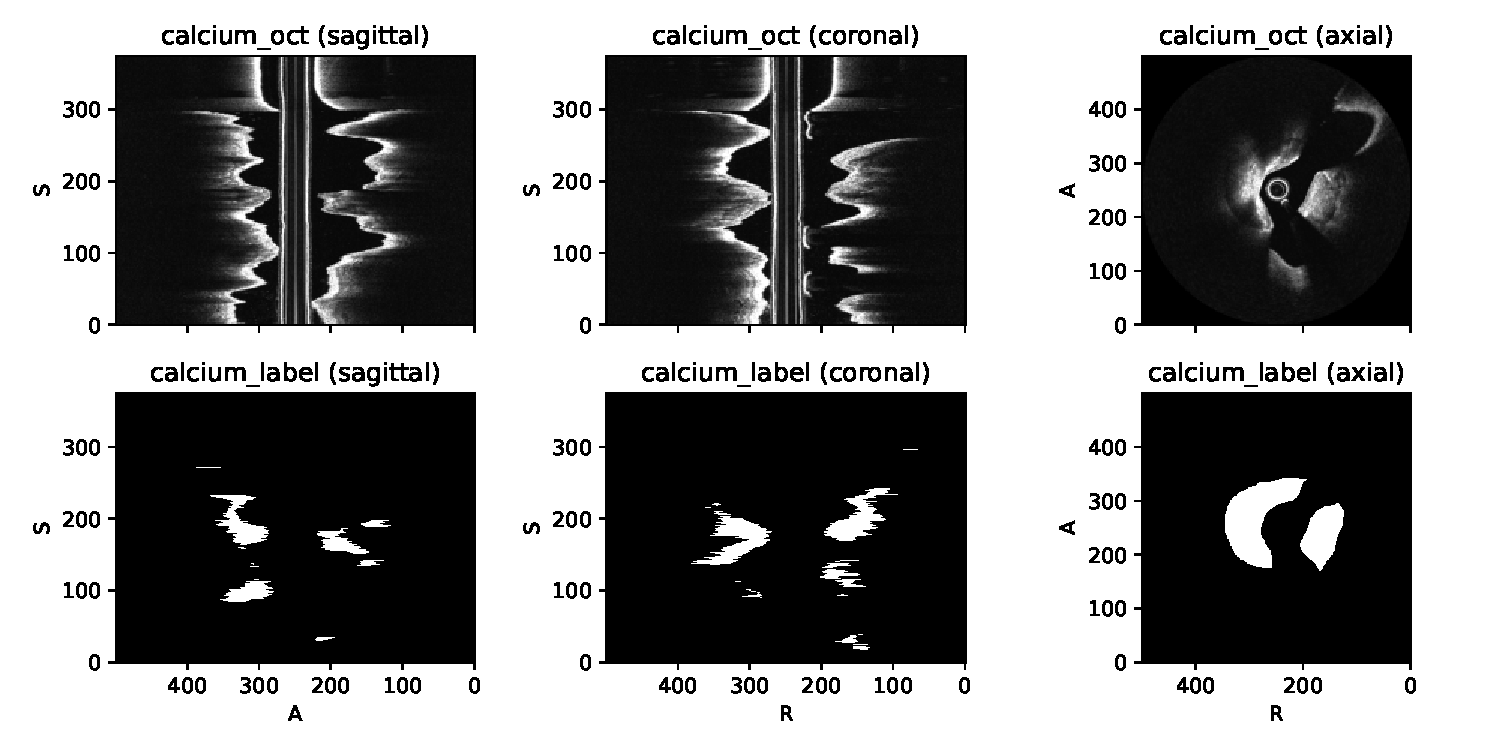
\includegraphics[width=1\linewidth]{figures/fig_datasets_calcium_oct_sample.pdf}
        \caption{An example of an annotated image from the Calcium OCT dataset.}
        \label{fig:calcium-oct}
    \end{subfigure}%
    \hfill
    \begin{subfigure}[t]{0.49\textwidth}
        \centering
        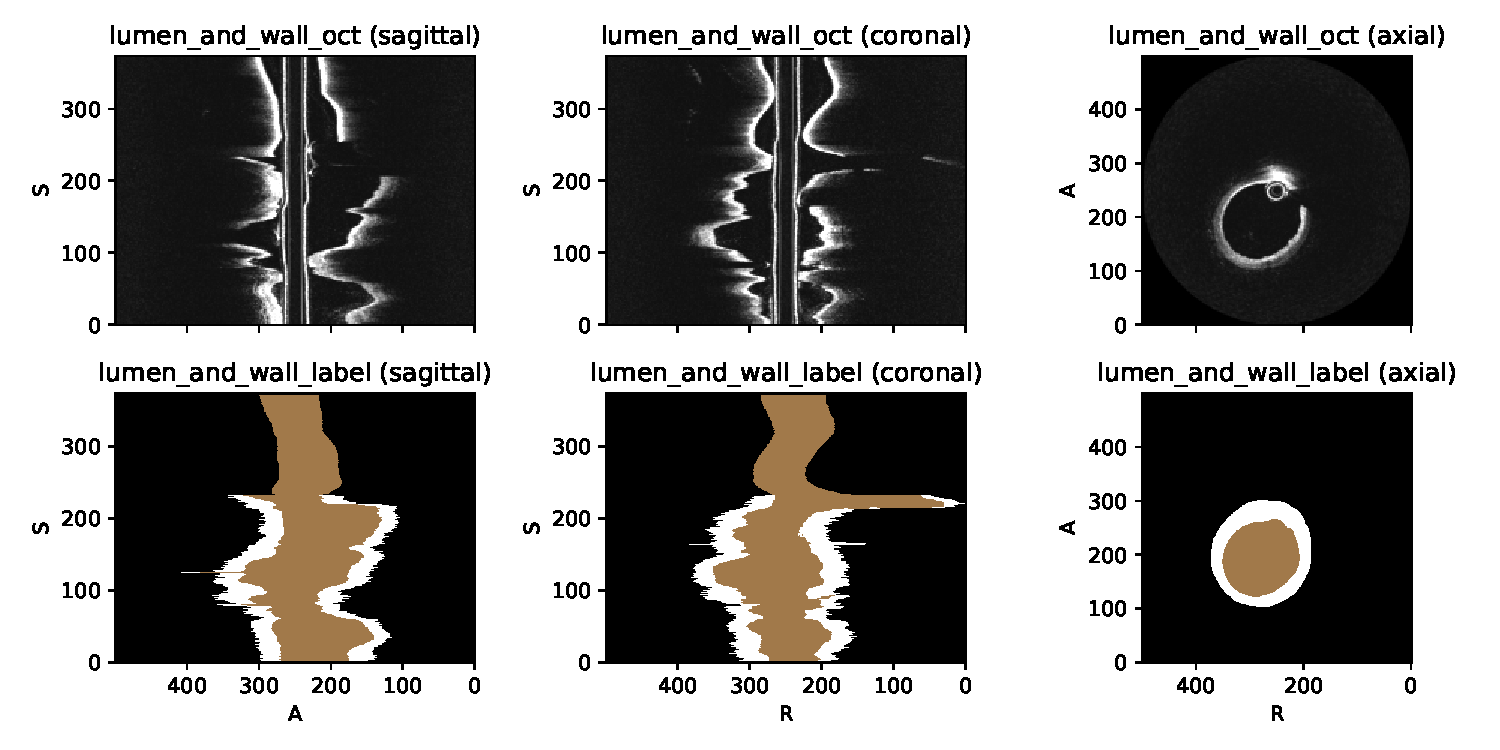
\includegraphics[width=1\linewidth]{figures/fig_datasets_law_oct_sample.pdf}
        \caption{An example of an annotated image from the Lumen and Wall OCT dataset (LaW OCT).}
        \label{fig:lumen-and-wall-oct}
    \end{subfigure}
    \caption{Examples of annotated Calcium OCT (a) and LaW OCT (b) images. Top, the original OCT image from the middle slice across three axes, displayed as three panels from left to right. Bottom, the corresponding segmentation masks.}
    \label{fig:annotated-oct}
\end{figure}

\subsubsection{Data Splitting}

% Each dataset has unique characteristics and is divided into training, validation, and testing sets, except for the unannotated datasets, which are used for self-supervised pre-training.
Calcium OCT has one class: calcium. The size of each image is $500\times 500$, while the depth varies between $375$ and $539$. Examples of Calcium OCT images are shown in Figure~\ref{fig:calcium-oct}. The dataset is split into 6 training volumes and 2 test volumes, and the training volumes are further divided into 3 folds of training and validation sets. In each fold, a model is trained using the training set, and the best model is selected using the validation set then evaluated on the test set not seen during training. Finally, performance data across 3 folds are averaged to report the final performance. This is done to ensure a robust evaluation of the methods.

LaW OCT has 2 classes: lumen and wall. The size of each image is $500\times 500$, while the depth varies between $270$ and $540$. Examples of LaW OCT images are shown in Figure~\ref{fig:lumen-and-wall-oct}. The dataset is split into 16 training volumes and 4 test volumes. 

The unannotated datasets are of size $500\times 500$ and varying depths. They are not split into training and test sets because they are only used for self-supervised pre-training. However, each self-supervised learning algorithm may divide the unannotated datasets into training and validation sets to track convergence. Examples of unannotated OCT images are shown in Figure~\ref{fig:unannotated-oct}.

\begin{figure}[hbt]
    % \centering
    \begin{subfigure}[t]{0.49\textwidth}
        \centering
        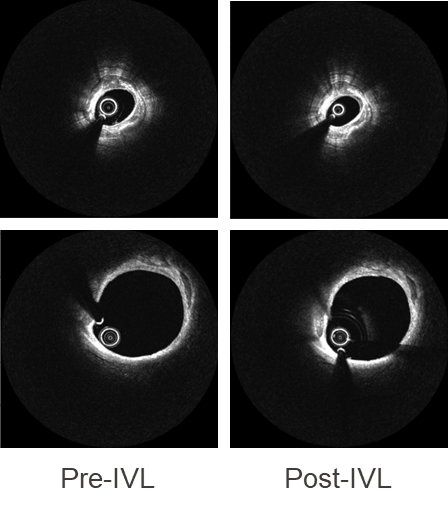
\includegraphics[width=0.65\linewidth]{figures/fig_datasets_coregistered_prepostivl.png}
        \caption{Two examples (top and bottom) of co-registered images between Pre-IVL (left) and Post-IVL (right)}
        \label{fig:co-registered-oct}
    \end{subfigure}%
    \hfill
    \begin{subfigure}[t]{0.49\textwidth}
        \centering
        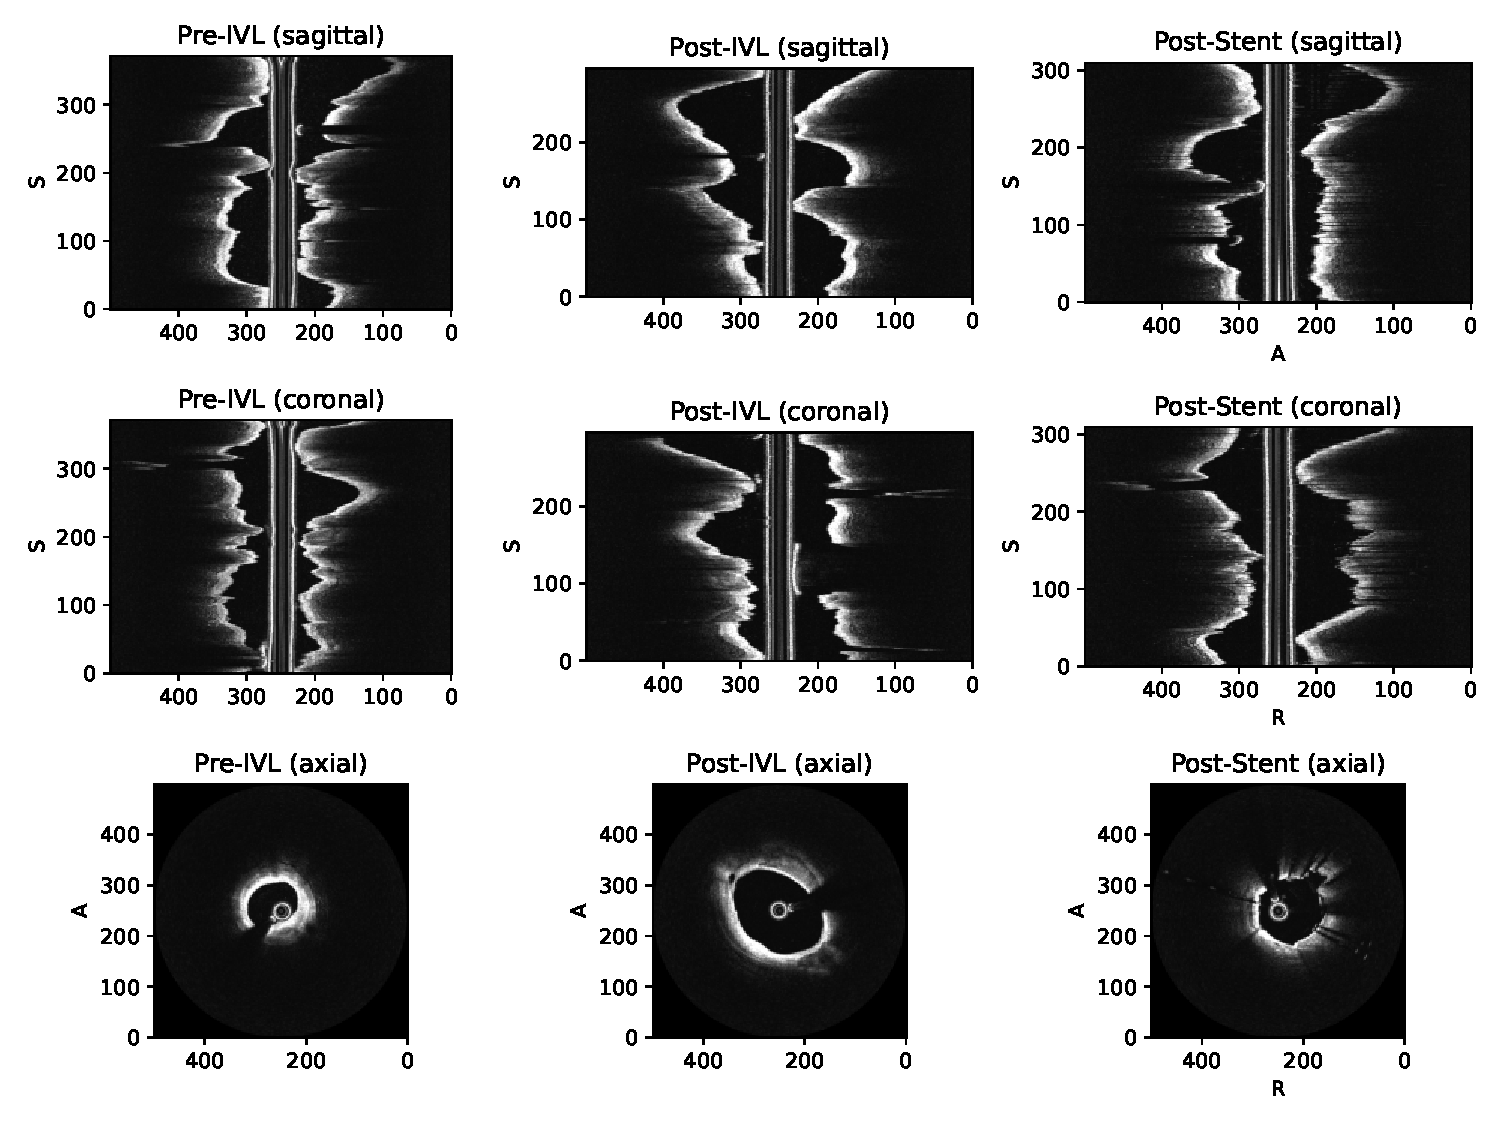
\includegraphics[width=1\linewidth]{figures/fig_datasets_unlabeled_oct_sample.pdf}
        \caption{Examples of unannotated OCT images Pre-IVL (left), Post-IVL (middle), and Post-Stent (right), taken from the middle slice across three axes arranged from top to bottom}
        \label{fig:unannotated-oct}
    \end{subfigure}
    \caption{Examples of unannotated Calcium OCT images.}%For each image, the top row shows the original image at the middle slice across three axes, while the bottom row displays the corresponding segmentation masks.}
\end{figure}

\newpage
\section{Algorithms}
In this section, we describe various learning methods for calcium segmentation, categorizing them into supervised and self-supervised approaches. The key difference lies in whether the approach requires human-annotated data for training. As the names suggest, "supervised" learning requires annotated data, whereas "self-supervised" learning does not.

Supervised learning can be achieved in two manners. The first and more straightforward method is to train a model from scratch using only the Calcium OCT dataset. The second method involves pre-training a model on a different annotated dataset ("supervised pre-training") before fine-tuning it on Calcium OCT for calcium segmentation ("transfer learning" or "fine-tuning"). For example, we could use the LaW OCT dataset to teach a model about the general anatomy of the artery before re-purposing it to identify calcified plaques in the Calcium OCT dataset. 

Self-supervised learning involves pre-training a model on an unannotated dataset followed by fine-tuning it on Calcium OCT for calcium segmentation. There are several methods to pre-train a model using unannotated data. For example, one approach involves artificially masking a small portion of an OCT image and training the model to predict the missing content. As the model gets better at filling in the blank, it simultaneously gains more understanding of the arterial anatomy, which can enhance its ability to identify calcified plaques. This approach highlights the innovative nature of SSL, where the model learns valuable features even in the absence of explicit labels.

%The key difference between supervised and self-supervised in this study lies in whether the pre-training process requires human annotation. It is important to note that CLIP is typically categorized as a weakly supervised learning method since it relies on human annotations to co-register pairs of different modalities. However, as we advance towards automatic co-registration, we have opted to classify it under self-supervised learning for simplicity. >>> moved to CLIP subsection below.

\subsection{Supervised Learning}
\subsubsection{nnUNet}\label{sec:design:nnunet}
nnUNet is a self-configuring framework for medical image segmentation~\cite{Isensee2020}. First, a data fingerprint must be provided to nnUNet, which specifies the number of image modalities, the normalization process for each modality, and the number of segmentation classes. Additional details such as intensity range, image spacing, shape, and resolution are derived from the metadata. Using this fingerprint, nnUNet automatically determines the network topology, sampling strategy, data augmentation approach, batch size, and patch size for the training process. Notably, nnUNet also offers a supervised pre-training pipeline, allowing the model to be trained on other datasets before being fine-tuned on the target dataset.

We designed two approaches to apply the nnUNet algorithm. The first approach involves directly training the model on the Calcium OCT dataset. The second approach involves pre-training the model on the LaW OCT dataset before fine-tuning it for calcium segmentation. 

nnUNet offers both 2D and 3D segmentation architectures, as well as a cascade 3D architecture combining full-resolution and low-resolution networks. Our preliminary experiments indicated that the 2D and 3D architectures outperformed the cascade architecture. Consequently, we decided to use only the 2D and 3D architectures for the remainder of our experiments. The cascade architecture will not be discussed further.

\subsubsection{SegFormer}
SegFormer is a transformer-based model that integrates multi-resolution feature fusion through simple multi-layer perceptrons (MLP~\cite{Rumelhart1986})~\cite{Xie2021SegFormer}. Pre-trained on the ADE20k dataset~\cite{Zhou2018}, SegFormer mirrors U-Net's encoder by downsampling input images via overlap patch merging, which unifies adjacent patches into a single unit. This process allows the model to capture the features at various resolutions. Furthermore, SegFormer utilizes these multi-resolution features with an All-MLP decoder, which aligns lower-resolution features with the channels of their higher-resolution counterparts. The decoder then upsamples the features up to the original resolution and concatenates them with the higher-resolution features, ultimately predicting the segmentation masks using only MLPs and upsampling layers. 

SegFormer architectures comes in various sizes, from MiT-B1 to MiT-B5, with the largest model, MiT-B5, containing 84.7M parameters. We fine-tuned the largest pre-trained model on Calcium OCT for 80,000 iterations, which was sufficient for the model to converge.

\subsubsection{RADIO}
RADIO is a distillation framework that enables the use of multiple vision foundational models as teachers \cite{Ranzinger2024RADIO}. The framework was assessed on 2D segmentation tasks, incorporating batch normalization and linear projection in the decoder head. In alignment with this evaluation protocol, we employed their pre-trained Visual Transformer (ViT) model. Specifically, we utilized the RADIO ViT-H/16 model and fine-tuned it on the Calcium OCT dataset. The training was conducted for 80,000 iterations, which was determined to be adequate for model convergence.

\subsubsection{SuPreM}~\label{sec:design:suprem}
SuPreM is a supervised pre-training method specifically designed for 3D medical image segmentation \cite{Li2024}. It involves training models on a large scale dataset of CT imaging volumes before fine-tuning. Among the models pre-trained with SuPreM, we chose the SwinUNETR model~\cite{Tang2022} due to its reported superior performance and fine-tuned it on the Calcium OCT dataset. It is important to note that the publicly available models have been pre-trained on 2,100 CT volumes, rather than 9,262, as the authors have not yet released the fully pre-trained versions.

SwinUNETR is a transformer-based model designed for segmenting brain tumors in 3D MRI images. Its architecture is built upon the Swin Transformer encoder, extracting hierarchical features from the input image ~\cite{Liu2021Swin}. The model also includes a CNN-based decoder, UNETR, featuring convolutional layers with upsampling and skip connections to merge features across different levels~\cite{Hatamizadeh2022}. The authors of SwinUNETR proposed a self-supervised learning algorithm for the model~\cite{Tang2022}. 

To evaluate the SwinUNETR architecture, we conducted three experiments. First, we fine-tuned the SuPreM pre-trained model on Calcium OCT. Second, we fine-tuned the self-supervised SwinUNETR model on Calcium OCT. Third, we trained the SwinUNETR model from scratch on Calcium OCT, which served as a baseline to assess the effectiveness of the previous two experiments. These experiments aimed to evaluate the benefits of pre-training and self-supervised learning in enhancing SwinUNETR's performance on calcium segmentation tasks.

\subsection{Self-Supervised Learning}
\subsubsection{V-JEPA}
V-JEPA is a self-supervised learning method that learns representations by predicting masked parts of a video. It uses a context encoder to make these predictions and compares the predicted latent vectors with those generated by a target encoder, which views the video without masking~\cite{Bardes2024Vjepa}. The author provides ViT models pre-trained using V-JEPA on the VideoMix2M dataset, which contains 2 million videos. 

We conducted two experiments to evaluate the effectiveness of V-JEPA on OCT images. In the first experiment, we fine-tuned the V-JEPA model on Calcium OCT. In the second experiment, we applied V-JEPA pre-training to Unannotated OCT (Dataset ~\ref{enum:unannotated-dataset}) and fine-tuned the resulting model on Calcium OCT. Since the original paper does not address segmentation tasks, we will discuss the implementation of the decoder head in Section~\ref{sec:implementation:vjepa}.

\subsubsection{Genesis}
Genesis is a self-supervised learning method that learns representations by restoring corrupted images to their original version~\cite{Zhou2021}. In the original paper, Genesis is applied to a U-Net architecture, which contains 15M parameters. We adapted the method to the same 3D nnUNet architecture in Section~\ref{sec:design:nnunet}, which has 30M parameters. Thereafter, we applied Genesis pre-training to unannotated OCT images and fine-tuned the resulting model on Calcium OCT.

\subsubsection{CLIP}
Contrastive Language-Image Pre-training (CLIP) is a contrastive learning method that matches encoded vectors of images with their text captions~\cite{Radford2021CLIP}. In our work, we adapted CLIP to OCT images by using co-registered Pre-IVL and Post-IVL images. We used the same nnUNet architecture as described in Section~\ref{sec:design:nnunet}. CLIP pre-training was applied to 3D nnUNet, which was then fine-tuned on the Calcium OCT dataset. To implement this, we modified the code from a publicly available project~\cite{Shariatnia2021}. While the original paper proposed this pre-training framework for aligning language and images, we tailored the framework for aligning co-registered OCT images instead. Details of this adaptation will be discussed in Section~\ref{sec:implementation:clip}. 

It is important to note that CLIP is typically considered a weakly supervised learning method because it relies on human co-registration of image pairs. However, given the minimal cost of co-registration and as the field is advancing towards automatic co-registration, we have opted to classify CLIP under self-supervised learning for simplicity. 

%%%%%%%%%%%%%%%%%%%%%%%%
\chapter{Implementation}
%%%%%%%%%%%%%%%%%%%%%%%%

% The implementation covers some of the implementation details of your project.
% This is not intended to be a low-level description of every line of code that
% you wrote but covers the implementation aspects of the projects.

% This section is usually 3-5 pages.
\section{Supervised Learning}
\subsubsection{nnUNet}
We applied the official nnUNet~\cite{Isensee2020} code on our datasets, adding an early stopping criterion to the optimizer. In particular, we observed that the 3D segmentation performance of nnUNet was significantly worse than its 2D counterpart. To address this, we experimented with different patch sizes for 3D segmentation, diverging from the default settings. Reducing the depth of the original patch size from $112$ to $32$ improved performance significantly. This could be because smaller depth provided the model with more examples to learn from. In the second experiment, we pre-trained the model on LaW OCT before fine-tuning it on Calcium OCT using the supervised pre-training script provided by nnUNet.

\subsubsection{SegFormer}\label{sec:implementation:segformer}
We adopted the pre-trained SegFormer model along with a training script from MMSegmentation~\cite{mmseg2020}. Since SegFormer is designed exclusively for 2D segmentation, we pre-processed our Calcium OCT dataset into 2D images before training the model on the reformatted data. To ensure a fair comparison, we also maintained the same three folds and testing set as those used in nnUNet.

\subsubsection{RADIO}
We utilized the pre-trained RADIO's ViT model and its training script available in MMSegmentation~\cite{mmseg2020}. Since RADIO, like SegFormer, only supports 2D segmentation, we used the same pre-processed datasets as described in Section~\ref{sec:implementation:segformer}.

\subsubsection{SuPreM}
SuPreM provides official pre-trained models and code~\cite{Li2024}. Accordingly, we reformatted our Calcium OCT dataset to align with the format of SuPreM's datasets, while ensuring that the three folds and testing set remained consistent with those used in other experiments within this study. We three experiments, as outlined in Section~\ref{sec:design:suprem}, employing the official script from SuPreM.

\section{Self-Supervised Learning}
\subsubsection{V-JEPA}\label{sec:implementation:vjepa}
We developed three segmentation decoder heads for the Vision Transformer (ViT) pre-trained with V-JEPA, because it had previously been evaluated solely on classification tasks using an encoder-only transformer referred to as attentive decoder. To extend its utility to segmentation tasks, we designed an attentive decoder head for segmentation, drawing inspiration from the MAE decoder~\cite{He2022}, which directly predicts pixel values. Specifically, our decoder head employs an encoder-only transformer of 1 depth and 12 attention heads, followed by a linear projection layer that transforms embedding vectors into a vector of size \(\{\text{patch size} \times \text{patch size} \times \text{number of classes}\}\). 

In addition, we experimented with alternative decoding architectures, such as a simple batch normalization layer followed by a linear projection, similar to the adaptations made in RADIO~\cite{Ranzinger2024RADIO} and DINOv2~\cite{Oquab2024dinov} for segmentation tasks. Both variations are illustrated in Figure~\ref{fig:vjepa-attentive-and-batchnorm-decoder-head}. 

\begin{figure}[ht]
    \centering
    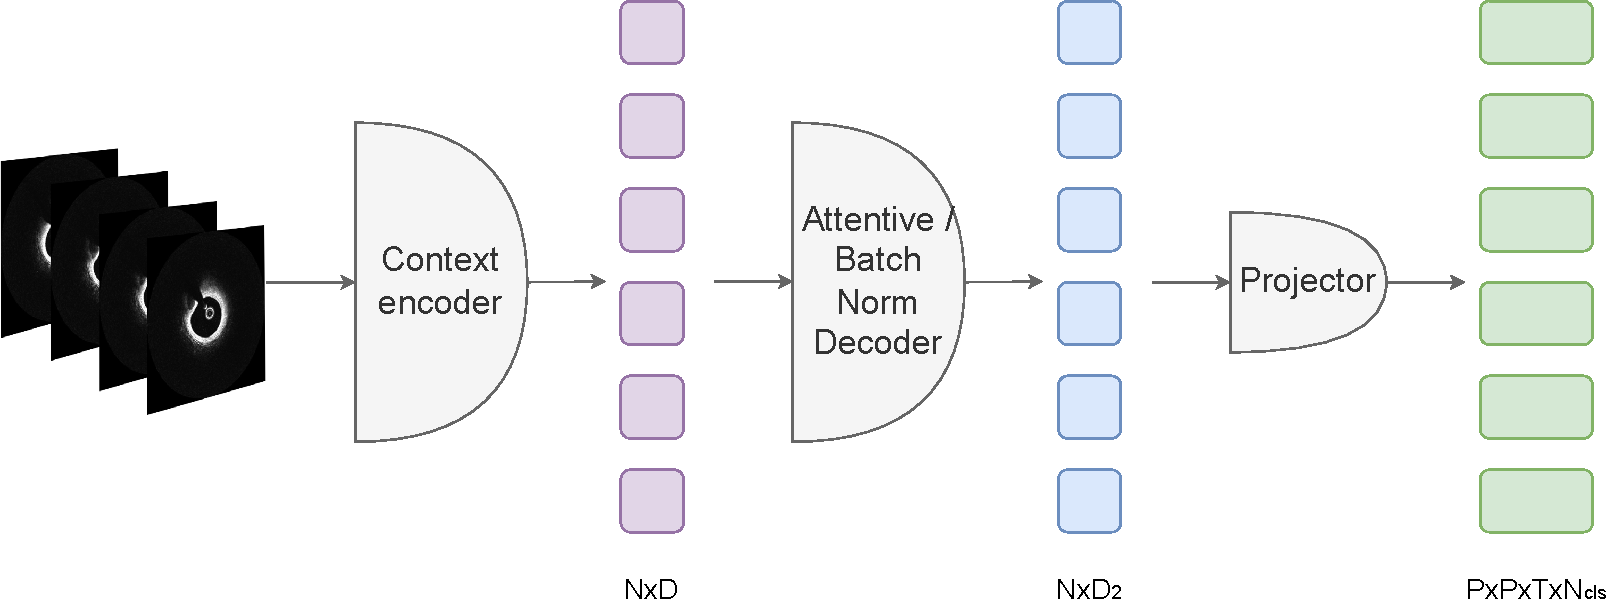
\includegraphics[width=0.6\linewidth]{figures/fig_implementation_vjepa_attentive_and_batchnorm_decoder.pdf}
    \caption{Attentive and linear batch normalization decoder head for ViT (V-JEPA).}
    \label{fig:vjepa-attentive-and-batchnorm-decoder-head}
\end{figure}%

Further, inspired by SegFormer~\cite{Xie2021SegFormer}, we developed multi-feature decoder with a multi-layer perceptron (MLP) on each feature vector at different depths, followed by a linear projection to combine those features into a segmentation mask. This approach allows the decoder to leverage multiple features at various levels. However, unlike SegFormer, our method does not downsample each feature, thereby not explicitly forcing them to lower resolutions. Ultimately, this method allowed us to utilize ViT pre-trained with V-JEPA, ViT (V-JEPA), in our segmentation task. The multi-feature decoder head is shown in Figure~\ref{fig:vjepa-multi-feature-decoder-head}.

\begin{figure}[ht]
    \centering
    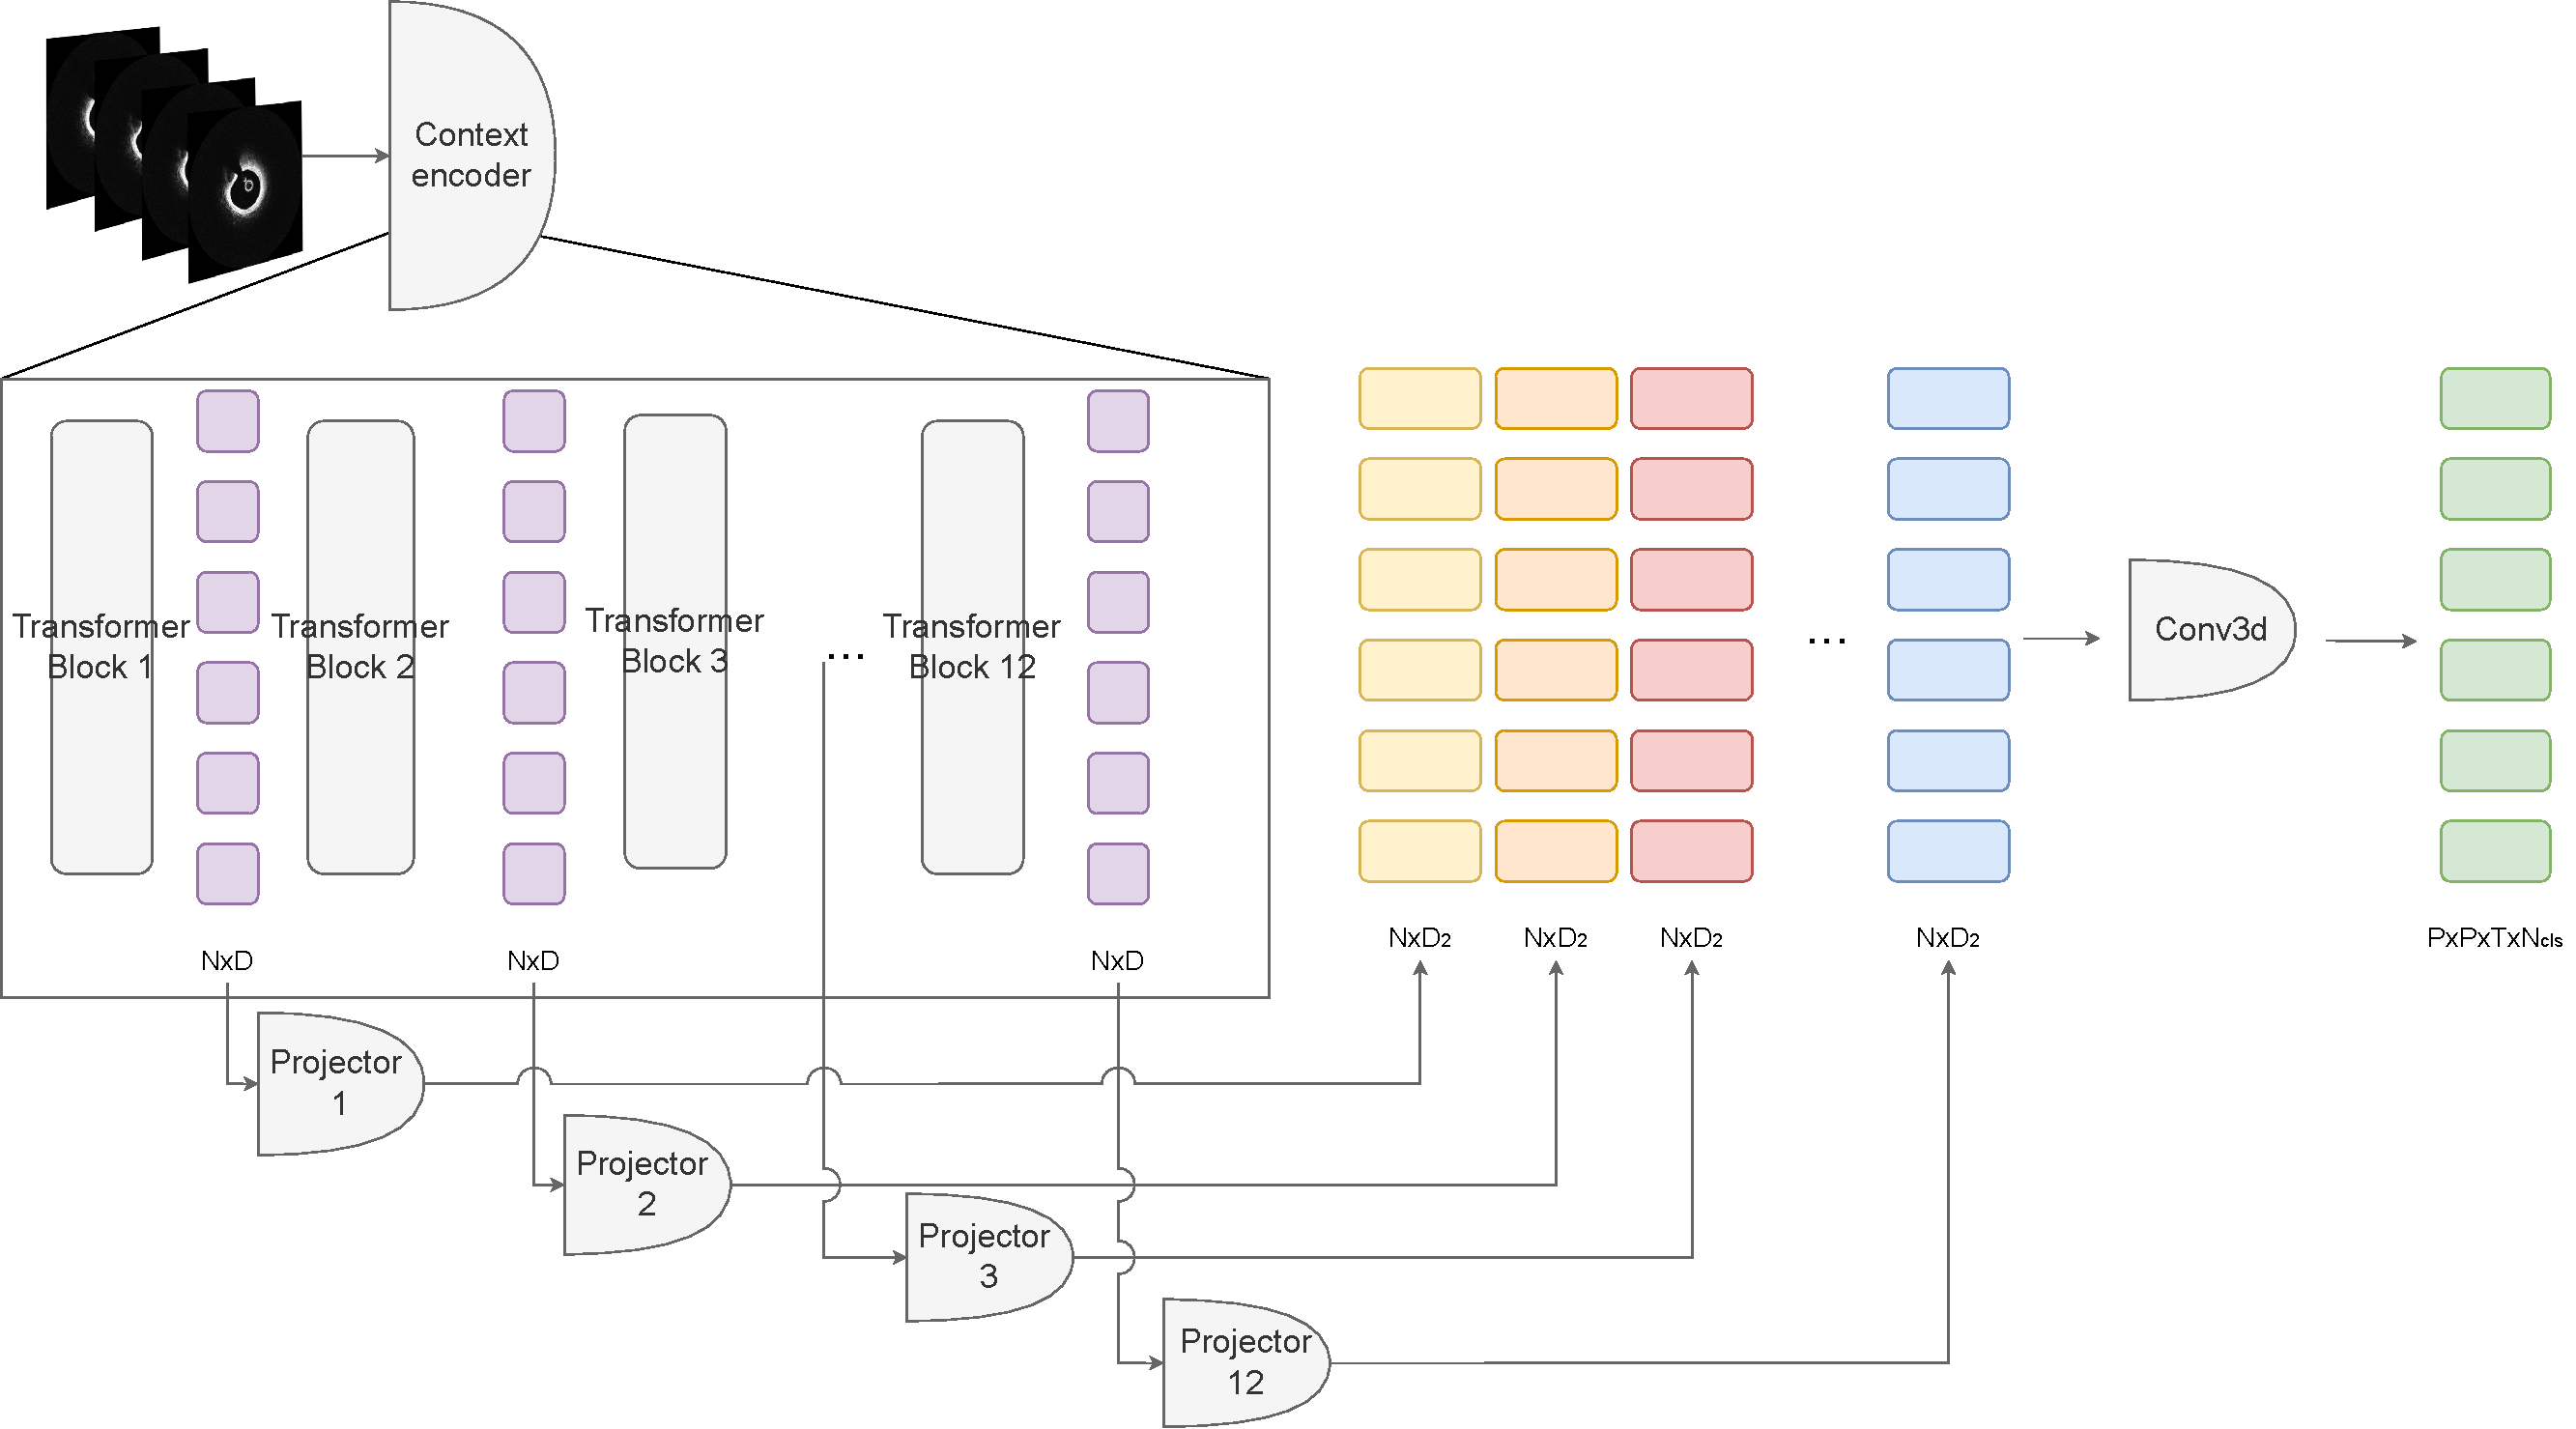
\includegraphics[width=1.0\linewidth]{figures/fig_implementation_vjepa_multifeat.pdf}
    \caption{A multi-feature decoder head. Feature at each transformer block is projected to the same dimension and concatenated before being passed to a convolutional layer that produces the segmentation mask.}
    \label{fig:vjepa-multi-feature-decoder-head}
\end{figure}

\subsubsection{Genesis}
We altered the official code for Genesis provided by the authors~\cite{Zhou2021} by adding a pre-processing step to the method. Genesis implementation begins with an initial pre-processing step on unannotated OCT images, where small cubes of size $64\times 64\times 64\times 32$ are sampled from the volumes. These cubes are then dynamically corrupted during the Genesis pre-training process. The authors recommend sampling $96$ cubes per volume, noting that increasing this number does not necessarily improve the performance and adds computation cost. Following this recommendation, we implemented an additional sampling strategy to enhance the quality of the cubes.

Our strategy involved randomly sampling $96$ cubes from each volume, ensuring that the selected cubes contained enough information, given that OCT images often contain substantial background, unlike CT images used in the original paper. We achieved this by applying a thresholding technique, selecting only those cubes with average intensities above a certain threshold. As illustrated in Figure~\ref{fig:genesis-cubes-with-threshold}, the resulting cubes contain meaningful structures such as the artery's lumen and wall. In contrast, without our thresholding strategy, the sampled cubes are dominated by background noise, as shown in Figure~\ref{fig:genesis-cubes-without-threshold}. We trained the model on these cubes until convergence.

\begin{figure}[t]
    \centering
    \begin{subfigure}[t]{0.48\textwidth}
        \centering
        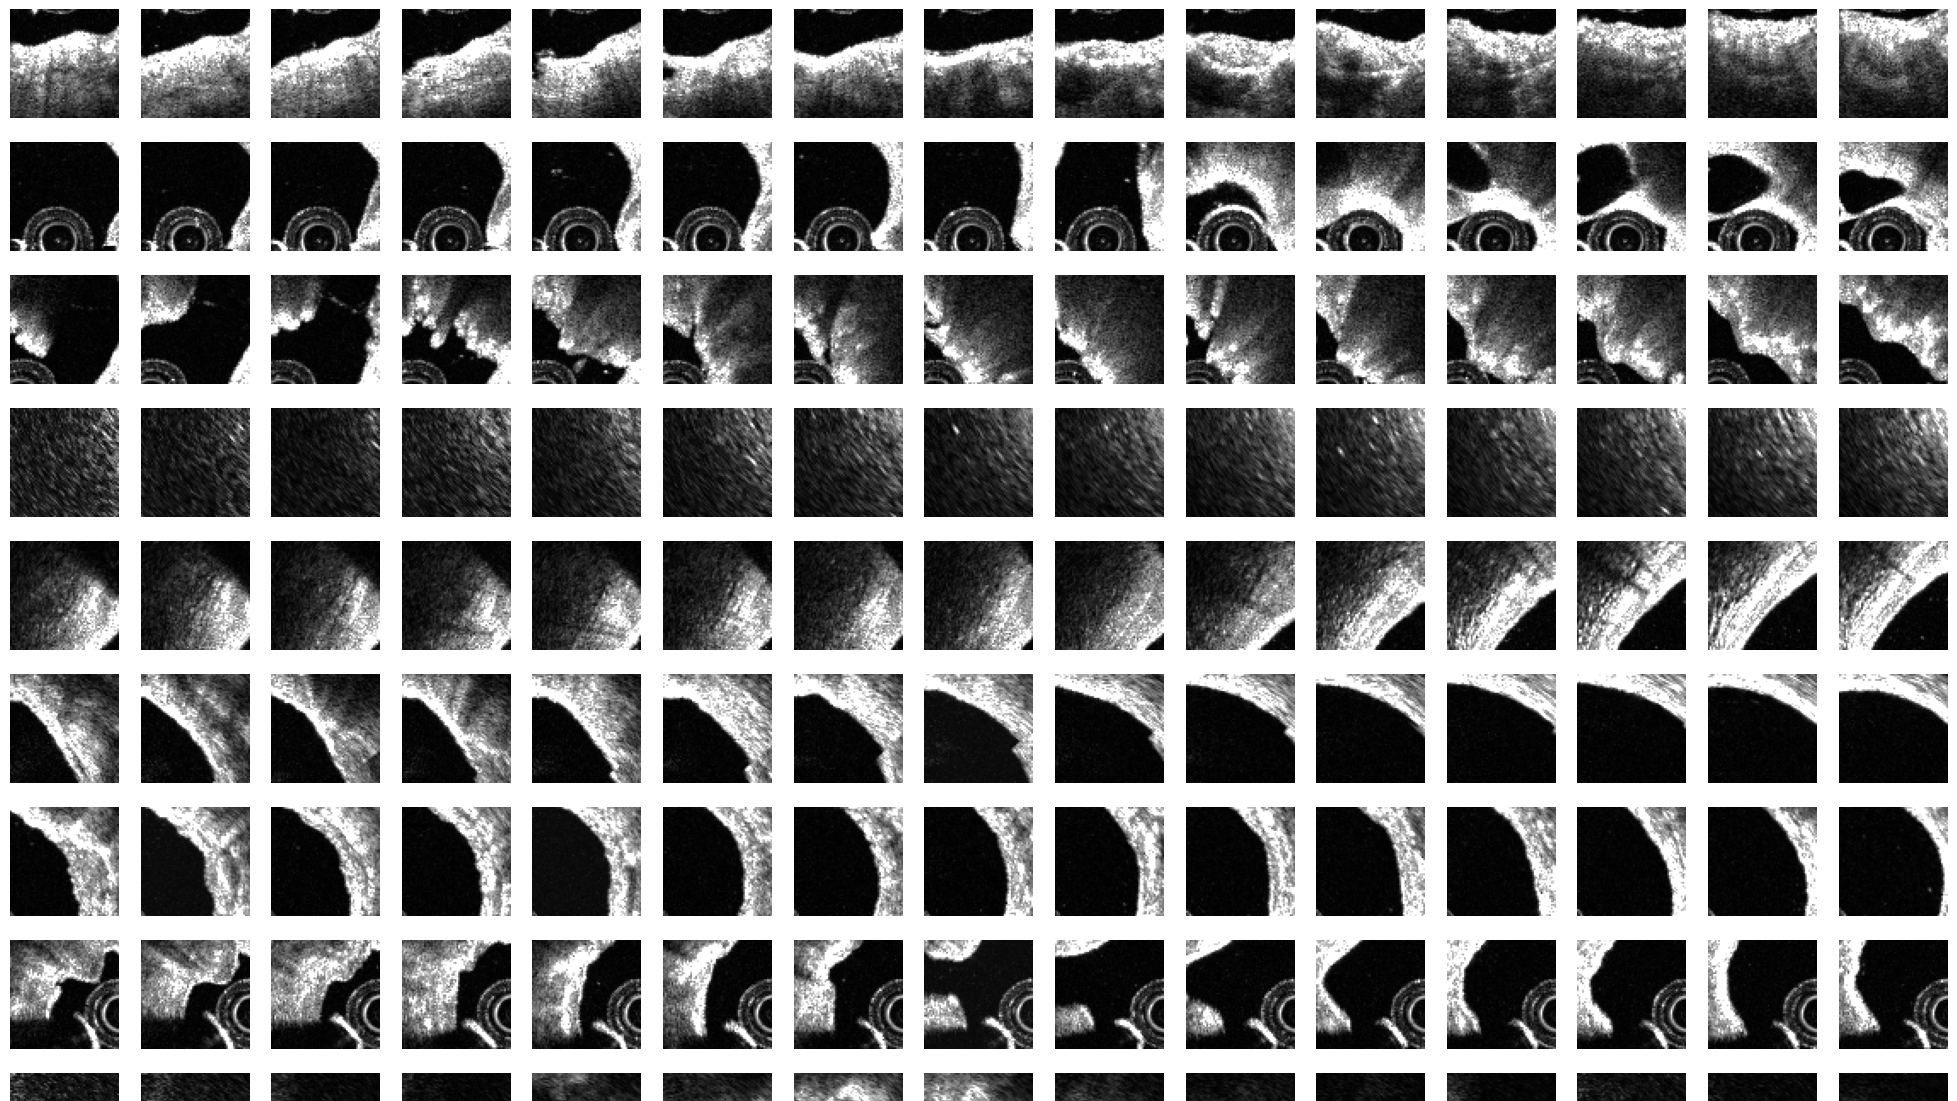
\includegraphics[width=0.9\linewidth]{figures/fig_implementation_genesis_extracted_cube.png}
        \caption{Cubes from unannotated OCT images sampled with the thresholding strategy.}
        \label{fig:genesis-cubes-with-threshold}

    \end{subfigure}%
    \hfill
    \begin{subfigure}[t]{0.48\textwidth}
        \centering
        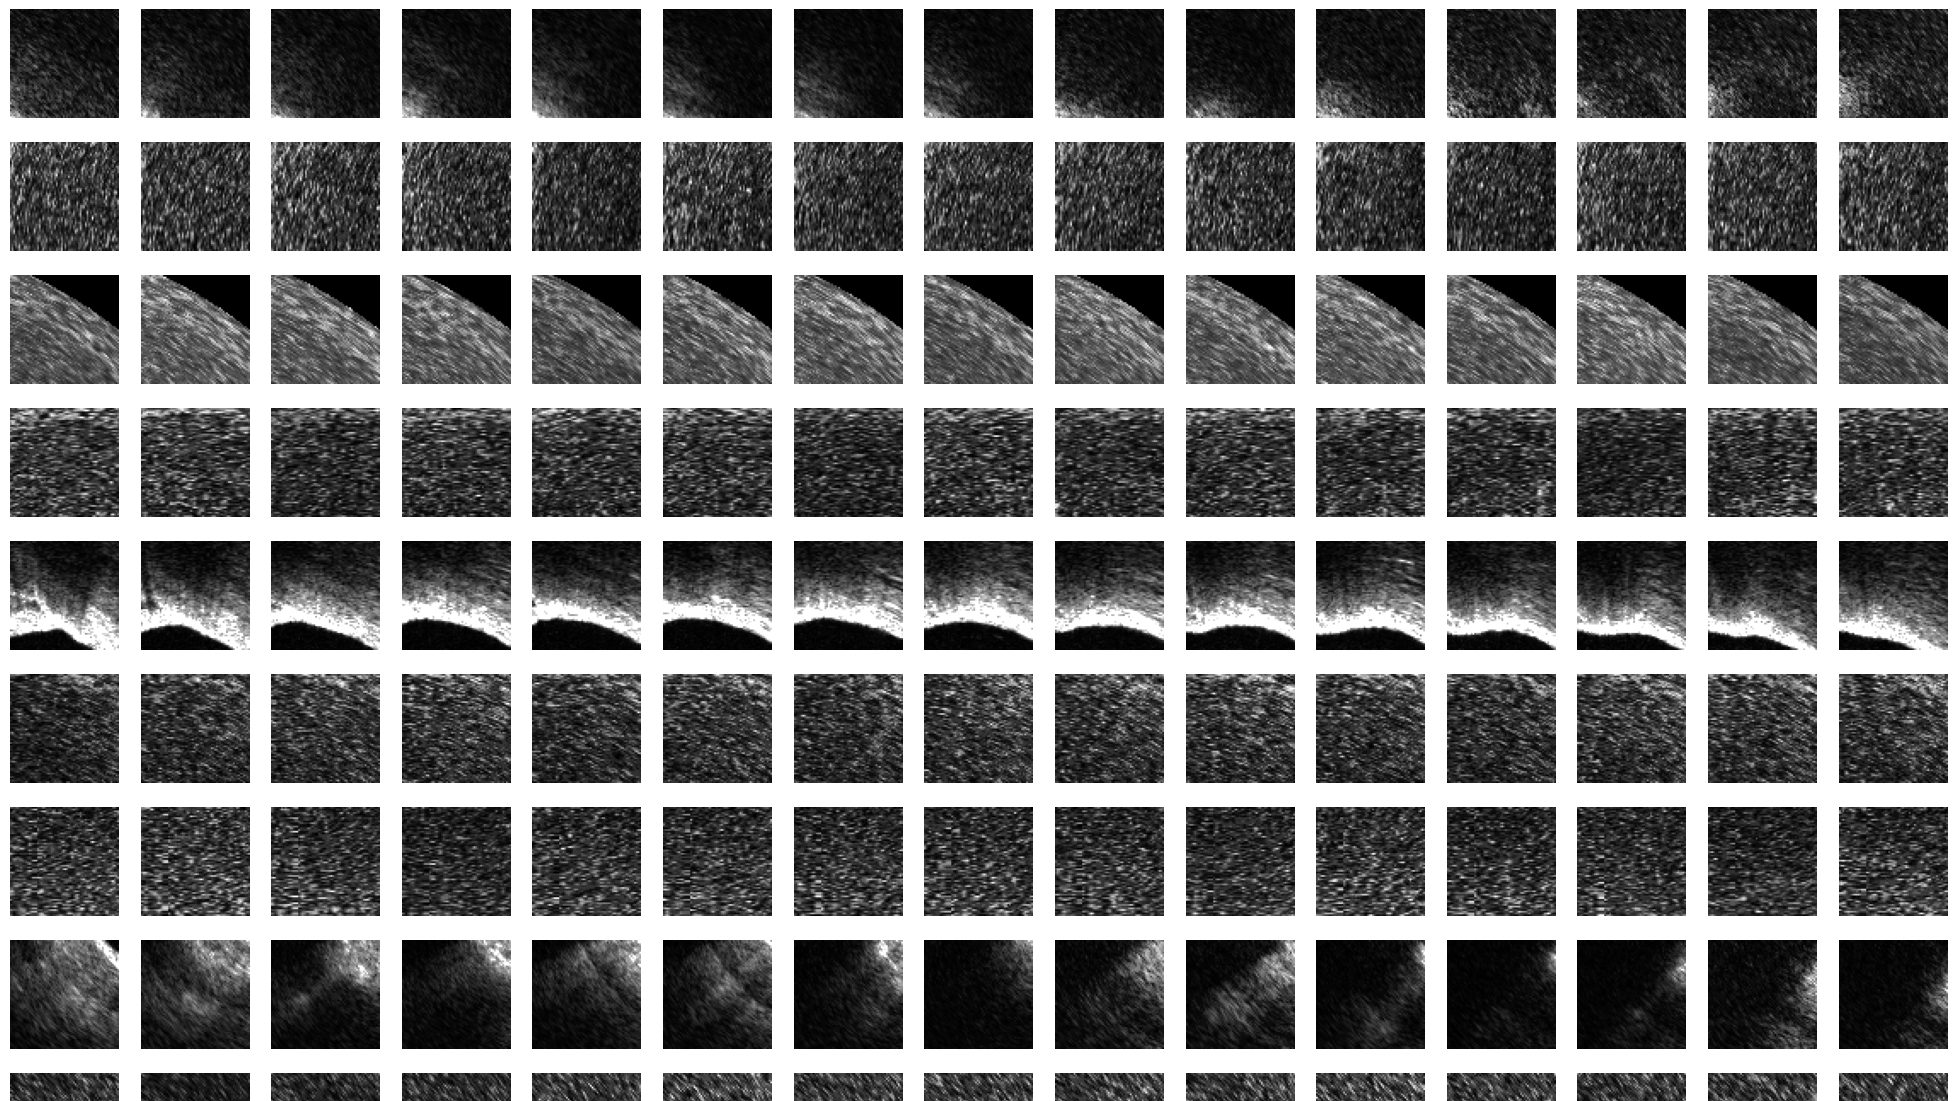
\includegraphics[width=0.9\linewidth]{figures/fig_implementation_genesis_extracted_cube_no_threshold.png}
        \caption{Examples of cubes sampled from unannotated OCT images. Each row represents a sampled cube with slices unrolled along the depth dimension.}
        \label{fig:genesis-cubes-without-threshold}
    \end{subfigure}
    \caption{Samples of cubes from unannotated OCT images. Each row is a sampled cube with slices unrolled along the depth dimension.}
\end{figure}

For fine-tuning, we loaded the pre-trained weights of the model's encoder and decoder into the 3D nnUNet, leaving the segmentation head to be randomly initialized. We then fine-tuned the pre-trained model on the Calcium OCT dataset, utilizing the optimal patch size of $160\times 128\times 32$ (height by width by depth) identified in Section~\ref{sec:result:nnunet}. The nnUNet's training script was used with the same configurations as the supervised pre-training, providing the pre-trained model as the initial weights.

\subsubsection{CLIP}\label{sec:implementation:clip}
We adopted the CLIP model, originally designed for language-image pairs, to work with paired Pre-IVL and Post-IVL volumes by replacing the text encoder with an image encoder. However, this straightforward modification did not result in successful pre-training convergence, necessitating further adjustments using a shared encoder.

Our experiments revealed that using separate encoders and projectors for each modality was less effective than employing a shared encoder and projector. To validate this, we conducted a sanity check by evaluating different encoder and projector configurations. Specifically, we passed the same images through these configurations to see if they could learn to represent the same image as the same vector. We tested three setups: (1) separate encoders and projectors, (2) separate encoders with shared projectors, and (3) shared encoders and projectors. The results showed that the configurations with shared components—either shared projectors or shared encoders and projectors—could match the same image.

Building on these findings, we applied the two successful configurations to the main task of matching co-registered images. Only the configuration with shared encoders and projectors achieved convergence, which is logical as this setup forces the image encoder and projector to learn a representation applicable to both modalities. This process is illustrated in Figure~\ref{fig:clip-oct}. Further details of the experiment are provided in Section~\ref{sec:results:discussion:clip}.

\begin{figure}[hb]
    \centering
    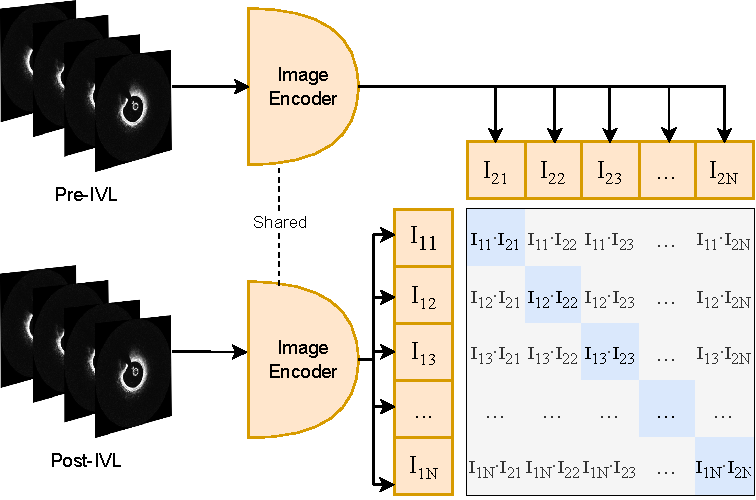
\includegraphics[width=0.65\linewidth]{figures/fig_implementation_clip_oct.pdf}
    \caption{A modified CLIP model for co-registered multi-modal OCT images. Note that the projector is omitted for simplicity. The image encoder and projector are shared across all modalities.}
    \label{fig:clip-oct}
\end{figure}

%%%%%%%%%%%%%%%%%%%%
\chapter{Results and Discussion}
%%%%%%%%%%%%%%%%%%%%

% In the evaluation you convince the reader that your design works as intended.
% Describe the evaluation setup, the designed experiments, and how the
% experiments showcase the individual points you want to prove.

% This section is usually 5-10 pages.
We evaluated the effectiveness of supervised and self-supervised learning algorithms for calcium segmentation of coronary OCT images. All the models were fine-tuned on the training set of Calcium OCT, and the best models were selected using the validation set, which was repeated across 3 folds. These best models were then evaluated against the test set to determine whether they can accurately identify calcified plaques. Performance was measured using the Dice score, a common metric for segmentation tasks, which is defined as follows:

\begin{equation}
    \text{Dice} = \frac{2 \times \text{TP}}{2 \times \text{TP} + \text{FP} + \text{FN}}
\end{equation}

where TP, FP, and FN are true positive, false positive, and false negative, respectively. True positives refer to algorithm-predicted calcium that is present in the ground truth; false positives refer to algorithm-predicted calcium that is absent in the ground truth; and false negatives refer to a lack of algorithm-predicted calcium that is present in the ground truth. The Dice score ranges from 0 to 1, where 1 indicates perfect segmentation. The Dice score was calculated for each patient in the testing set for each fold, and the average Dice score of all folds was reported as the final performance of the model.

\section{Supervised Learning}
\subsection{nnUNet}\label{sec:result:nnunet}
\subsubsection{Effect of Patch Size}
The default configuration of 3D nnUNet has significantly worse performance than 2D nnUNet (0.661 versus 0.753), suggesting that 2D may be generally advantageous over 3D for this task. 

For 3D nnUNet, reducing the depth of the patch size from $112$ to $32$ improves performance significantly, increasing the Dice score from 0.661 to 0.732. The smaller depth potentially allows sectioning of the 3D images into more slices, generating more examples for the model to learn from. By contrast, expanding the width and height of the patch size from $160\times 128$ to $512\times 512$ does not improve performance, decreasing the Dice score from 0.732 to 0.697. This may be due to the localized nature of calcium plaques in OCT images, where a planar expansion along the width and height dimensions is unlikely to provide the model with additional information while reducing examples available for the training process. Alternatively, the expanded images are of larger size and may require a deeper network to handle. The performance of nnUNet on the Calcium OCT dataset is summarized in Figure~\ref{fig:nnunet-results}.

\begin{figure}[h]
    \centering
    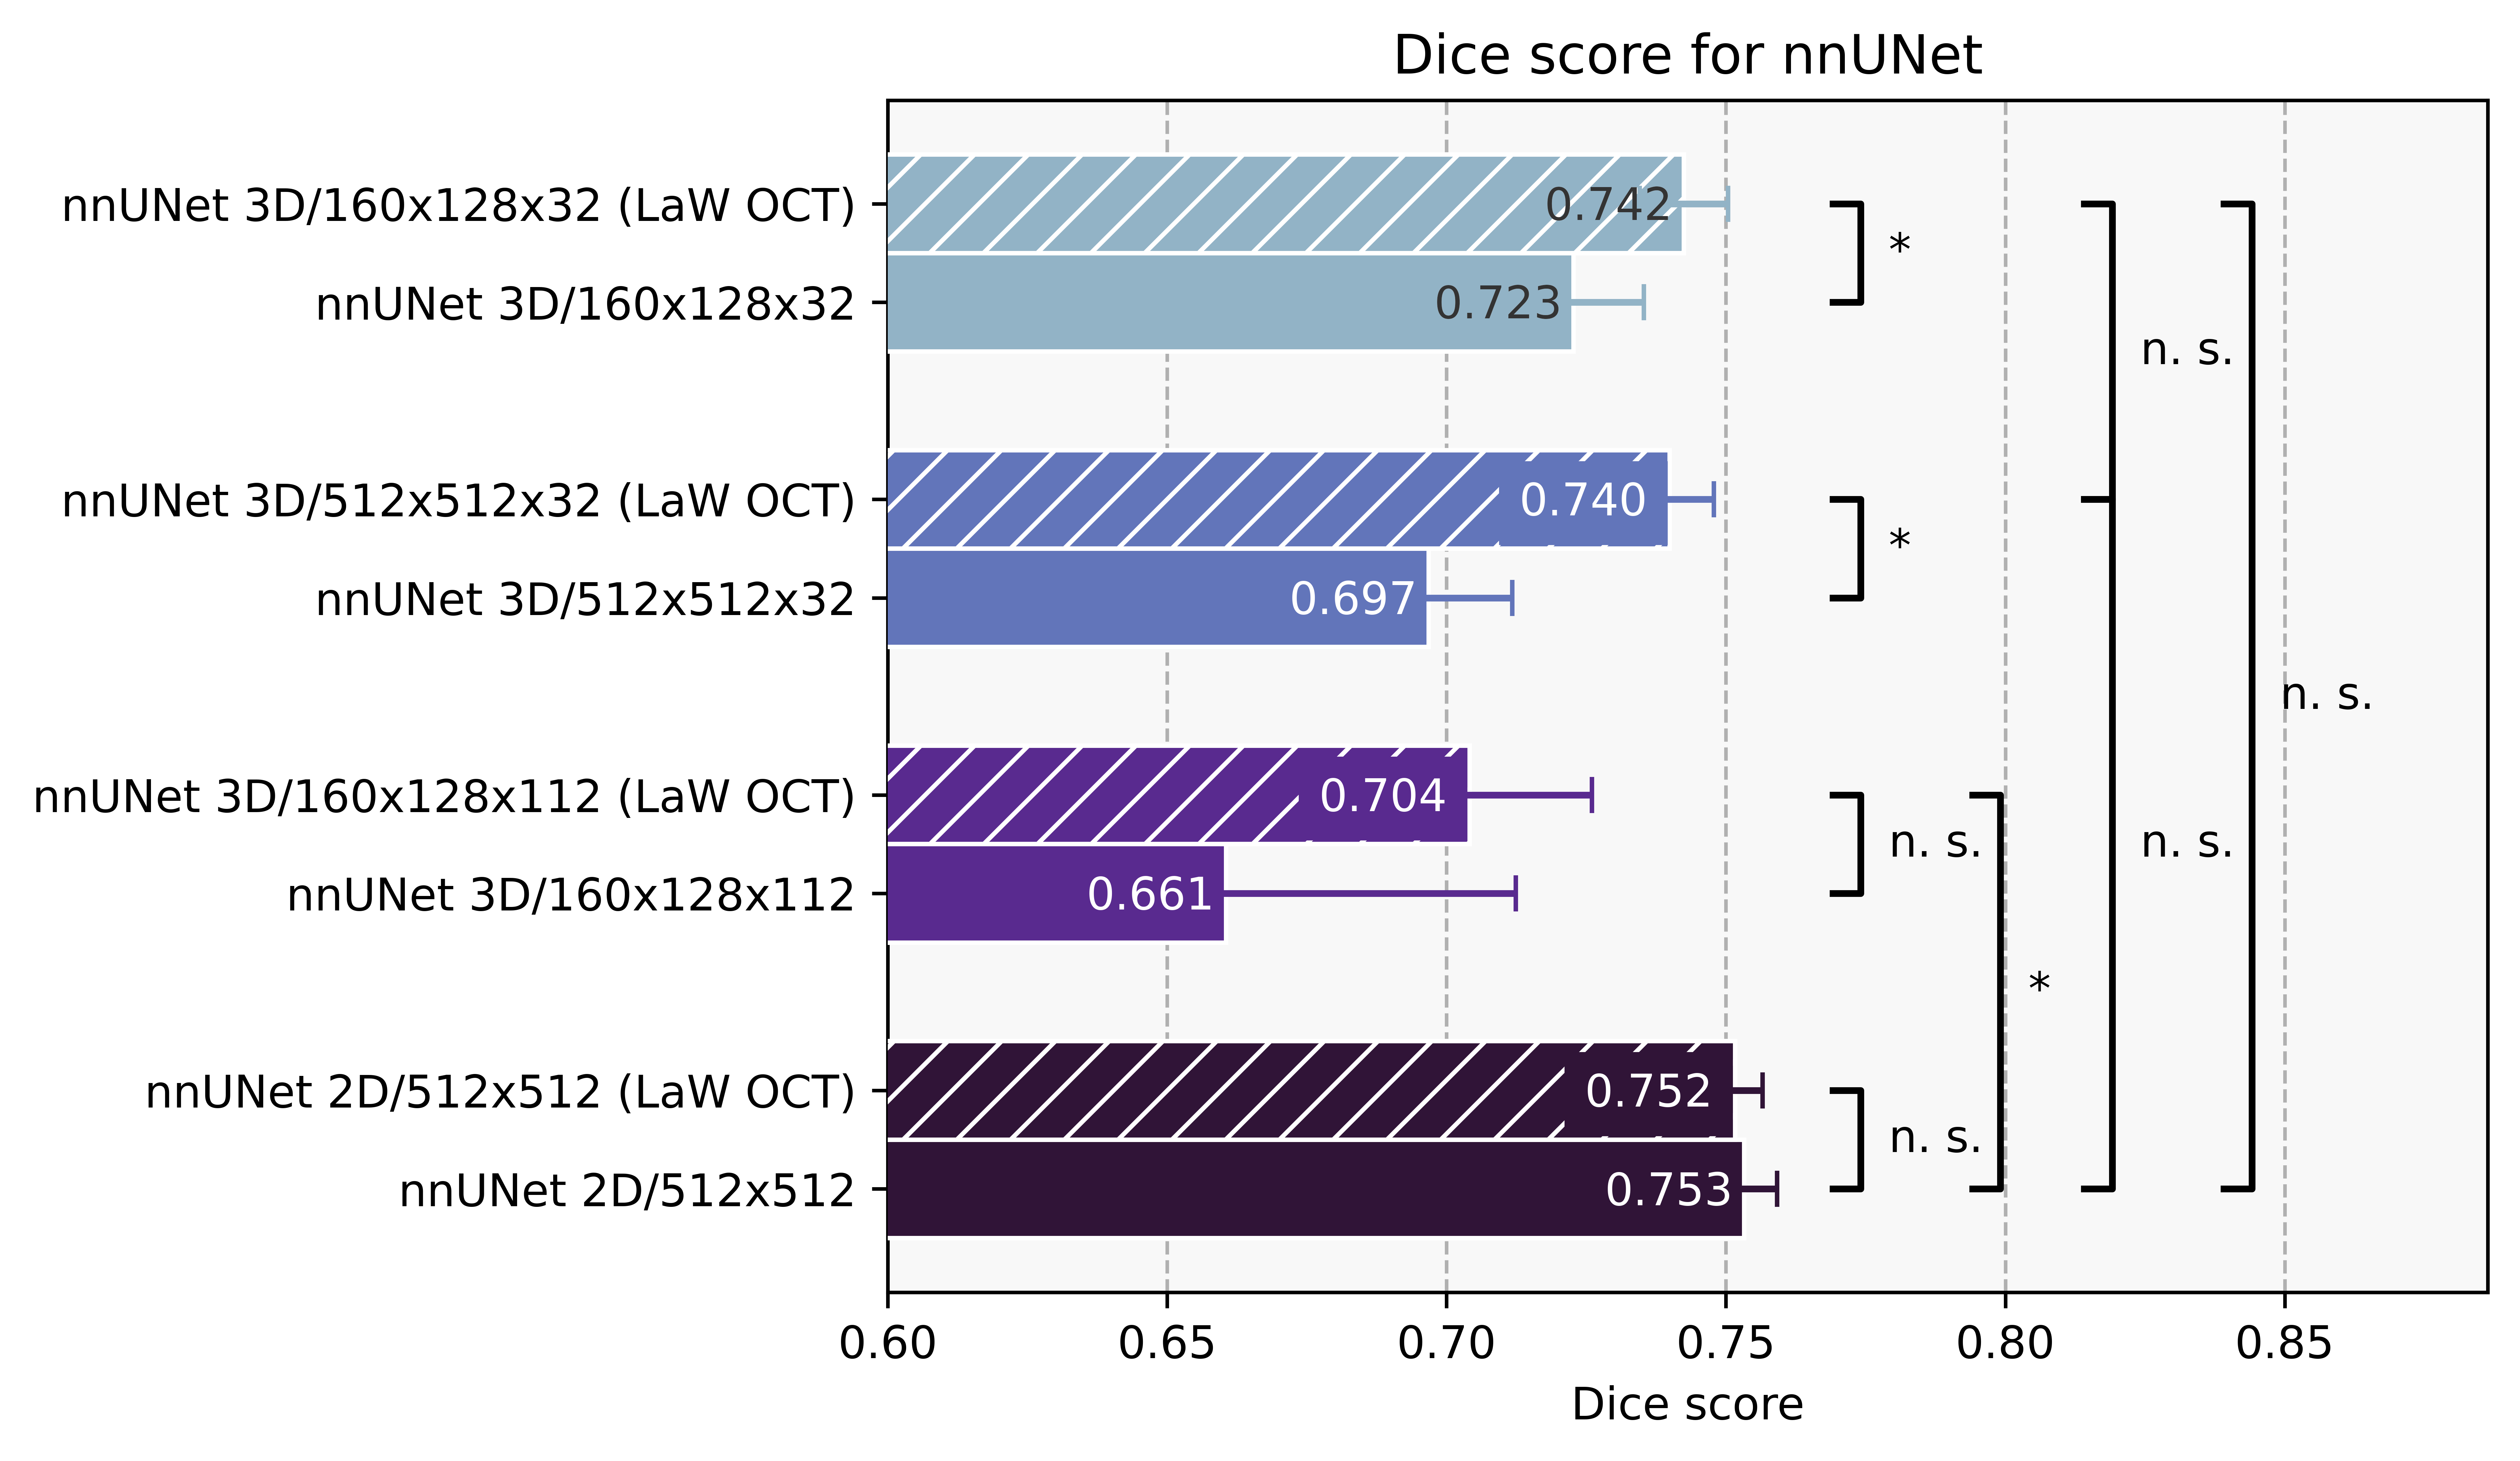
\includegraphics[width=0.8\linewidth]{figures/result_nnunet_results.png}
    \caption{Dice score of variations of nnUNet. Results are grouped according to the patch size used in training. Results in hashes indicate supervised pre-training on the lumen and wall dataset (LaW OCT). 
    }
    \label{fig:nnunet-results}
\end{figure}

\subsubsection{Effect of Pre-training}
Pre-training nnUNet with the lumen and wall dataset (LaW OCT) before fine-tuning it on Calcium OCT confers little benefit to 2D nnUNet (0.752 versus 0.753) but significantly improves 3D nnUNet performance (0.742 versus 0.732 for $160\times 128\times 32$, and 0.740 versus 0.697 for $512\times 512\times 32$). We speculate that, because calcified plaques are typically located around the periphery of artery walls, pre-training with LaW OCT allows the model to learn the features of the walls, which may be helpful for calcium segmentation. These pre-trained 3D nnUNet models (0.742 and 0.740) yielded statistically comparable performance to 2D nnUNet (0.753; Figure~\ref{fig:nnunet-results}). 

\subsubsection{Continuity}
As 2D nnUNet has a better Dice score than 3D nnUNet, it is worth asking whether 3D segmentation provides any advantages at all, or are we better off developing only 2D segmentation models going forward?

We find that 3D models may still be of use, particularly in cases where continuity is necessary. Continuity refers to the consistency of segmentation results across adjacent image slices. Consider three consecutive, closely spaced slices of the same artery. If a calcified plaque is identified in the two outer slices, then it should also be present in the middle slice by continuity. In our research group, we place great emphasis on the continuity of segmentation because one of the use cases is to reconstruct a 3D digital twin of the artery, which can be used for various medical simulations. 

We analyzed correctness (Dice score) versus consistency (continuity) for 2D and 3D nnUNet algorithms as follows (Figure~\ref{fig:nnunet-continuity-vs-correctness}). We performed the continuity analysis on the validation sets of all folds instead of the test set, to increase the number of samples. We defined continuity to be the inverse of changes between adjacent segmentation slices. The mathematical definition is as follows.

\begin{equation}
\text{Continuity} = \left(\frac{1}{M\times (N - 1)}\sum_{i = 1}^{M}\sum_{j = 1}^{N-1} \left| I_{j}^{i} - I_{j+1}^{i}\right|\right)^{-1}
\end{equation}

where $M$ is the number of validation images and $N$ is the number of slices per volume. $I_{j}^{i}$ denotes a segmentation mask of the $j$th slice of the $i$th volume. Using this definition, we tracked the Dice scores of the validation images while progressively applying morphological operations -- first opening and then closing -- to enhance segmentation continuity. We applied different kernel shapes and sizes to smoothen the mask and increase thereby increasing the continuity. The kernels included 3D spheres and ellipsoids. In ellipsoids, the semi-axis in the depth dimension is greater than the others, as discontinuity is likely to occur. 

\begin{figure}[htb]
    \centering
    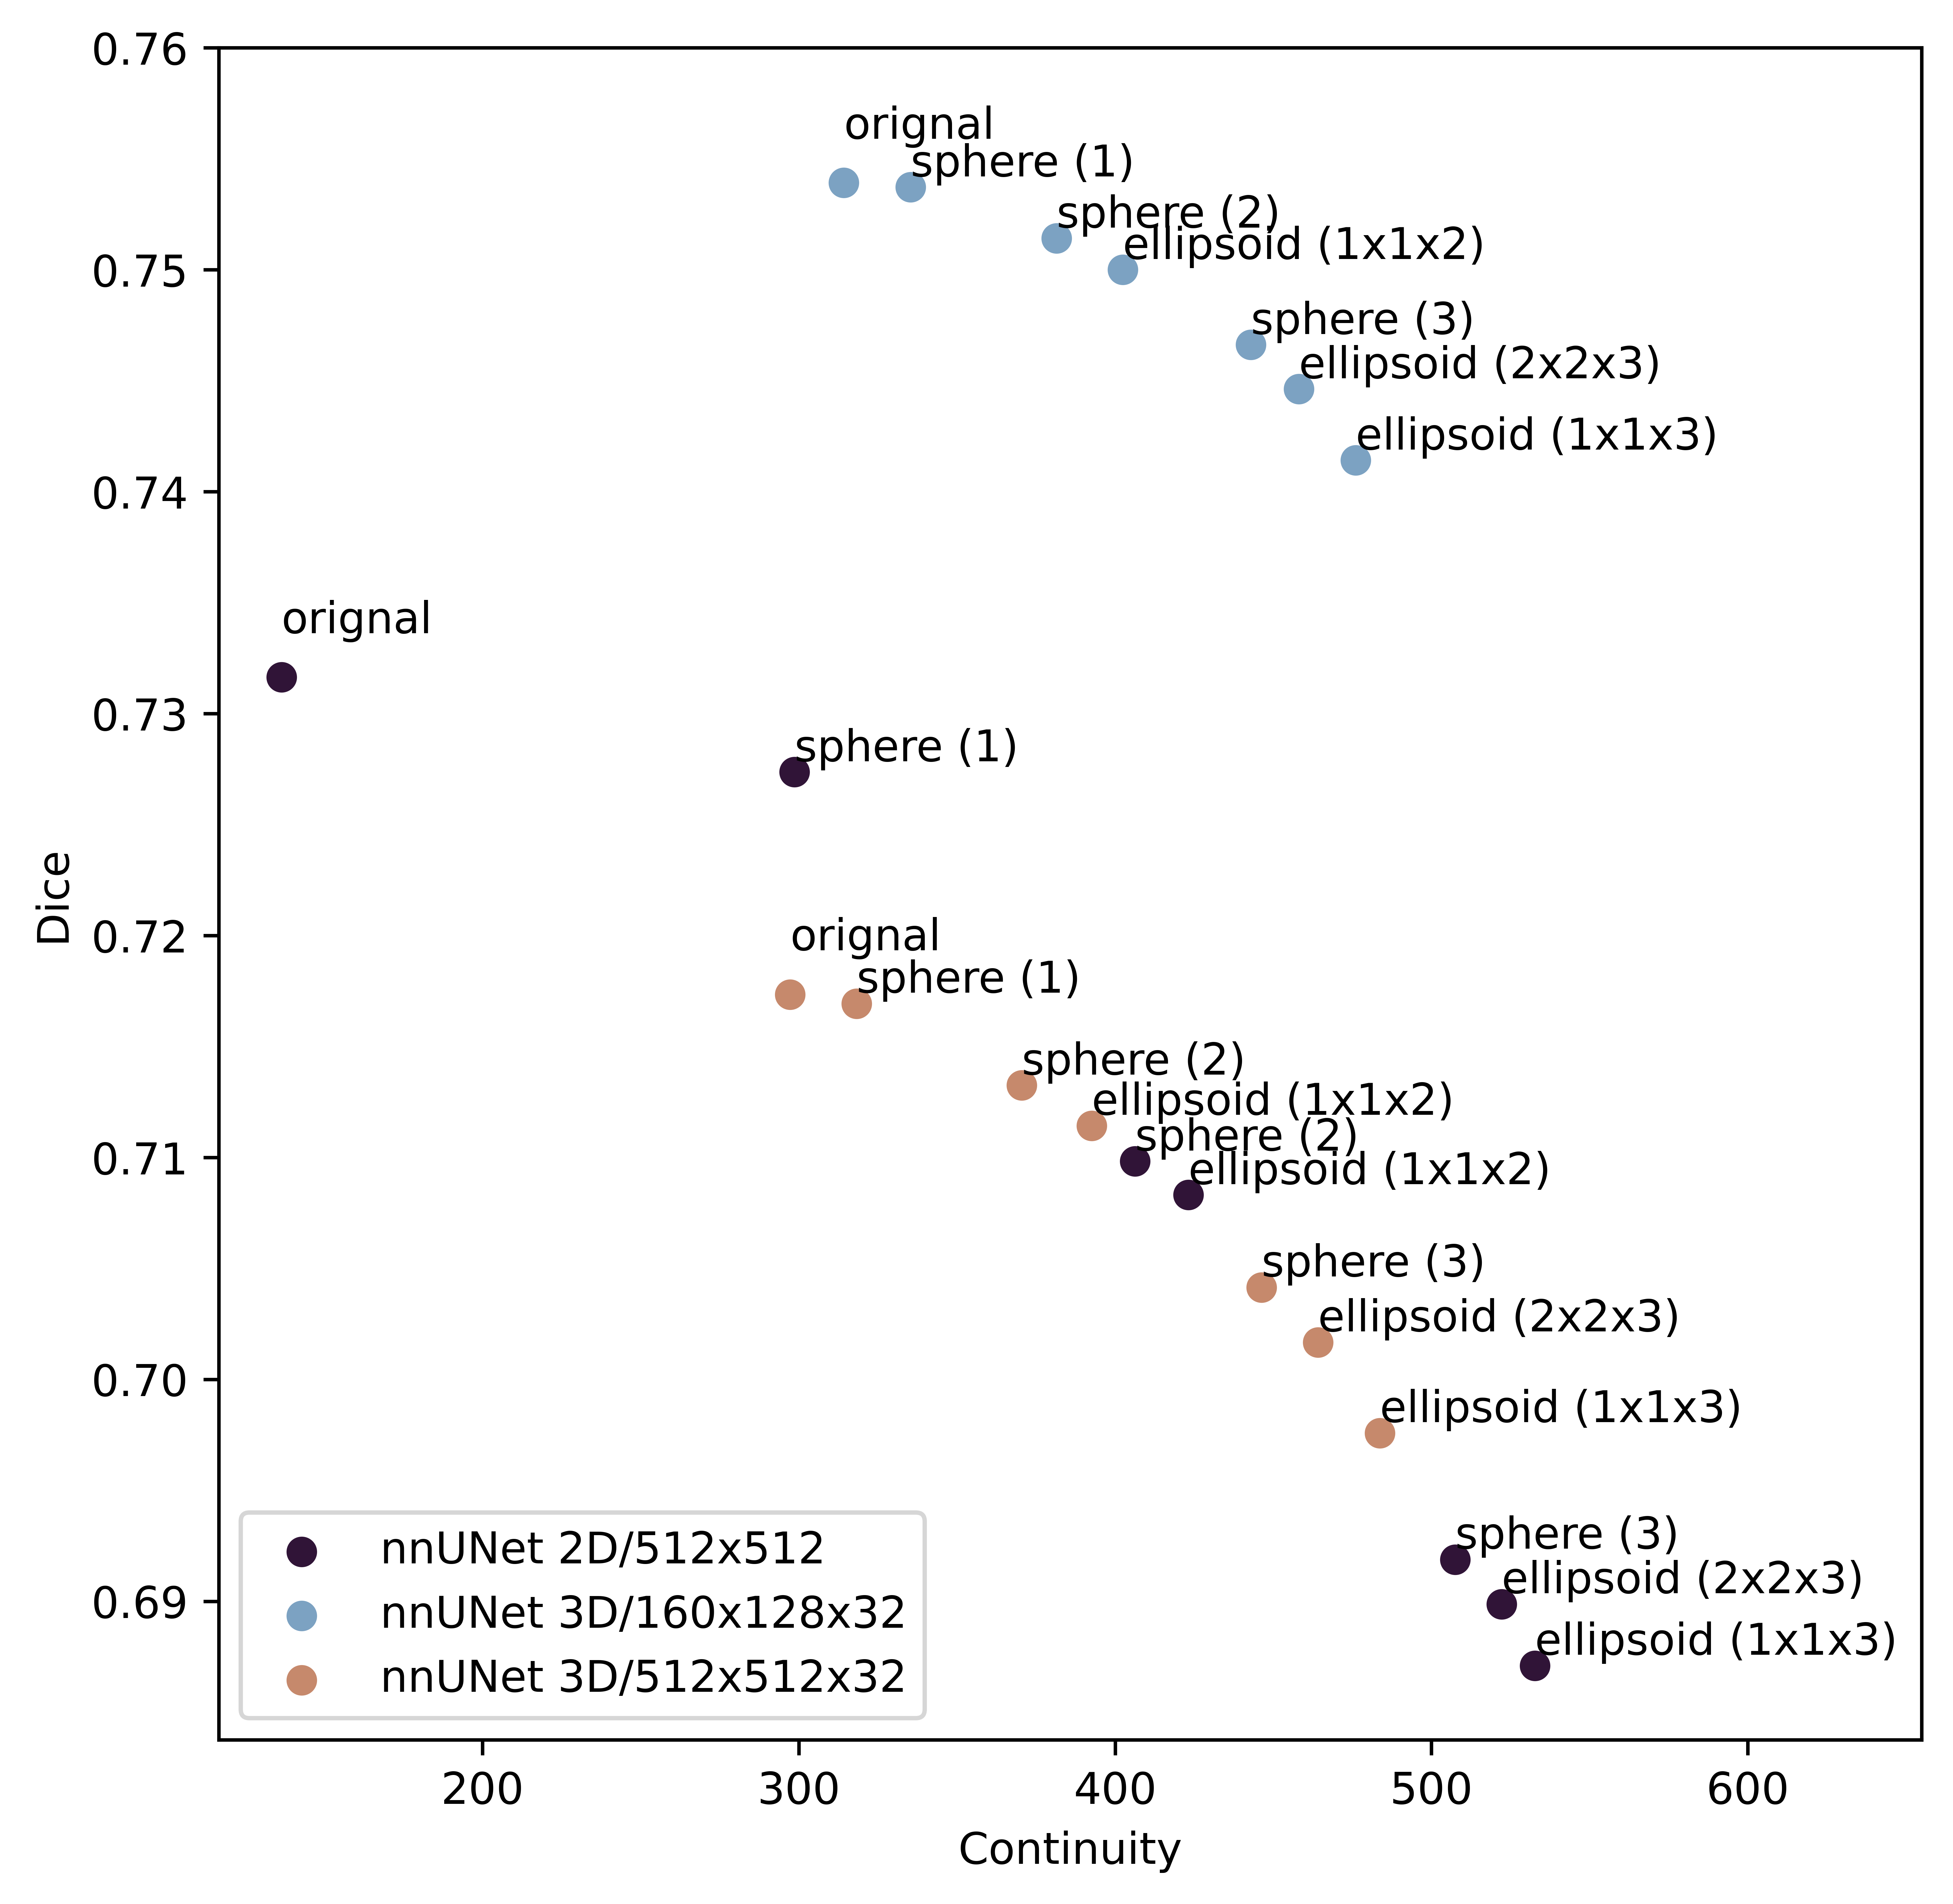
\includegraphics[width=0.5\linewidth]{figures/result_nnunet_dice_and_continuity.png}
    \caption{A plot showing the relationship between Dice score and continuity as smoothing is increasingly applied. Original denotes the initial segmentation. Each point is annotated with the kernel shape and size ($H\times W\times D$) used in smoothing.}
    \label{fig:nnunet-continuity-vs-correctness}
\end{figure}

Correctness (represented by Dice score) and continuity were examined in 3 models: 2D $512\times 512$, 3D $160\times 128\times 32$, and 3D $512\times 512\times 32$, with results illustrated in Figure~\ref{fig:nnunet-continuity-vs-correctness}. The original segmentation of all models began in the top left extreme. As the models underwent smoothing with kernels of various shapes and sizes, segmentation became more continuous at the expense of correctness. The extent of this trade-off varied across the 3 models, but 3D nnUNet showed a smaller trade-off than 2D nnUNet as evidenced by a more gradual descending slope. Therefore, 3D segmentation may be advantageous over 2D segmentation when continuity is required.

\subsection{SuPreM}
We evaluated three configurations of the SwinUNETR model as described in Section~\ref{sec:design:suprem}. SwinUNETR denotes a model trained from scratch on Calcium OCT; SwinUNETR (SSL) denotes a self-supervised SwinUNETR model fine-tuned on Calcium OCT; and SwinUNETR (SuPreM) denotes a SuPreM-pre-trained model fine-tuned on Calcium OCT. The results are summarized in Figure~\ref{fig:suprem-results}. 

SuPreM pre-trained SwinUNETR yielded the best results with an average Dice score of $0.631\pm0.030$, which was statistically higher than those of the other two configurations. However, even the top-performing SuPreM configuration still vastly underperformed 2D nnUNet ($0.631$ versus $0.753$; Figure~\ref{fig:transformer-results}). More discussion is provided in the next section. %SuPreM pre-training provides superior features for calcium segmentation compared to self-supervised learning and training from scratch. 

\begin{figure}[hbt]
    \centering
    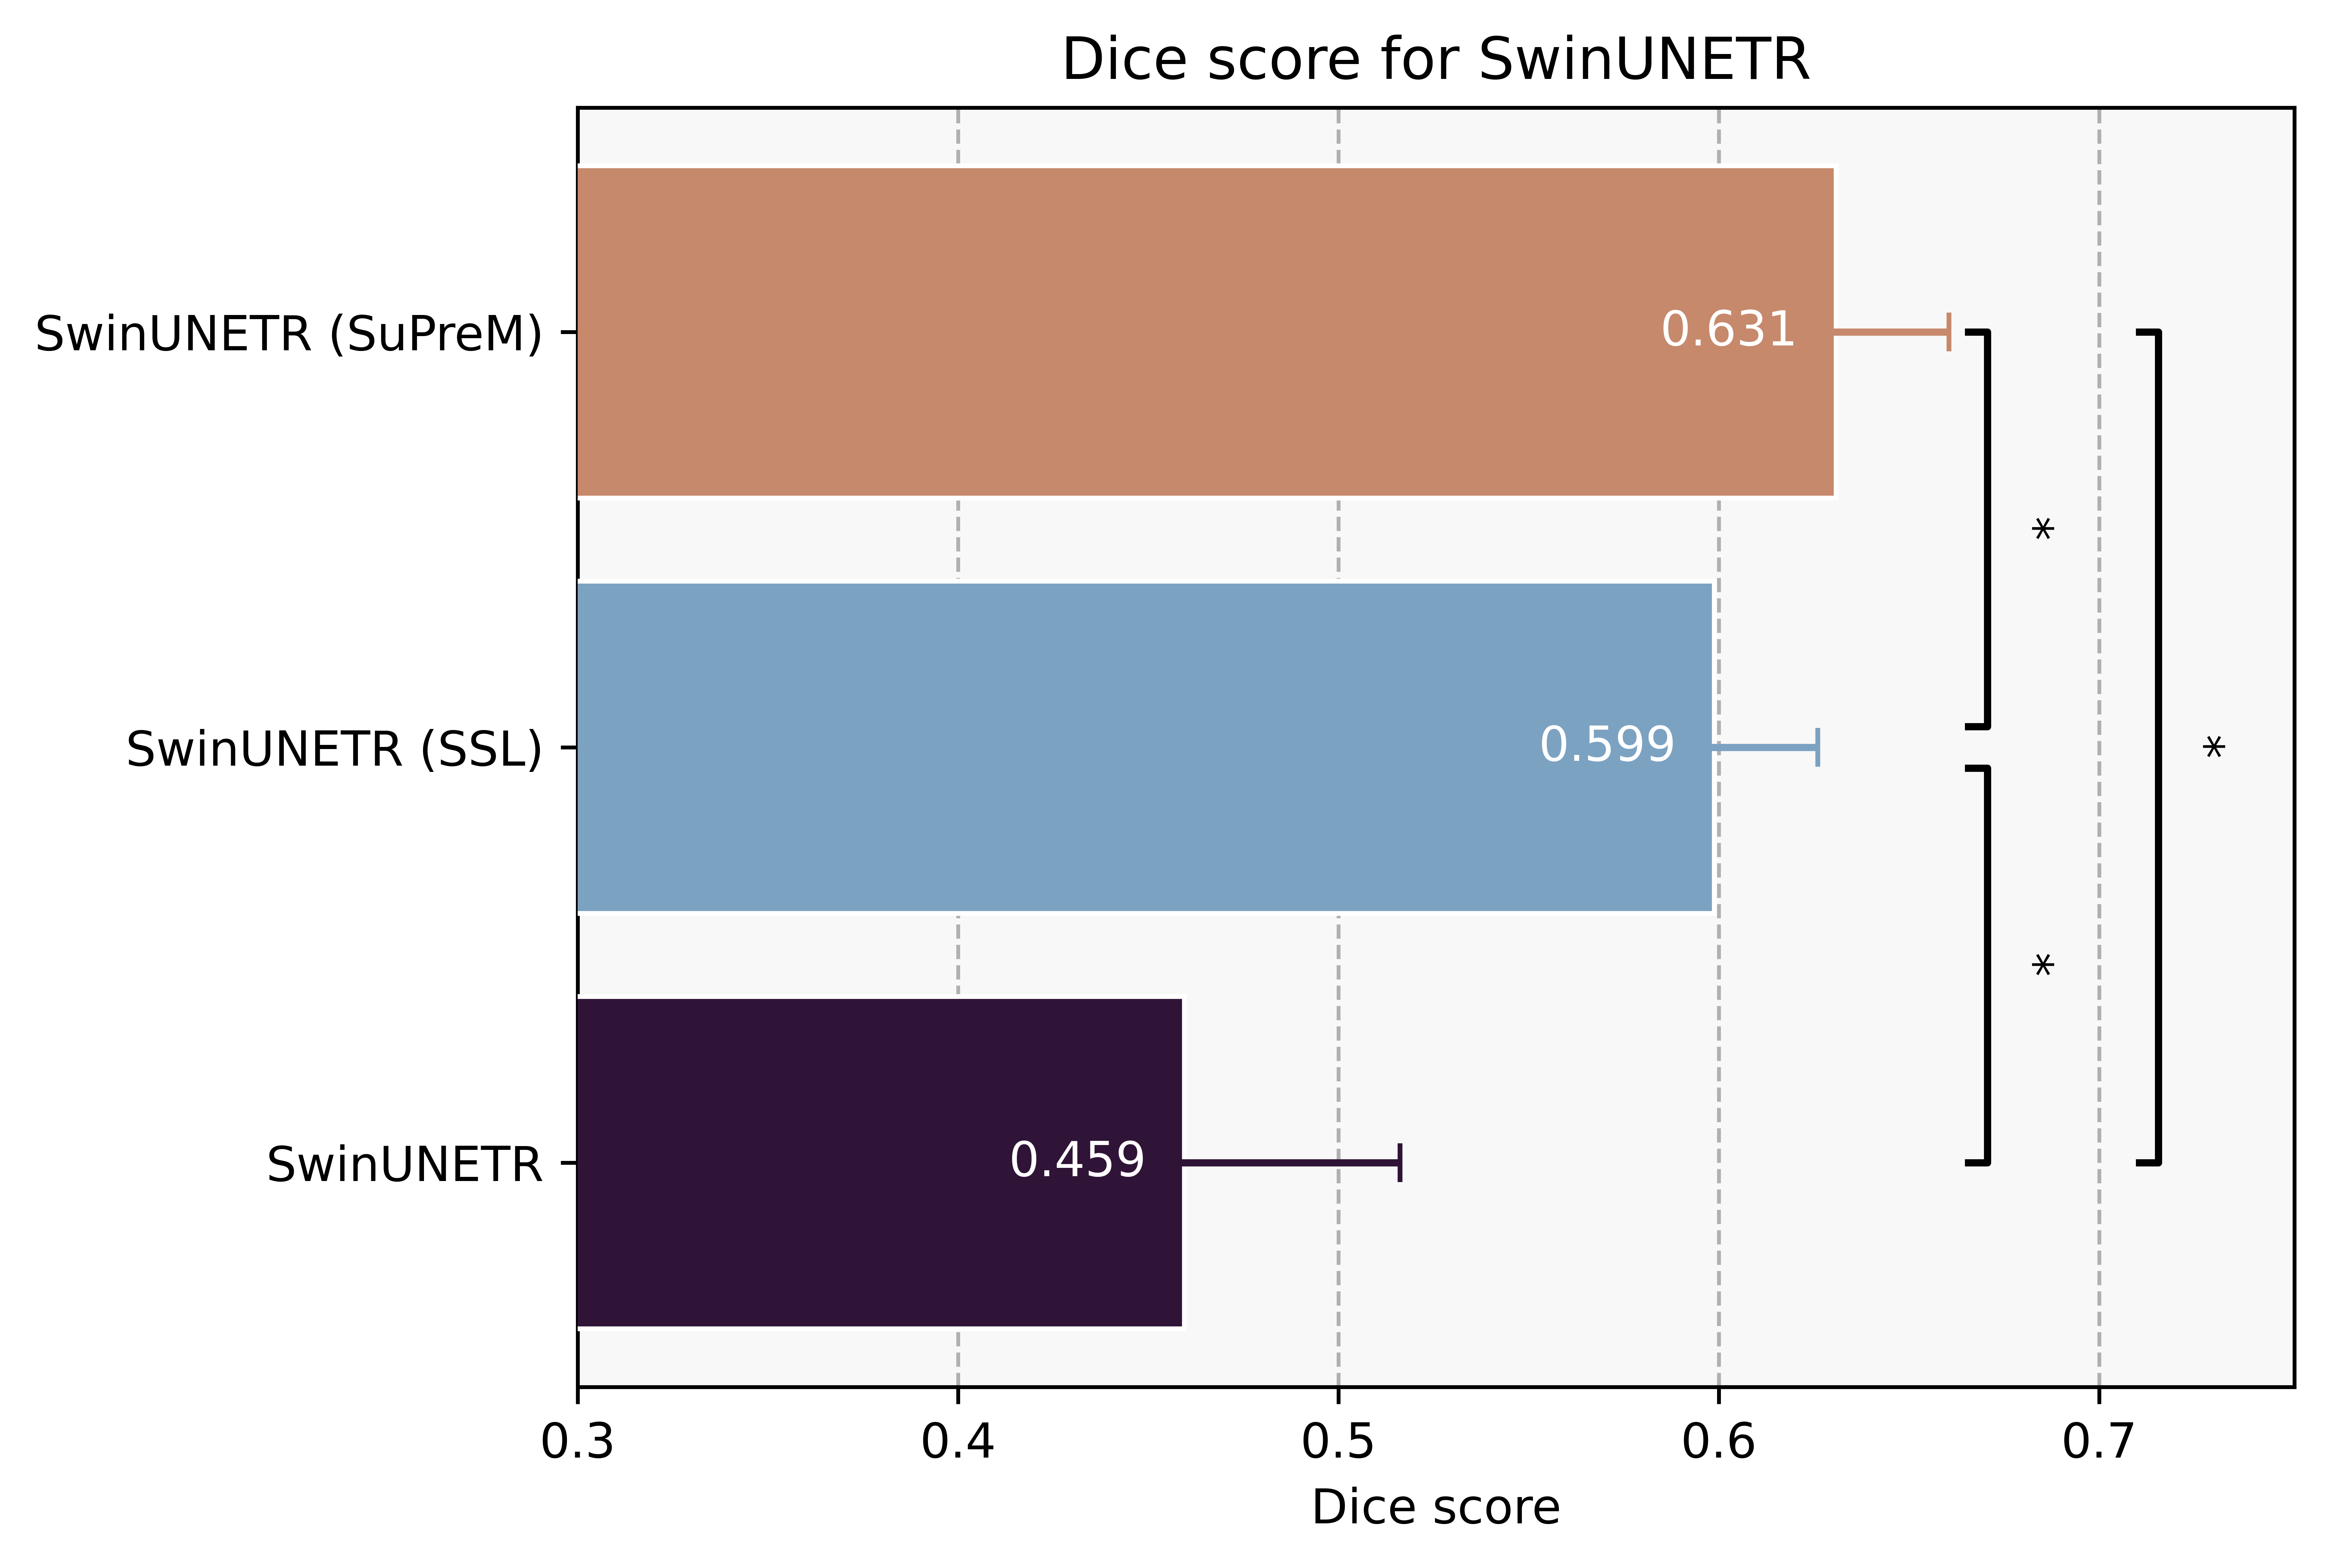
\includegraphics[width=0.5\linewidth]{figures/result_SwinUNETR_results.png}
    \caption{Dice scores of SwinUNETR models. Parentheses indicate pre-training algorithms. SuPreM pre-training on SwinUNETR (SwinUNETR (SuPreM)) yielded the best results and was significantly better than both self-supervised pre-training (SwinUNET (SSL)) and training from scratch (SwinUNETR).}
    \label{fig:suprem-results}
\end{figure}

%However, when comparing the result of the SuPreM pre-trained SwinUNTER model with that of the best 2D nnUNet model, the 2D nnUNet model outperforms the SuPreM model (see Figure~\ref{fig:transformer-results}). This will be discussed in the next section.

\subsection{SegFormer and RADIO}
SegFormer (ADE60K) and RADIO gave average Dice scores of 0.687 and 0.543, respectively, which significantly underperformed the best 3D nnUNet model (0.742) (Figure~\ref{fig:transformer-results}). This might be because nnUNet was designed specifically for small-scale datasets, which is more suitable for our context.
% This may be attributed to fundamental differences between CNN and transformer architectures. CNNs are designed to learn local features, while transformers are designed to learn global features.
% Calcium plaques in OCT images are localized, making CNNs more suitable for this task. This is also supported by the fact that, in CNNs, increasing the patch size in the width and height dimensions of the 3D nnUNet does not improve performance, while reducing the patch size in the depth dimension significantly improves performance (see Section~\ref{sec:result:nnunet}). The effectiveness of the SegFormer, ViT (RADIO), and SwinUNTER (SuPreM) compared to the nnUNet is summarized in Figure~\ref{fig:transformer-results}.

\begin{figure}[hbt]
    \centering
    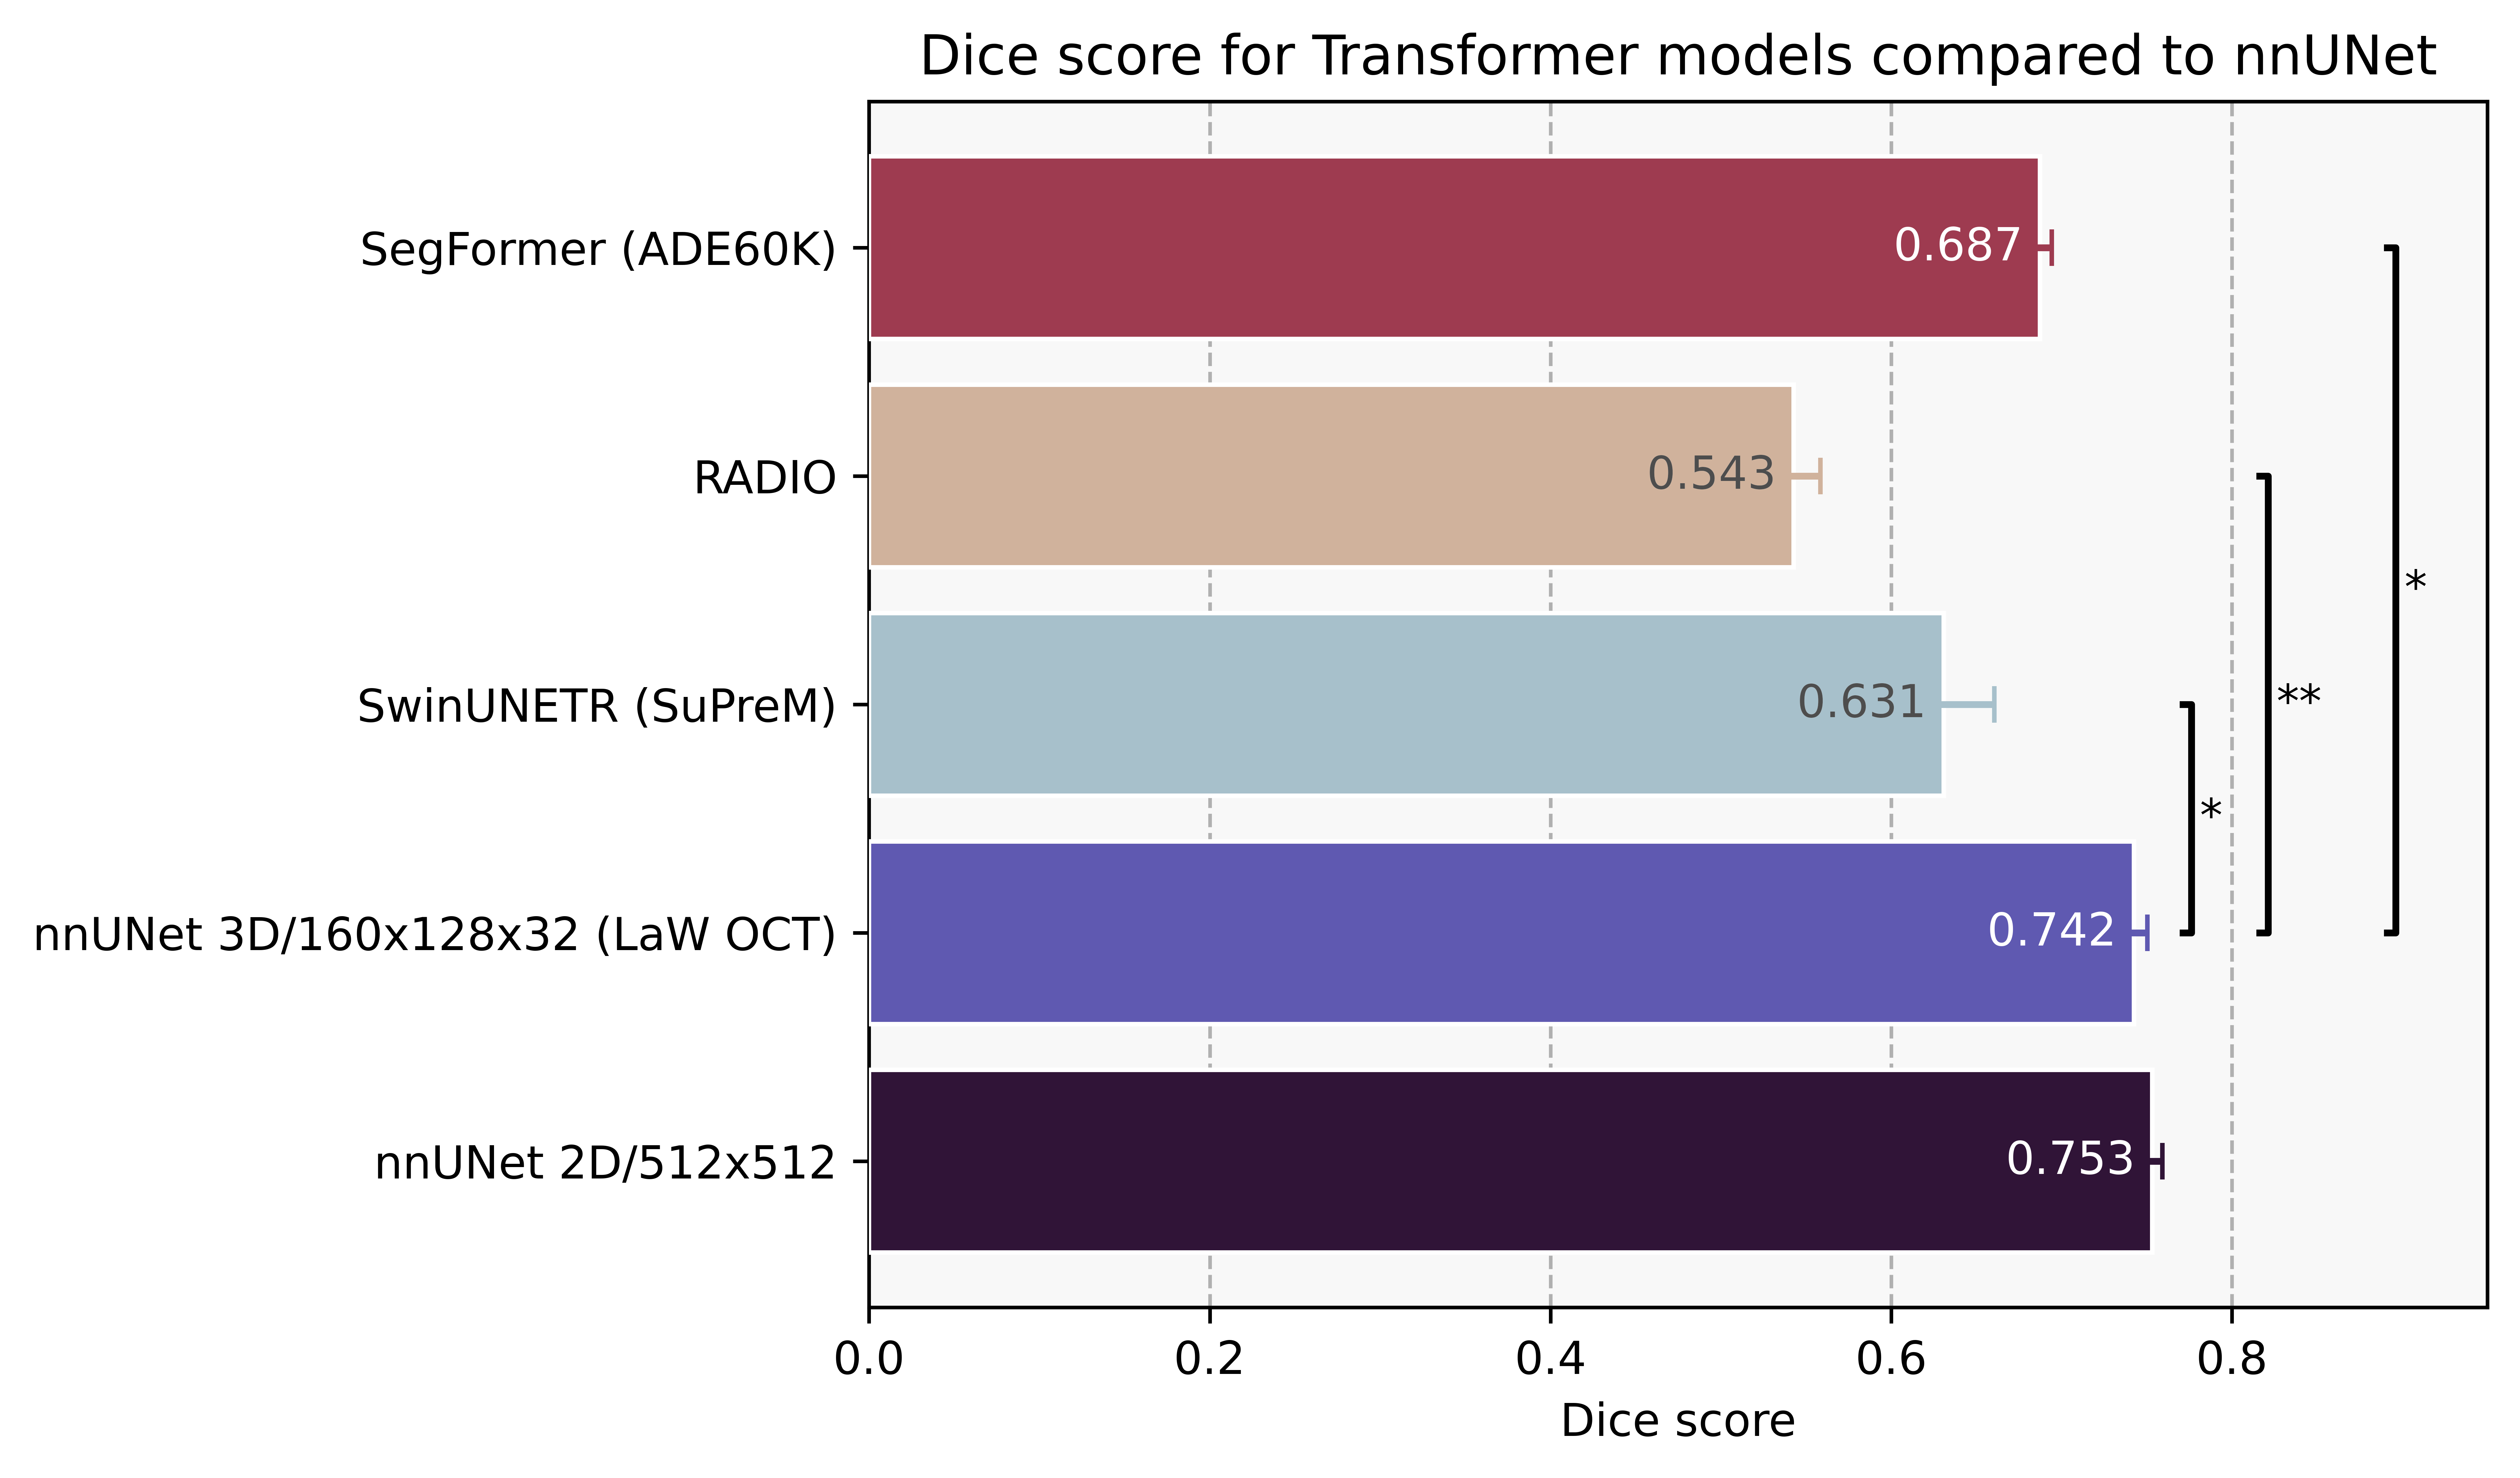
\includegraphics[width=0.6\linewidth]{figures/result_nnUNet_vs_Transformer_results.png}
    \caption{Dice scores of transformer-based models compared to those of the nnUNet. Compared to the best 3D nnUNet model pre-trained on the LaW OCT dataset, Dice scores of transformer-based models are significantly lower.}
    \label{fig:transformer-results}
\end{figure}

\section{Supervised Learning}
\subsection{V-JEPA}
Many variations of V-JEPA were conducted, and they were named based on the following nomenclature: "architecture + decoder head (dataset used for V-JEPA pre-training)". For example, "ViT+Attentive (V-JEPA VideoMix2M)" denotes the ViT architecture with an attentive decoder head pre-trained on the VideoMix2M dataset. Results are summarized in Figure~\ref{fig:vjepa-decoder-results}. The control experiment, \textbf{ViT + Attentive*} without V-JEPA pre-training, gave a Dice score of 0.316 as the baseline for comparison. 

\subsubsection{Effect of Pre-training}
\textbf{ViT + Attentive* (V-JEPA VideoMix2M)} significantly improved the performance of the ViT model compared to the no-pretraining control (\textbf{ViT + Attentive*}) (Dice scores = 0.672 versus 0.316; Figure~\ref{fig:vjepa-decoder-results}). This observation suggests that the representation learned by V-JEPA on VideoMix2M is useful for calcium segmentation and highlights the utility of V-JEPA pre-training. 

Even though V-JEPA pre-trained on VideoMix2M yielded a significant improvement over the baseline, V-JEPA pre-trained on our unannotated OCT images \textbf{ViT + Attentive* (V-JEPA Unannotated OCT)} did not improve the performance of the ViT model over the baseline (Dice scores = 0.320 versus 0.316; Figure~\ref{fig:vjepa-decoder-results}). The difference in these outcomes may be related to dataset size. Unannotated OCT consists of only 500 volumes, whereas VideoMix2M contains 2 million videos. This demonstrates the importance of dataset scale for self-supervised learning on transformer-based models.

\subsubsection{Effect of Decoder Head}
There was no significant difference between the various decoder heads (Attentive, Attentive*, Multifeat, and BNLinear). All of these decoders gave similar Dice scores ranging from 0.653 to 0.672 when used with ViT and V-JEPA pre-trained with VideoMix2M.

\subsubsection{Comparison to nnUNet}
The best V-JEPA model pre-trained on VideoMix2M, \textbf{ViT + Attentive* (V-JEPA VideoMix2M)}, was significantly worse than 3D nnUNet pre-trained on LaW OCT ($0.672$ versus $0.742$). This may be due to a domain shift between natural and medical images. Had the V-JEPA model been pre-trained on a larger unannotated dataset, the results might have been comparable.

\begin{figure}[hbt]
    \centering
    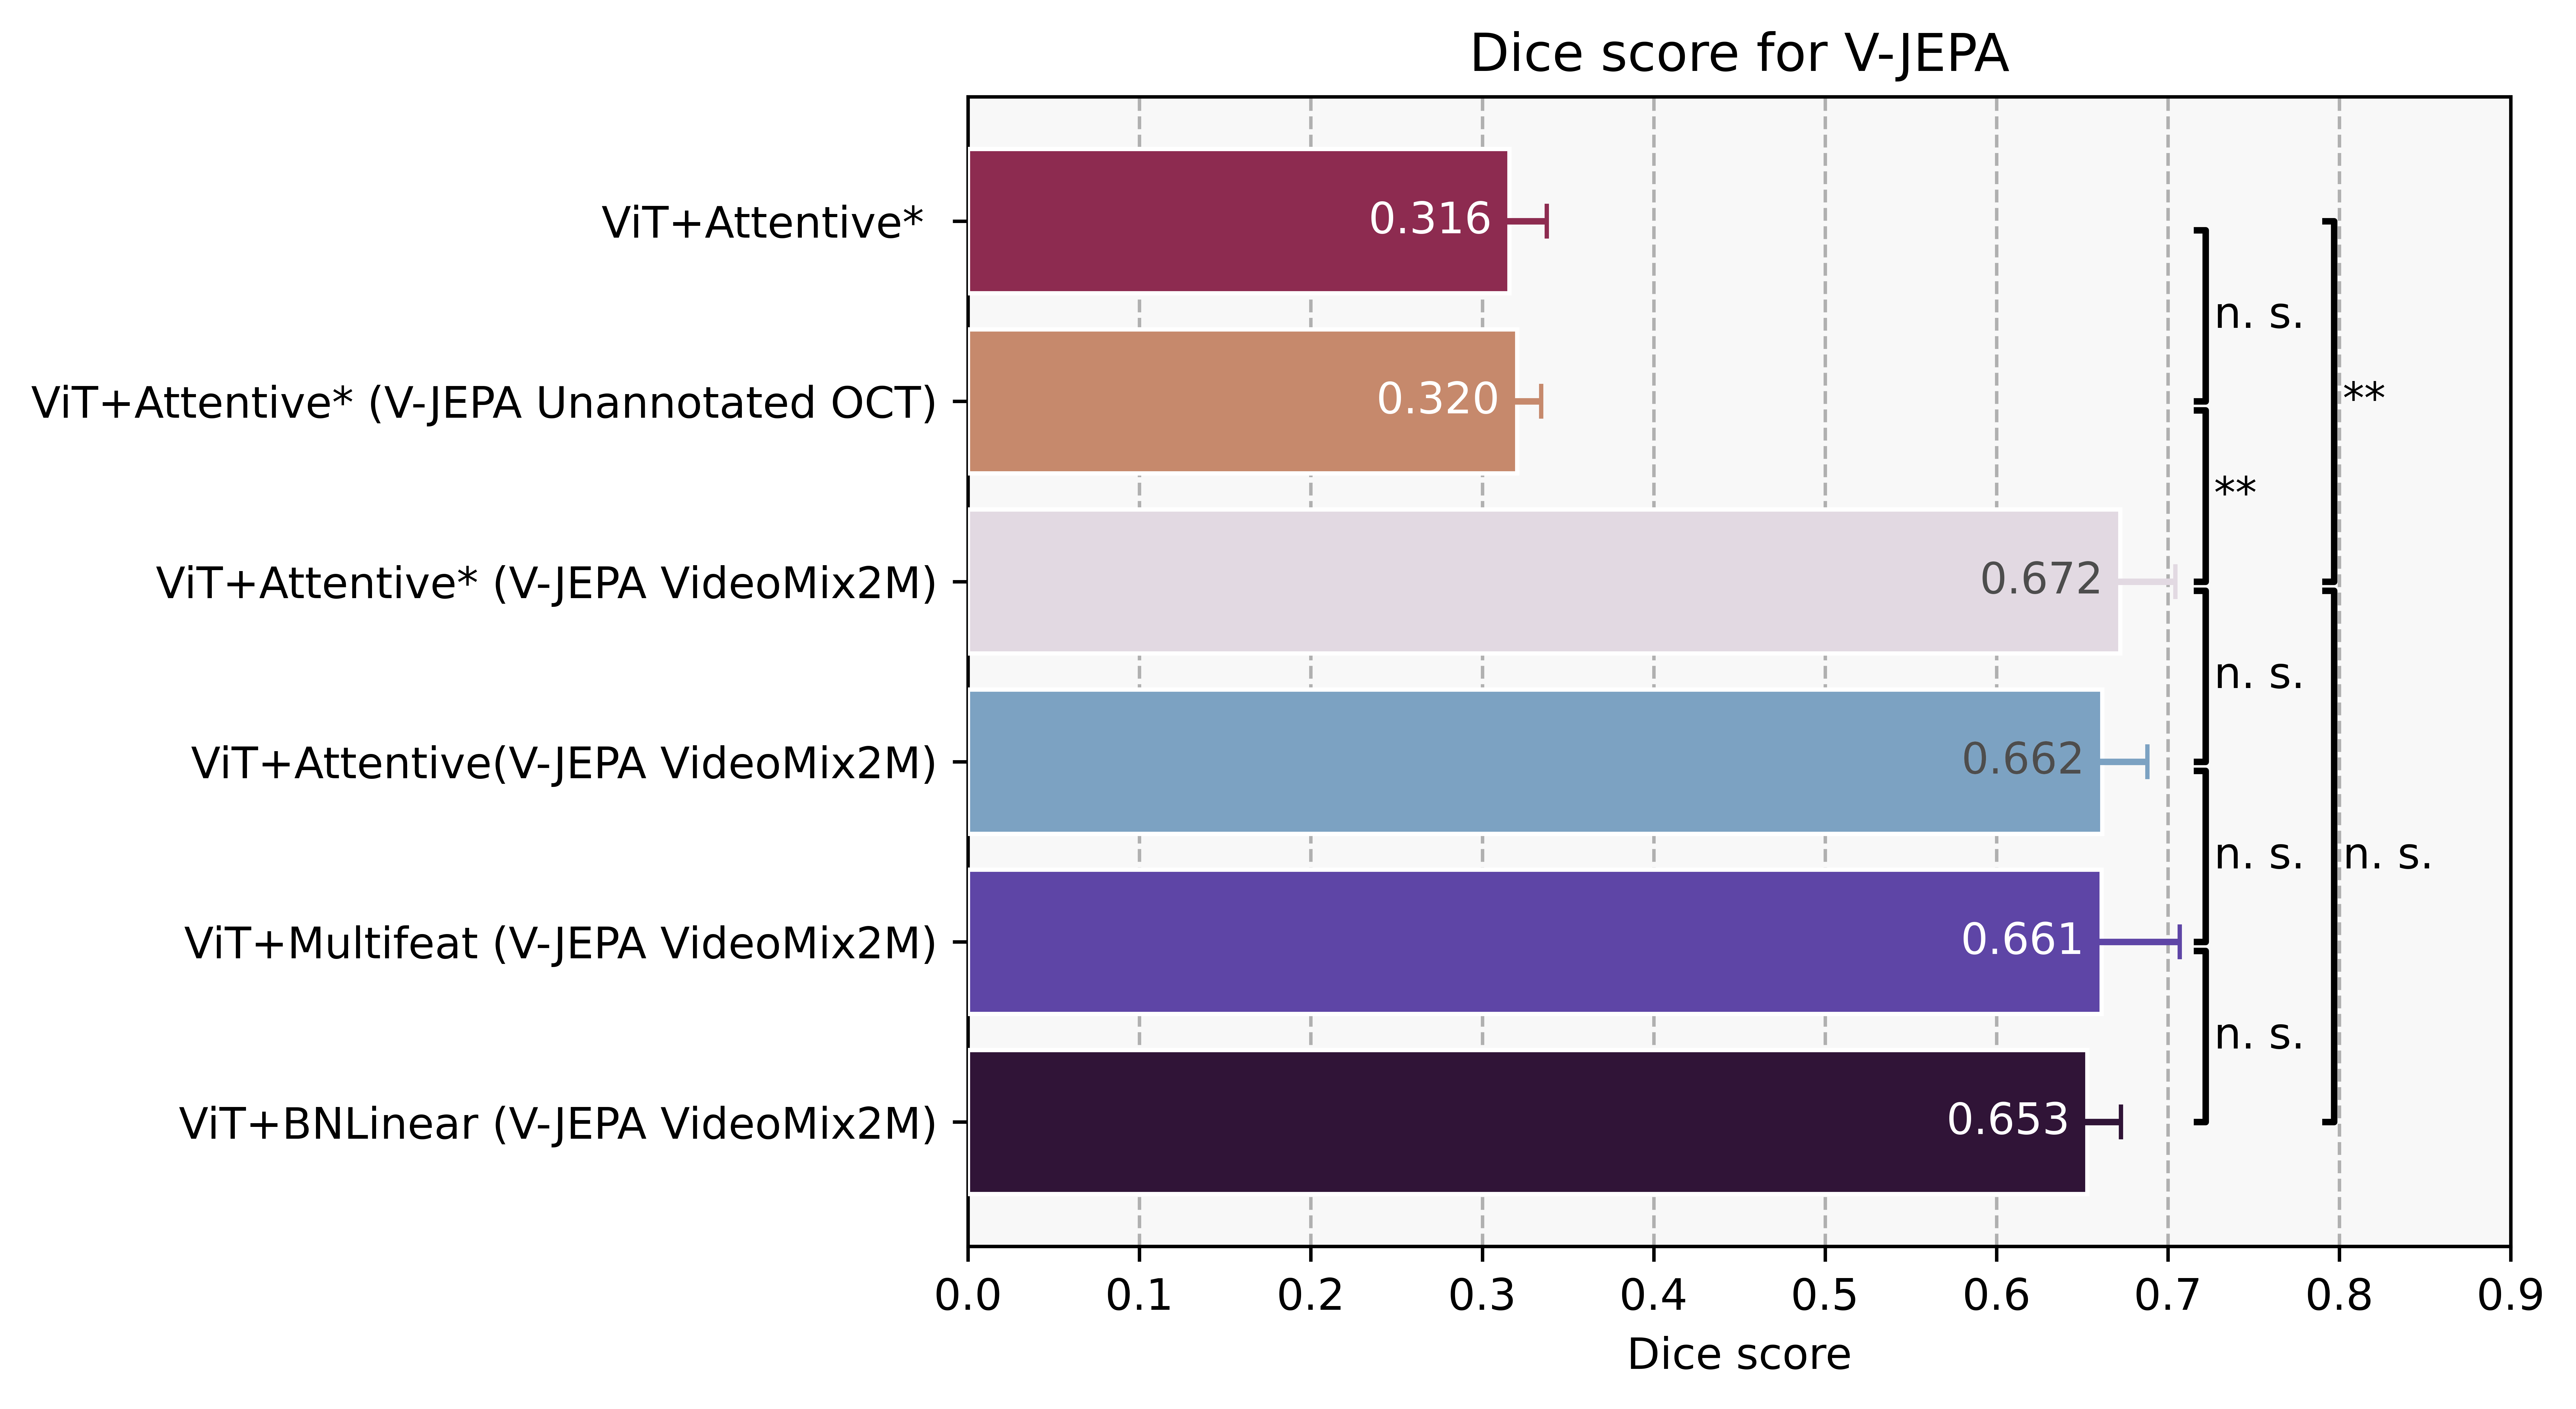
\includegraphics[width=0.75\linewidth]{figures/result_VJEPA_results.png}
    \caption{Dice score of V-JEPA algorithms with various decoder heads and pre-trained datasets. BNLinear denotes batch normalization followed by linear projection. Attentive signifies the attentive decoder head. Attentive* indicates an attentive decoder head with more intensive data augmentation and positive data sampling. MultiFeat denotes the multi-features decoder head. The dataset used to pre-train V-JEPA is indicated in parentheses.}
    \label{fig:vjepa-decoder-results}
\end{figure}


\subsection{CLIP}
CLIP pre-training on co-registered Pre-IVL/Post-IVL OCT images (0.744) provided a small yet statistically significant improvement in performance over the baseline 3D nnUNet model (0.732) and was on par with the 3D nnUNet model pre-trained on the LaW OCT dataset (0.742) (Figure~\ref{fig:clip-results}). 

The similarity in effectiveness between CLIP and nnUNet models is particularly remarkable because the former is semi-self-supervised whereas the latter is fully supervised. This result demonstrates that it is possible to achieve comparable performance while paying a much lower cost of co-registering Pre-IVL/Post-IVL images for CLIP than annotating the lumen and wall for nnUNet, further supporting the promise of SSL for image segmentation.% while the cost for co-registration is lower than the cost for annotating the lumen and wall. The performance of CLIP pre-training on co-registered multi-modal OCT images is summarized in Figure~\ref{fig:clip-results}.

\begin{figure}[h]
    \centering
    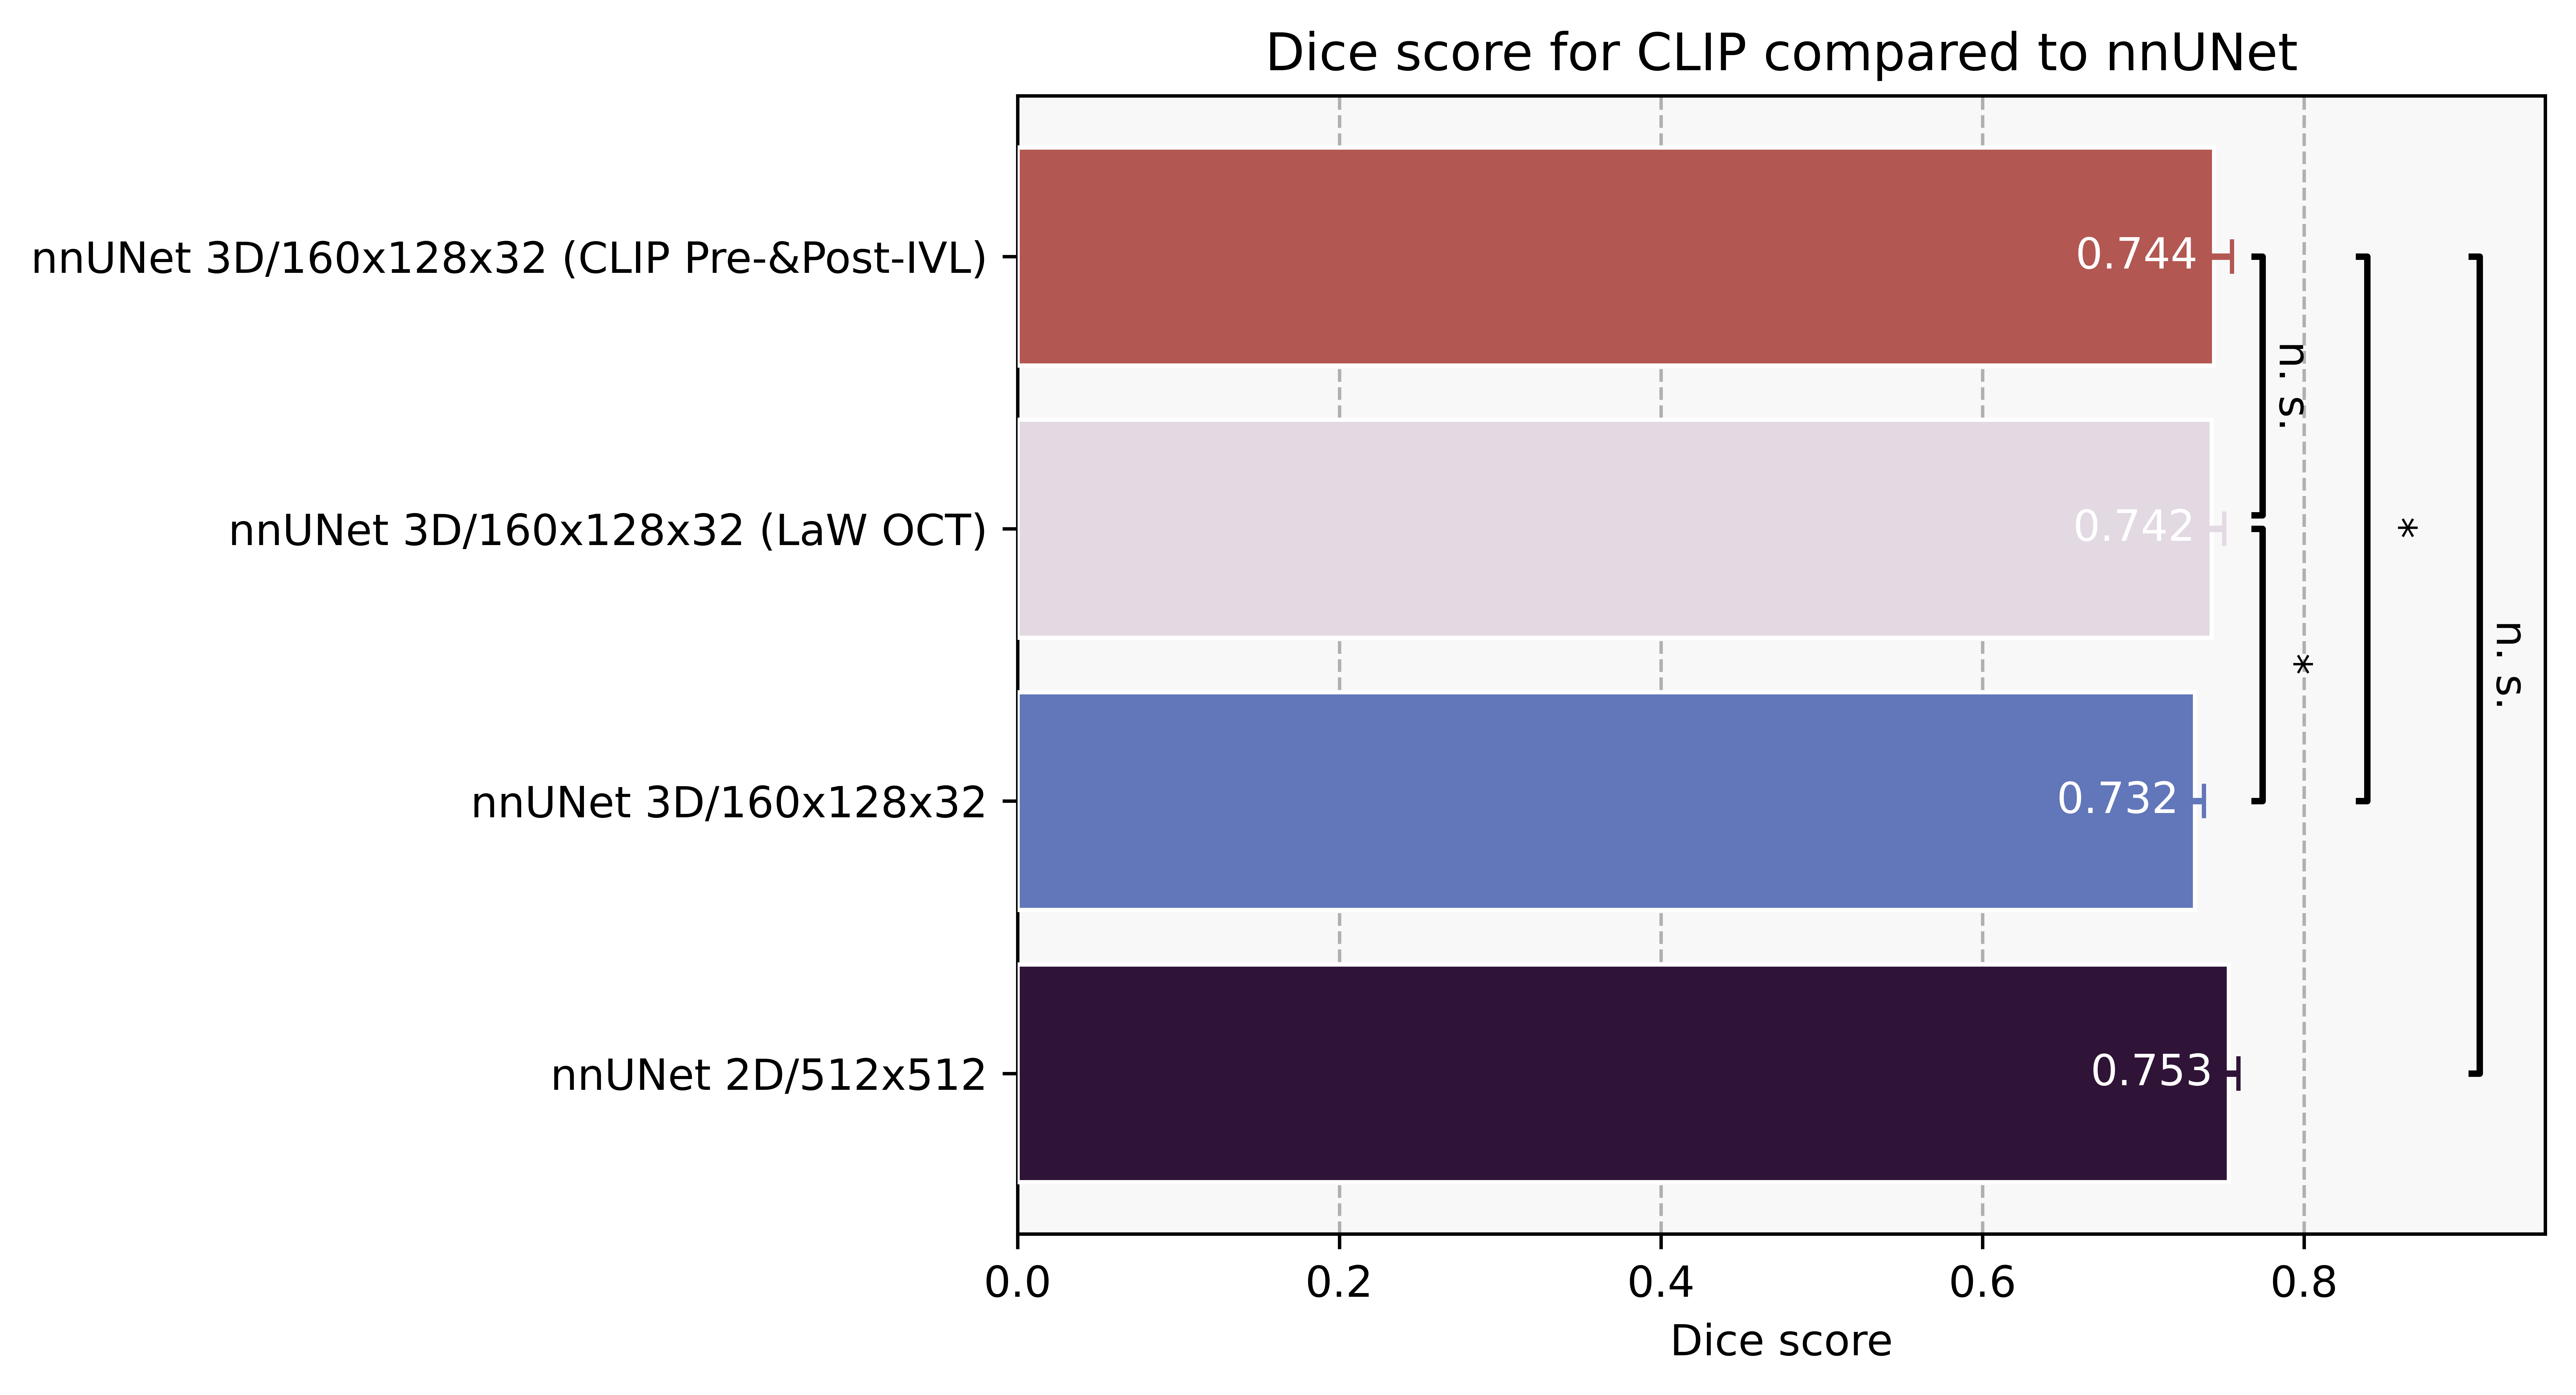
\includegraphics[width=0.65\linewidth]{figures/result_nnUNet_and_CLIP_results.png}
    \caption{Dice scores of CLIP on the Calcium OCT dataset compared to nnUNet. The algorithm and dataset used for pre-training are indicated in parentheses. LaW OCT denotes the Lumen and Wall OCT dataset. CLIP denotes pre-training on co-registered Pre-IVL and Post-IVL images.
    }
    \label{fig:clip-results}
\end{figure}

The success of CLIP pre-training may result from the fact that aligning Pre-IVL and Post-IVL images requires the model to learn the features of the lumen and wall, which has been proven to be useful for calcium segmentation in 3D nnUNet as described in the previous section. In other words, CLIP (Pre-IVL/Post-IVL) and LaW OCT possibly teach the model similar knowledge in identifying the arterial lumen and wall, giving rise to similar calcium segmentation performances. To support this hypothesis, we performed a principal component analysis (PCA) of the features learned by CLIP compared to the features output from the initial weight of the model and confirmed that CLIP indeed was better at distinguishing the details of the arterial wall.

\begin{figure}[h]
    \centering
    \begin{subfigure}[t]{0.5\textwidth}
        \centering
        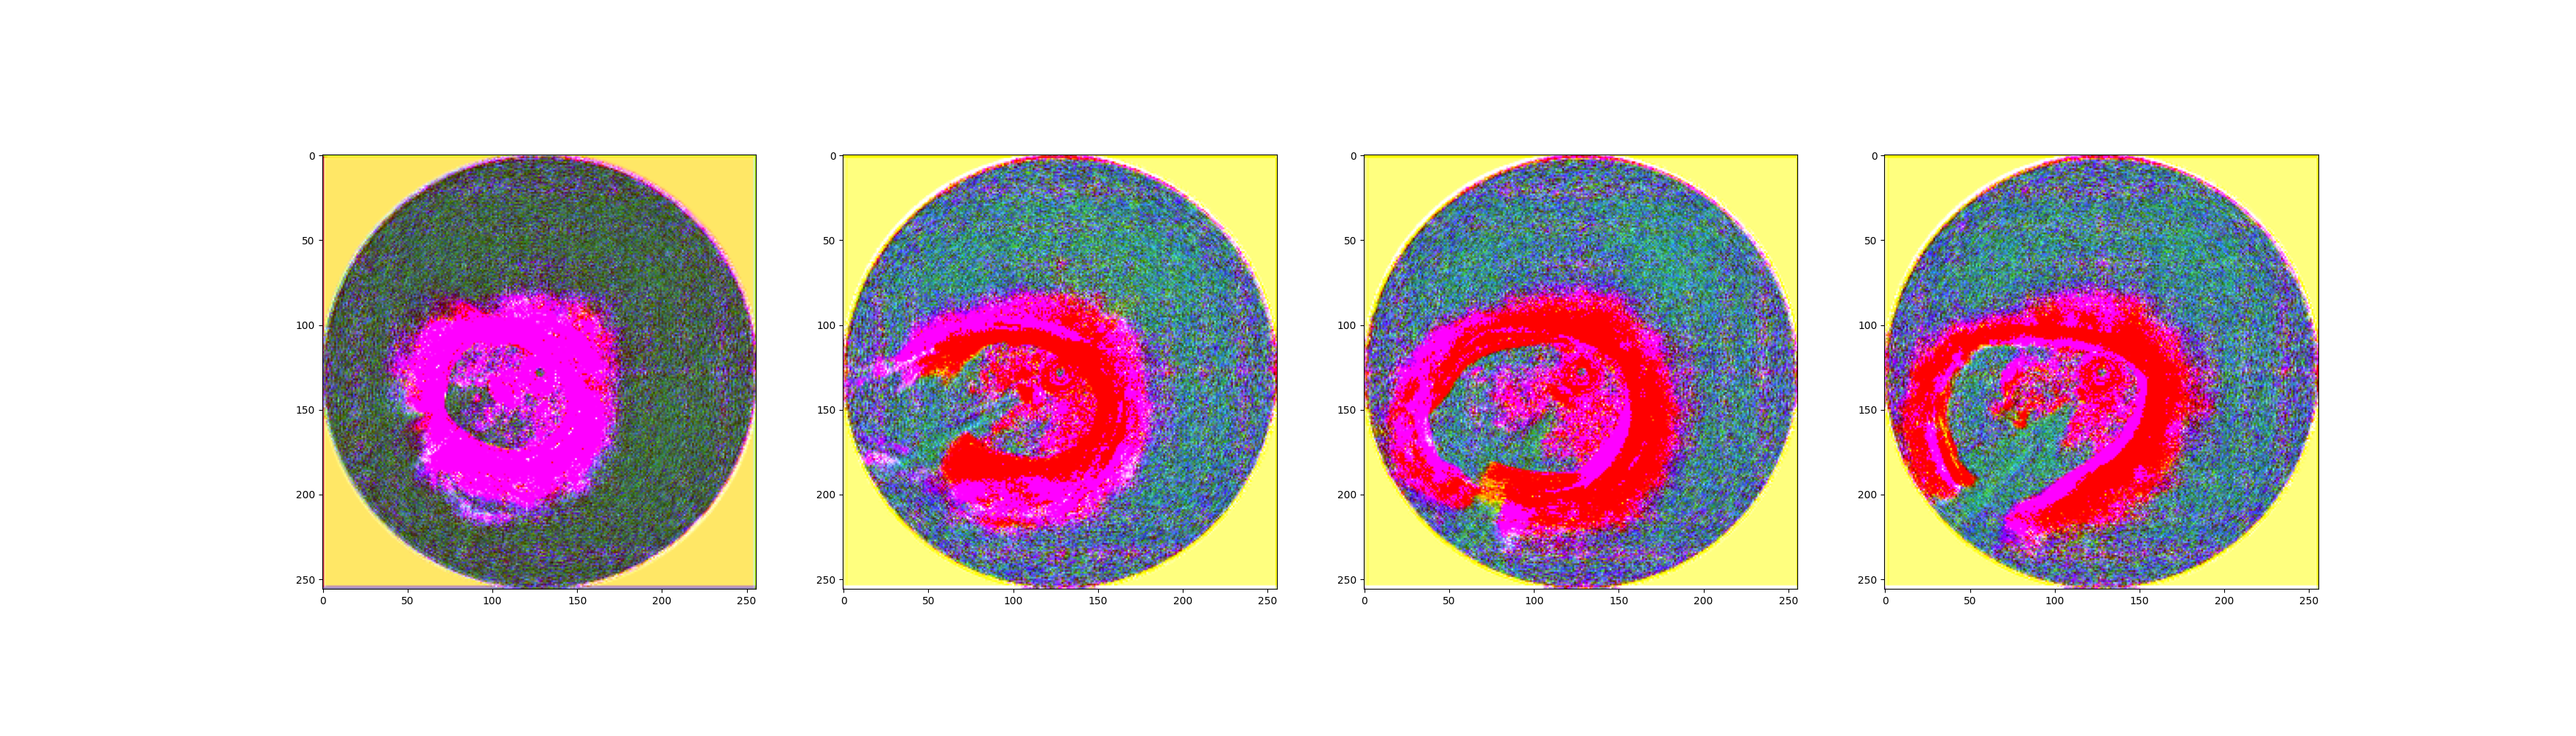
\includegraphics[width=\linewidth]{figures/discussion_default_feature_map_batch0_feature1.png}
        \caption{PCA of the output of the features from the initial weight of the model.}
        \label{fig:pca-initial}
    \end{subfigure}%
    \begin{subfigure}[t]{0.5\textwidth}
        \centering
        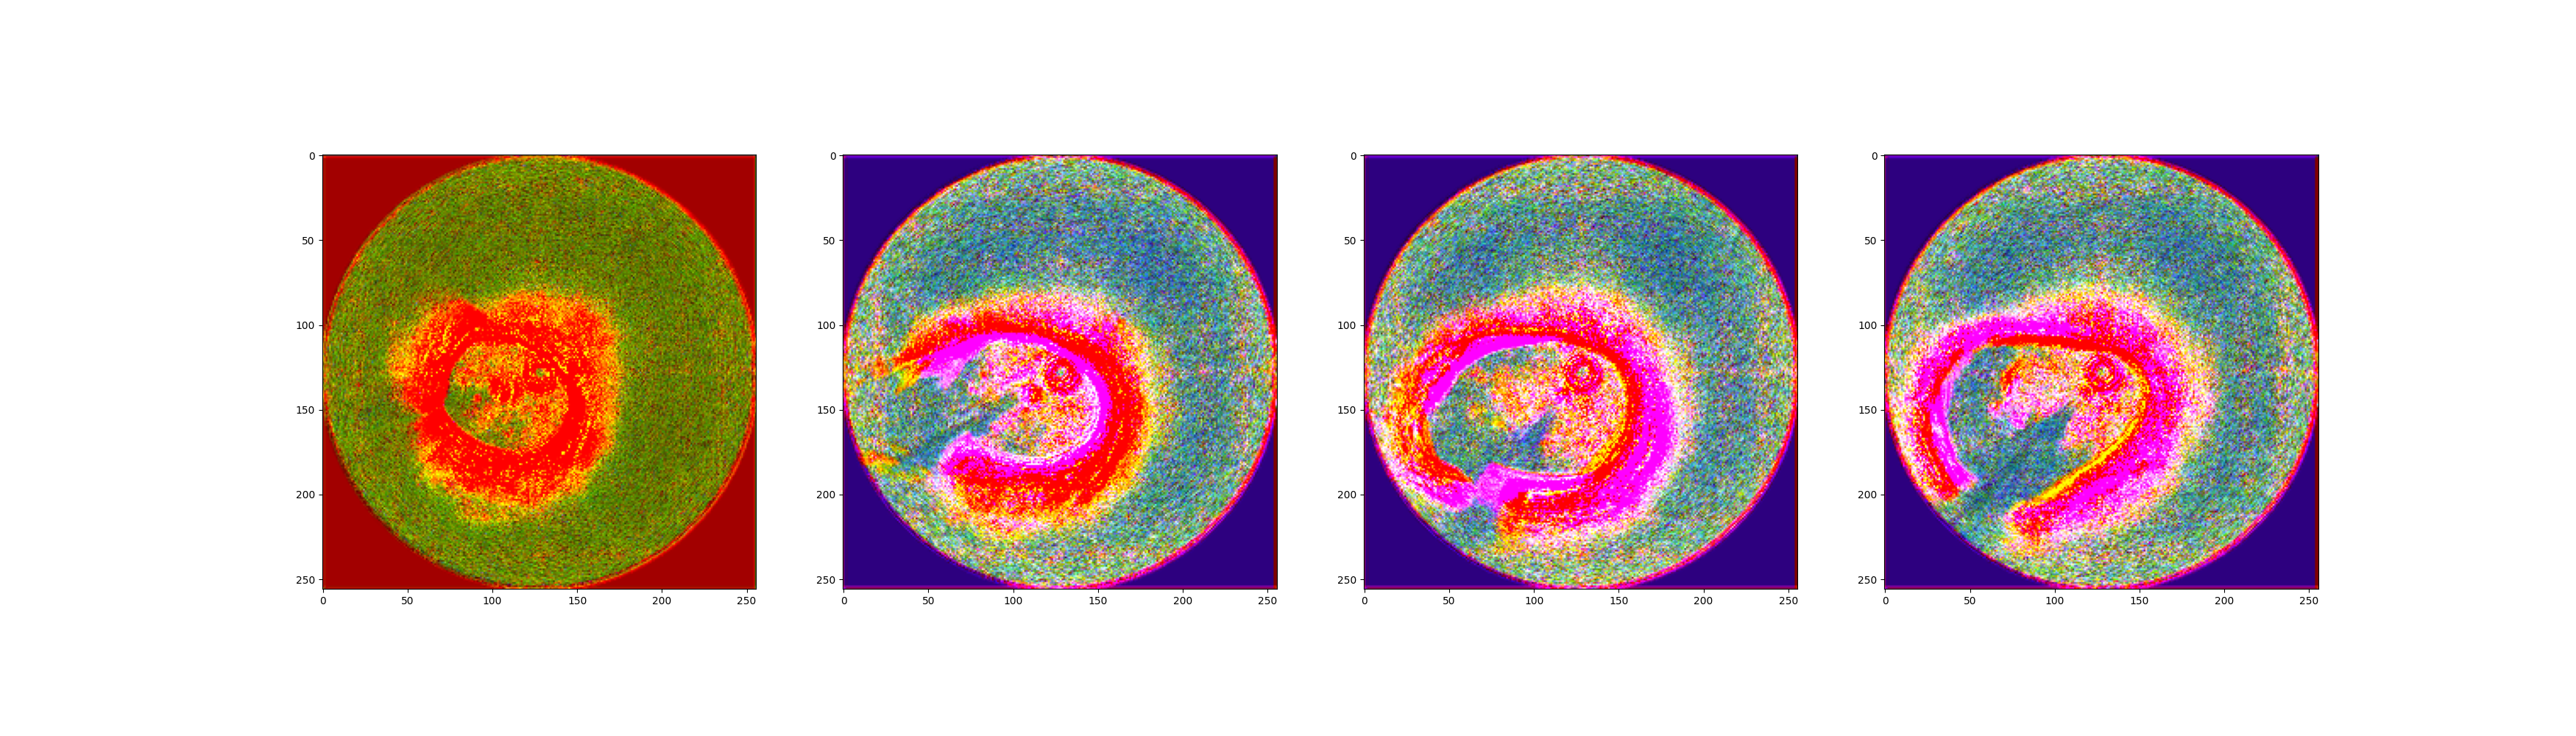
\includegraphics[width=\linewidth]{figures/discussion_clip_feature_map_batch0_feature1.png}
        \caption{PCA of the features learned by CLIP.}
        \label{fig:pca-clip}
        
    \end{subfigure}
    \caption{PCA of the output of the features from the initial weight of the model and the features learned by CLIP. CLIP pre-training provides more distinguishable features of the walls than those from the initial weight of the model. 
    }
\end{figure}

The dataset used for CLIP in our study includes co-registered Pre-IVL and Post-IVL images. We suggest that similar experiments be further studied on co-registered Pre-IVL and Post-Stent images, which are also available from our unannotated OCT dataset, as this may achieve comparable if not greater performance.

\subsection{Genesis}
Pre-training Genesis on unannotated OCT images resulted in a Dice score of $0.744\pm0.000$. Genesis provided a small yet statistically significant improvement over 3D nnUNet (0.732), performing comparably to the best 2D nnUNet (0.753) and the 3D nnUNet pre-trained on the LaW OCT dataset (0.742). Again, this similarity in performance between Genesis and nnUNet is particularly remarkable, considering that Genesis requires no data annotations while supervised pre-trained nnUNet does. The results and statistical tests are summarized in Figure~\ref{fig:genesis-results}.

\begin{figure}[h]
    \centering
    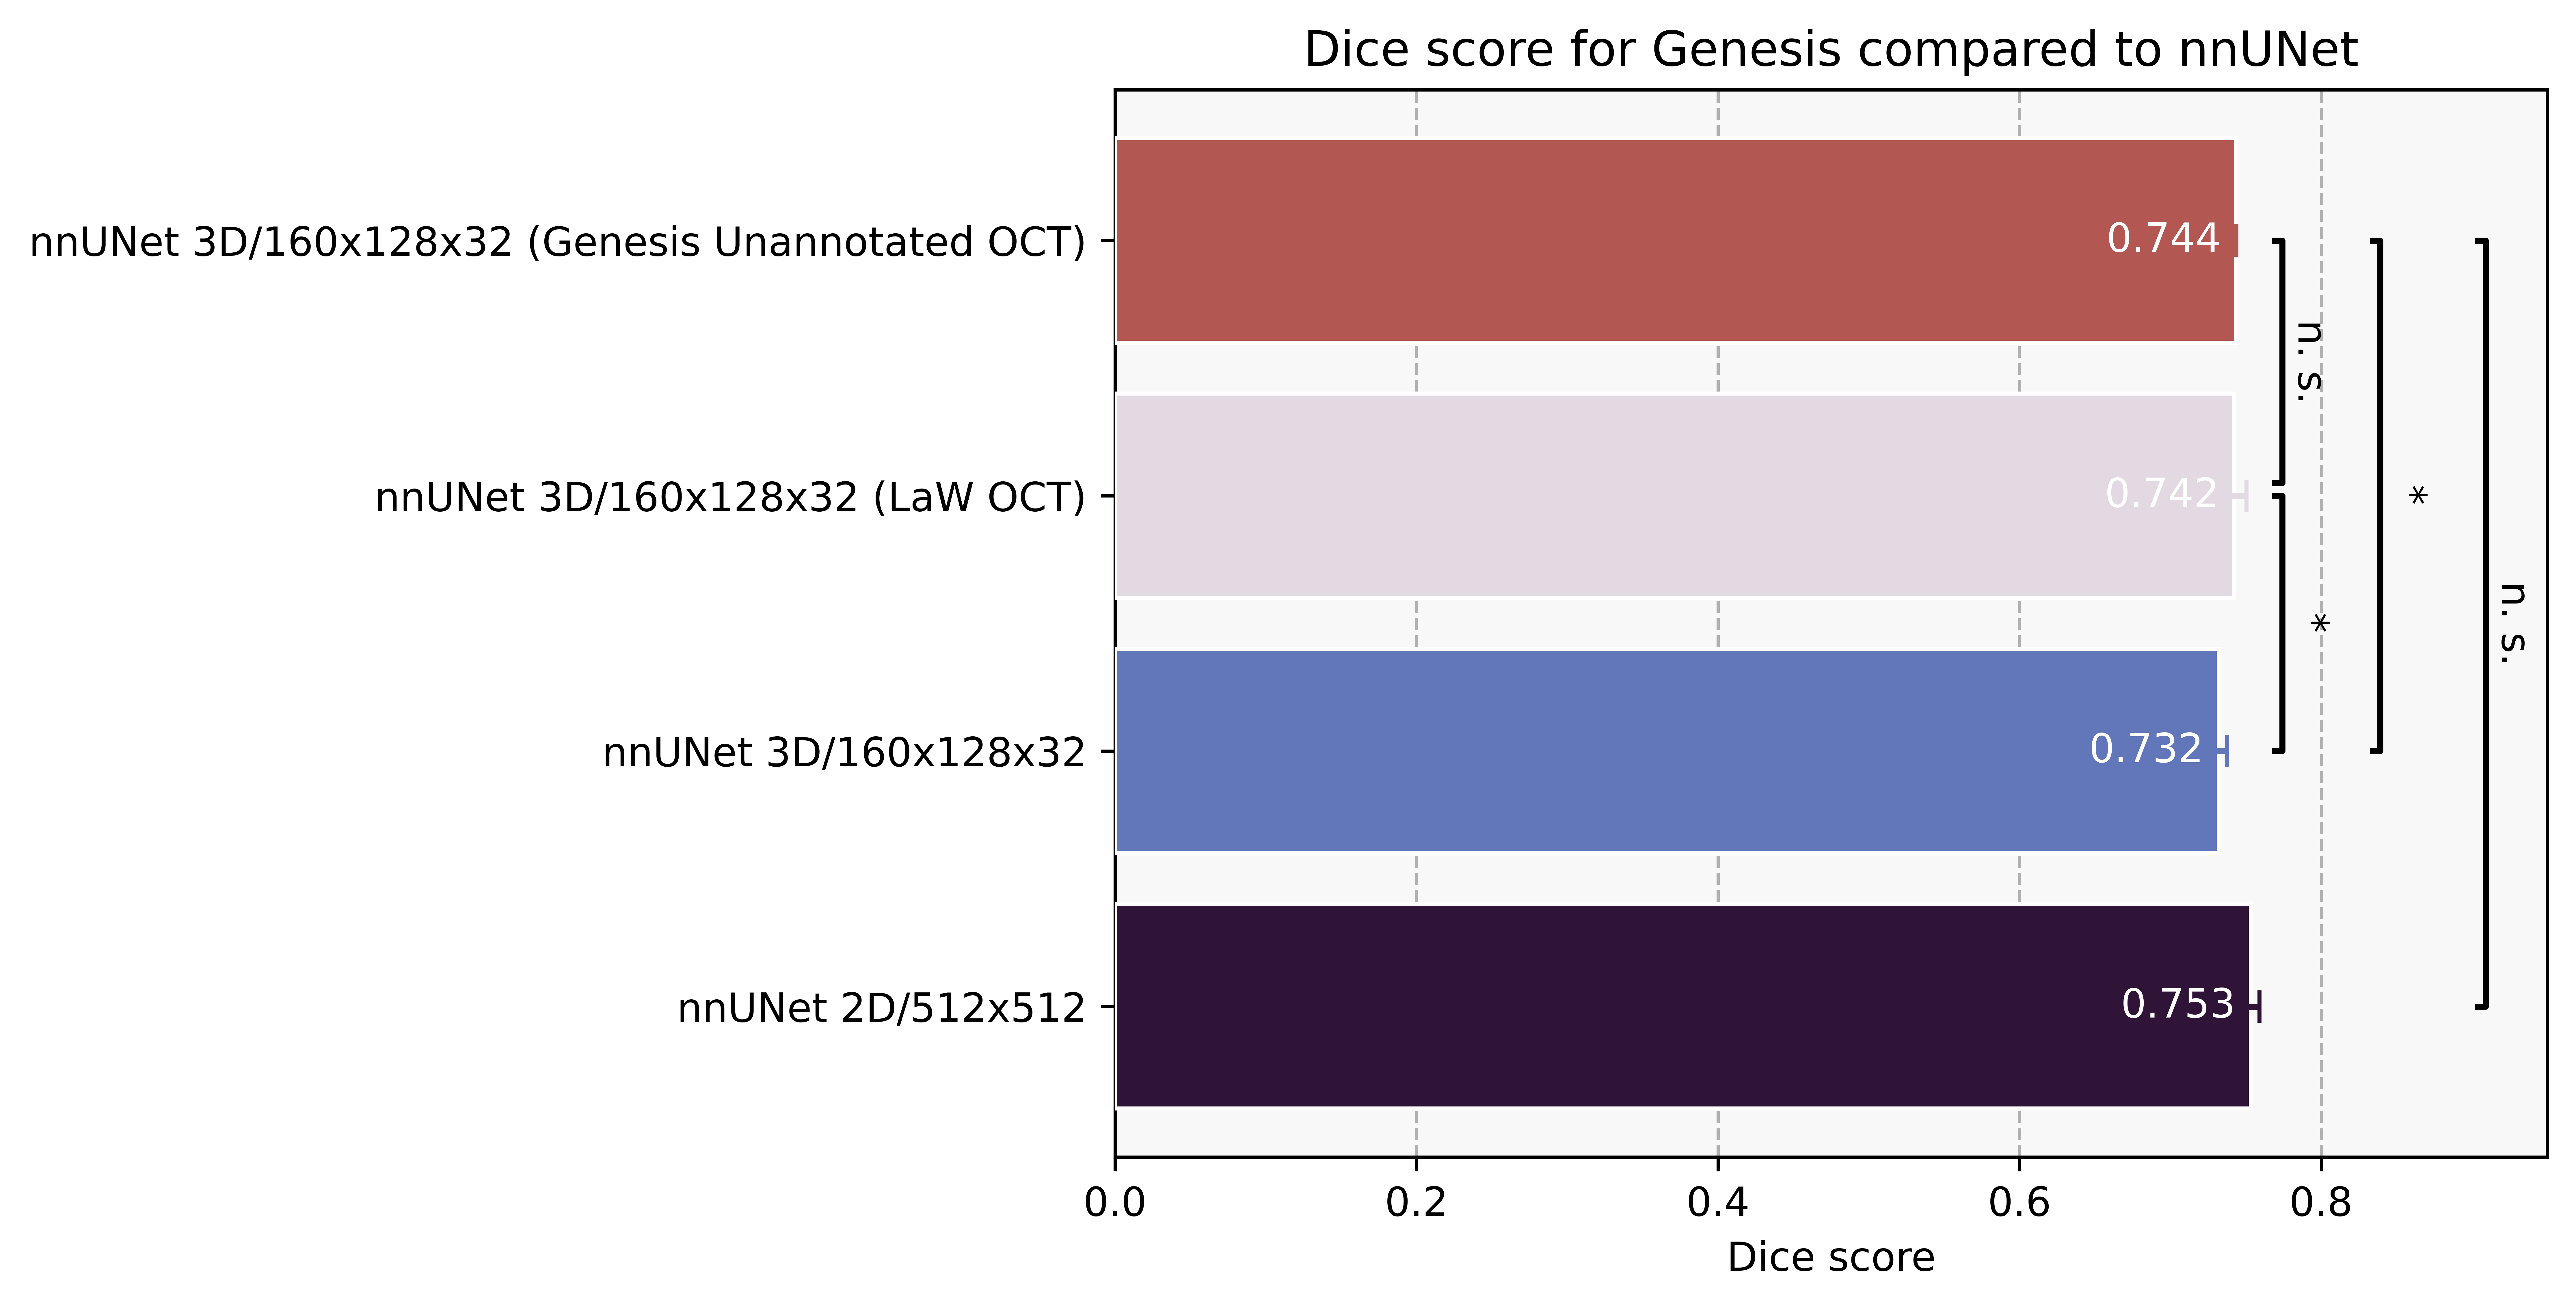
\includegraphics[width=0.65\linewidth]{figures/result_nnUNet_and_Genesis_results.png}
    \caption{Dice score of Genesis on the Calcium OCT dataset compared to that of nnUNets. The dataset used for pre-training is indicated in parentheses.
    }
    \label{fig:genesis-results}    
\end{figure}

Prior experience with nnUNet suggests that the lumen and wall are crucial features for improving calcium segmentation. We speculate that these features can also be learned by Genesis without needing annotations. By restoring corrupted images, the Genesis model might acquire a general understanding of the arterial anatomy, including the lumen and wall, which could aid in identifying calcified plaques. We support this hypothesis by visualizing the PCA of features from nnUNet pre-trained with Genesis, revealing that features around the arterial wall were clearly discernible (a pattern similar to CLIP; see Figure~\ref{fig:pca-genesis}). 

\begin{figure}[h]
    \centering
    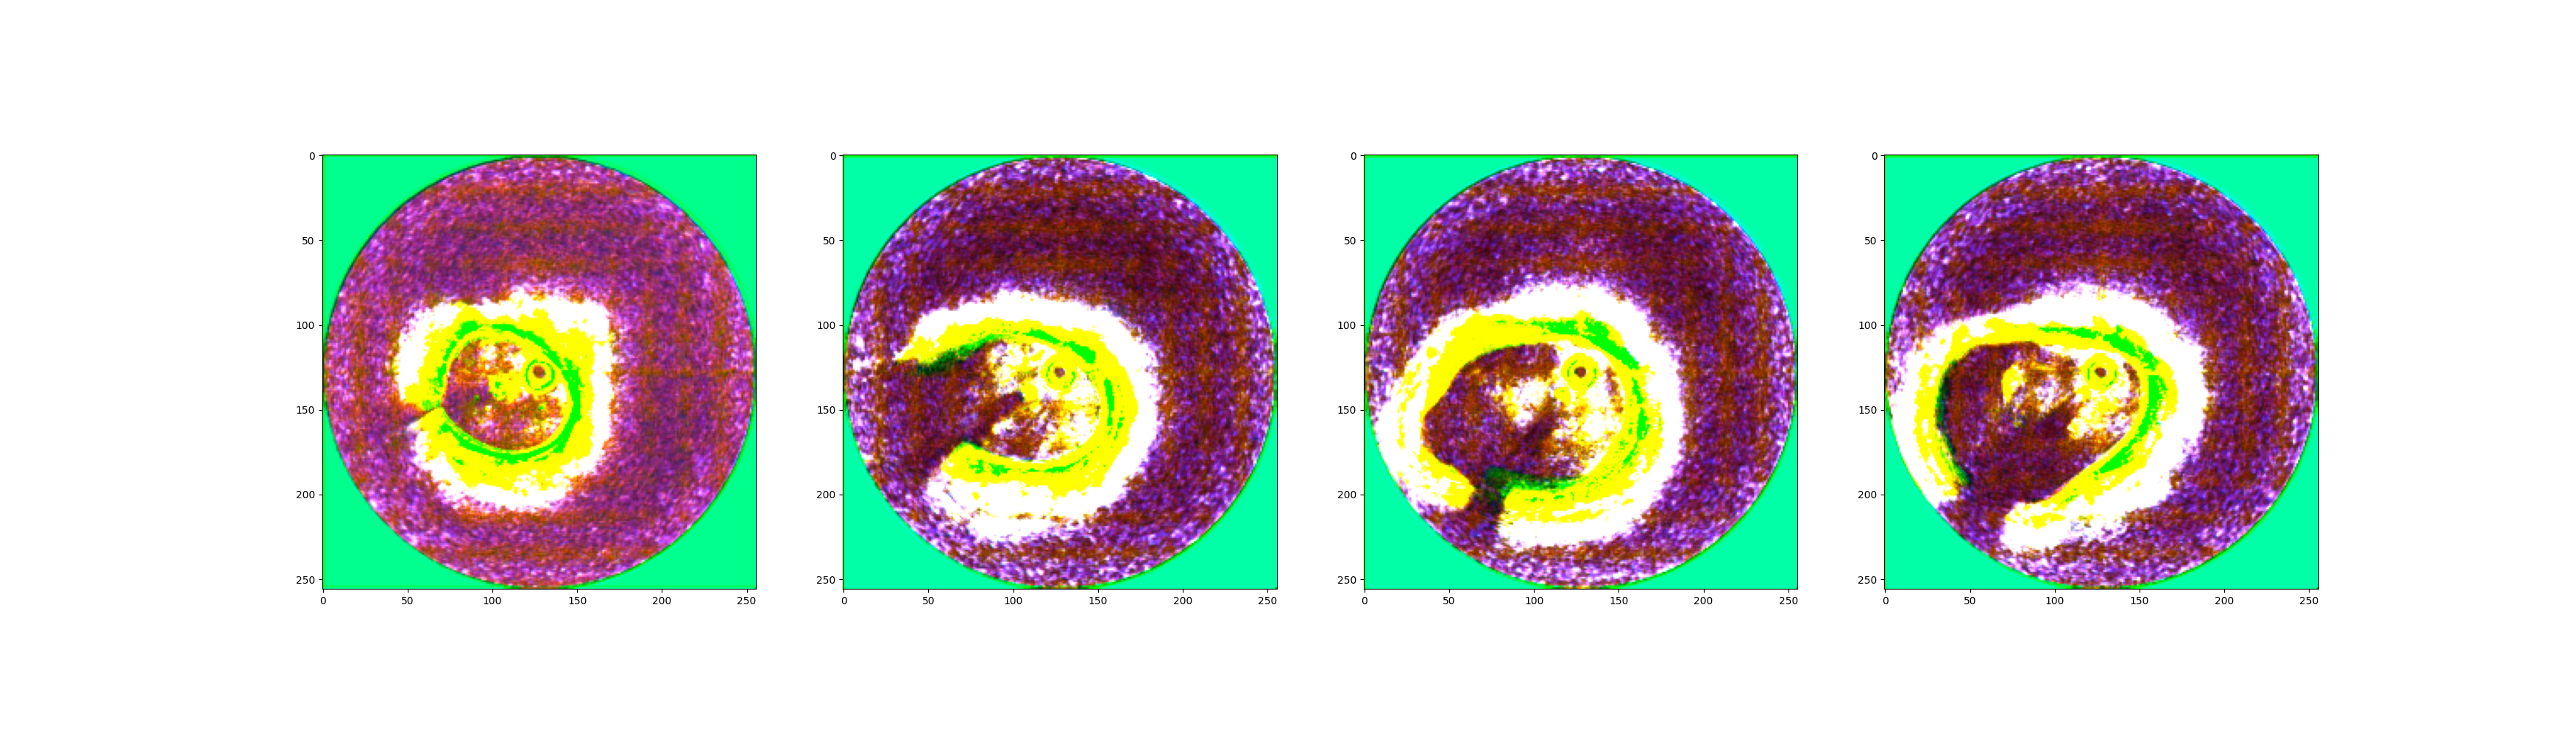
\includegraphics[width=0.5\linewidth]{figures/discussion_genesis_feature_map_batch0_feature1.png}
    \caption{PCA of the output of the features from the model pre-trained with Genesis}
    \label{fig:pca-genesis}
\end{figure}


\section{Final Results}
The models used in our study were categorized into two distinct groups: supervised learning and self-supervised learning (SSL). All results were statistically compared against the 2D nnUNet model, which demonstrated the highest average Dice score among the models evaluated and hence served as the highest standard for comparison. A summary of the best-performing models from each category is presented in Figure~\ref{fig:results}.

\begin{figure}[hbt]
    \centering
    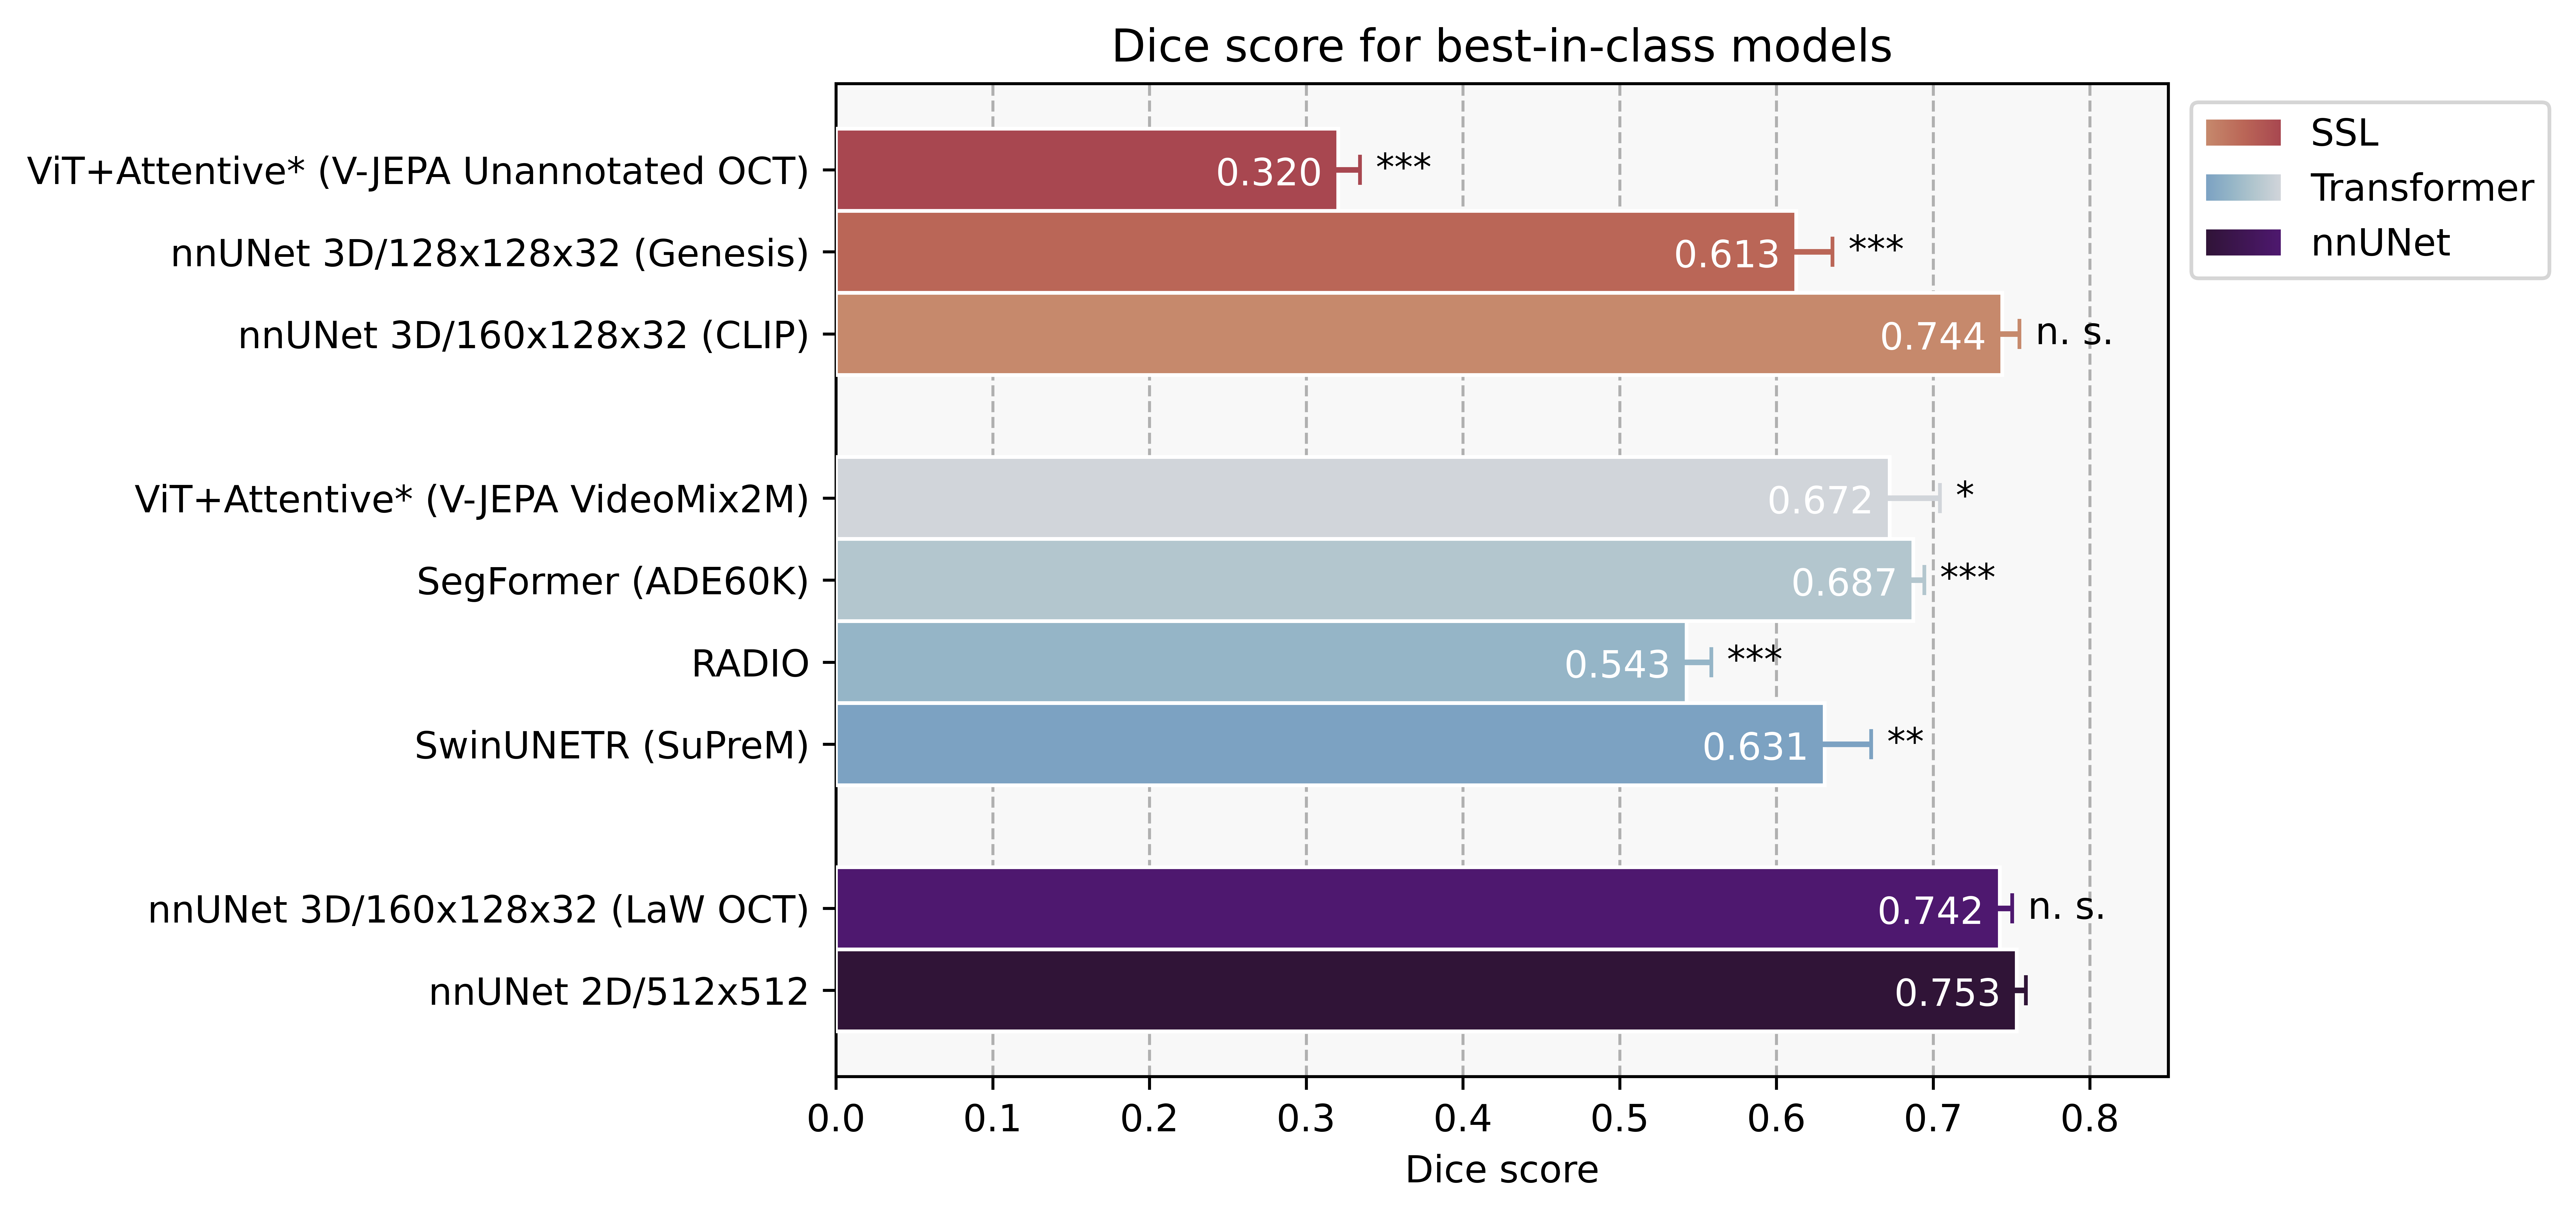
\includegraphics[width=1\textwidth]{figures/result_best_in_class_results.png}
    \caption{Summary of the results of the best models from each category. SSL denotes self-supervised learning models. Statistical significance indicates comparison against 2D nnUNet.}
    \label{fig:results}
\end{figure}

In the SSL category, V-JEPA pre-trained on unannotated OCT images performed significantly worse than 2D nnUNet. This discrepancy may be attributed to the dataset scale, which plays a crucial role in V-JEPA as discussed previously. By contrast, Genesis and CLIP pre-trained on unannotated OCT images achieved performance comparable to 2D nnUNet and were as effective as 3D nnUNet pre-trained on LaW OCT, despite needing minimal to no annotations. These results highlight the importance of pre-training and demonstrate that self-supervised pre-training using Genesis or CLIP is a viable and cost-effective alternative to supervised learning.

The Dice scores of SegFormer, RADIO, and SuPreM were significantly lower than that of 2D nnUNet. We hypothesize that this difference arose because nnUNet is specifically designed for small datasets, whereas transformer-based models typically assume access to moderately large datasets. As such, nnUNet appears to be more suitable for our limited dataset. Conversely, increasing the size of the dataset and model parameters may not provide further benefits for nnUNet beyond a certain point, whereas transformers are likely to benefit from scaling~\cite{Zhai2021}. This study does not intend to suggest that nnUNet is universally superior to transformers. Rather, it demonstrates that nnUNet is more appropriate for calcium segmentation in OCT images given the current scale of our dataset and model parameters.

2D nnUNet stood out as the top-performing model, achieving an average Dice score of $0.753 \pm 0.006$. Interestingly, this model did not benefit from additional pre-training on LaW OCT, likely because the dataset already provided sufficient training samples when converted into 2D images.

3D nnUNet performed best when the model was pre-trained on the LaW OCT dataset. Patch size played a critical role in the 3D nnUNet performance. Reducing the patch size in the width and height dimensions did not improve performance. We attribute this observation to the characteristics of calcified plaques in OCT images. Plaques are identified by intensity changes around artery walls, which are confined to a relatively small and narrow space within an OCT image. Expanding the width and height dimensions beyond these walls does not provide additional useful information for the model, resulting in no performance improvement. 

By contrast, reducing the patch size in the depth dimension significantly improved the model’s accuracy. Plaques frequently co-occur across adjacent slices, making additional context in the depth dimension less critical. Reducing the depth dimension not only was harmless to the model but also provided additional slices for training the model, which was highly beneficial given that the Calcium OCT dataset is small. The Dice score of 3D nnUNet pre-trained on Law OCT is smaller but not statistically significantly different from that of 2D nnUNet. 

Furthermore continuity is better achieved and retained during post-processing by 3D nnUNet, supporting its use in cases where continuity is required, such as for 3D digital twin reconstruction of the artery. %using a large patch size reduces the number of samples available for training the model, which is a critical consideration given that the Calcium OCT dataset is relatively small.

\section{Discussion}
\subsection{Scale Analysis}
The impact of dataset size on model performance was investigated by systematically subsampling the Calcium OCT dataset and evaluating the resulting models. We first set aside part of the Calcium OCT dataset to serve as a common test set for all models. We then randomly subsampled 33\%, 50\%, 66\%, and 83\% of the remaining Calcium OCT dataset and split each subset into 75\% and 25\% for training and validation, respectively. We trained models with the training set and tracked the best models with the validation set. The final Dice scores and cross entropy losses were calculated using the common test set. The analysis was performed for 3D nnUNet models trained from scratch, pre-trained on LawOCT, pre-trained with CLIP, or pre-trained with Genesis. Results are summarized in Figure~\ref{fig:scale-analysis}. 

We observed a positive correlation between Dice score and dataset scale regardless of the model used, consistent with conventional wisdom that model performance depends on the amount of data available for training. Given the small size of the Calcium OCT dataset, model performance was highly sensitive to the selection of training data, which led to significant volatility and a high standard deviation. This outcome is unsurprising, as small datasets typically contribute to greater variability in model performance.

\begin{figure}[hbt]
    \centering
    \begin{subfigure}[t]{0.49\textwidth}
        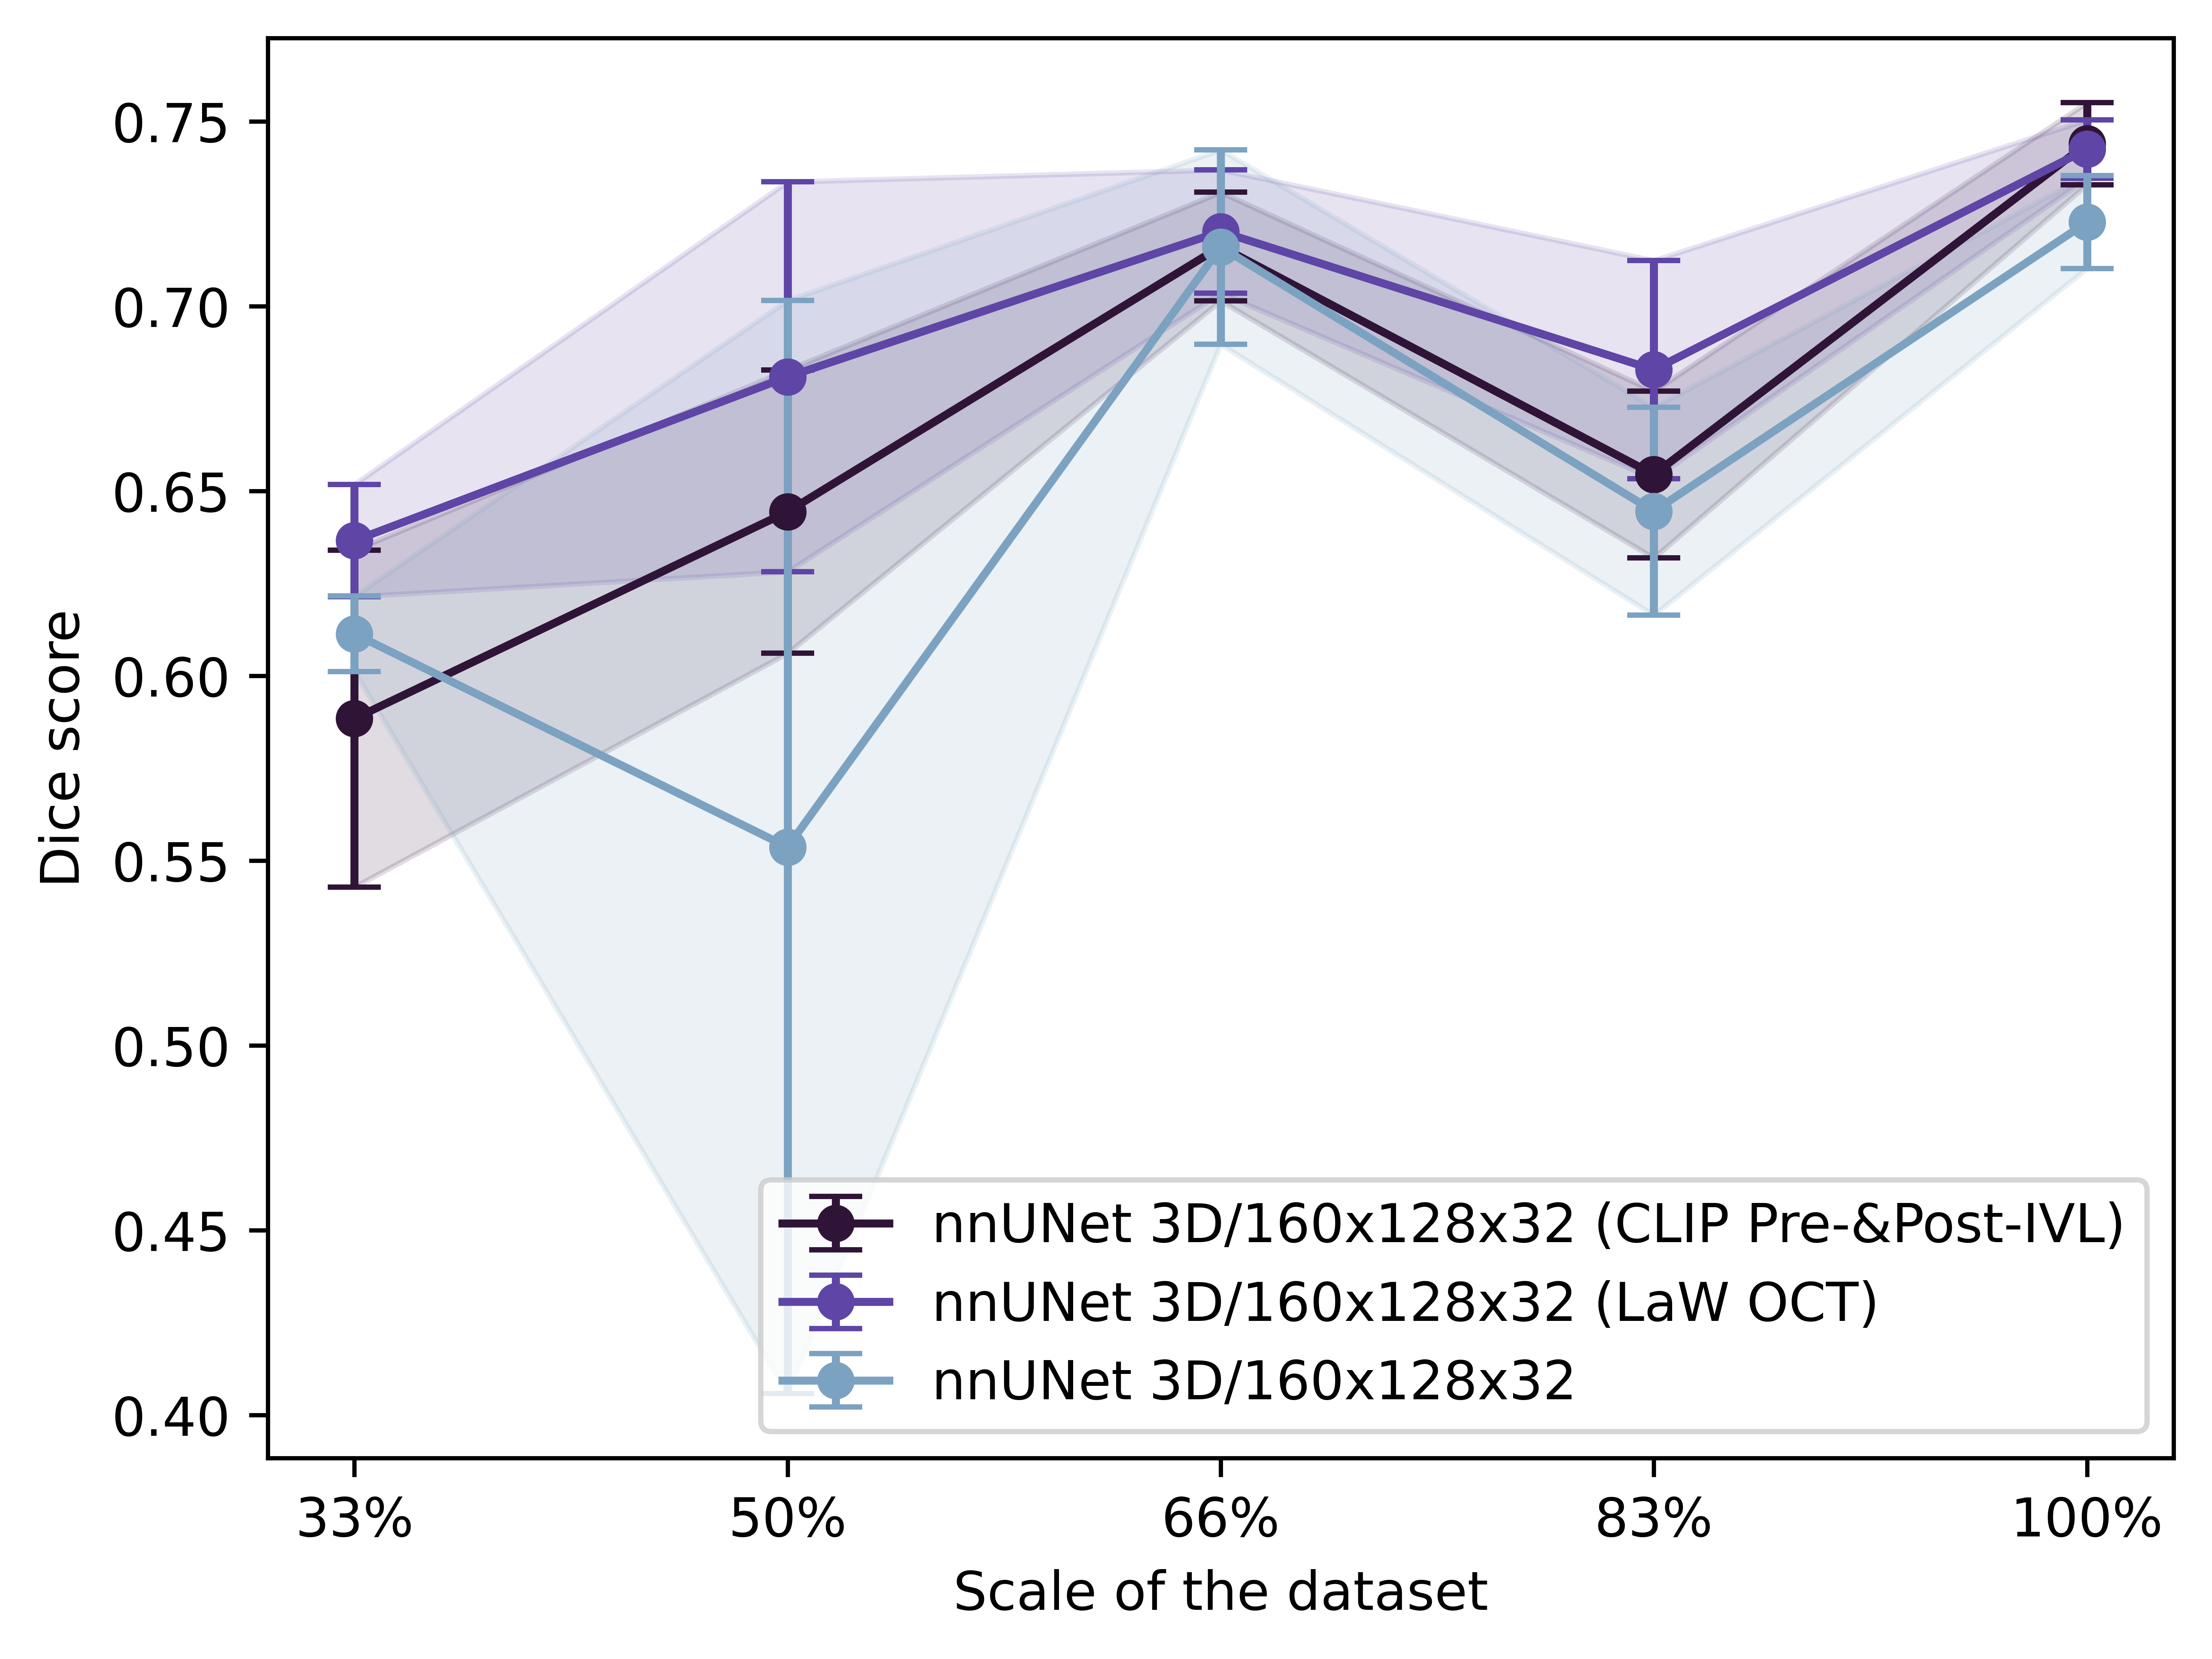
\includegraphics[width=1\linewidth]{figures/discussion_scale_analysis.png}
        \caption{Dice score scale analysis.}
        \label{fig:scale-analysis}
    \end{subfigure}%
    \begin{subfigure}[t]{0.49\textwidth}
        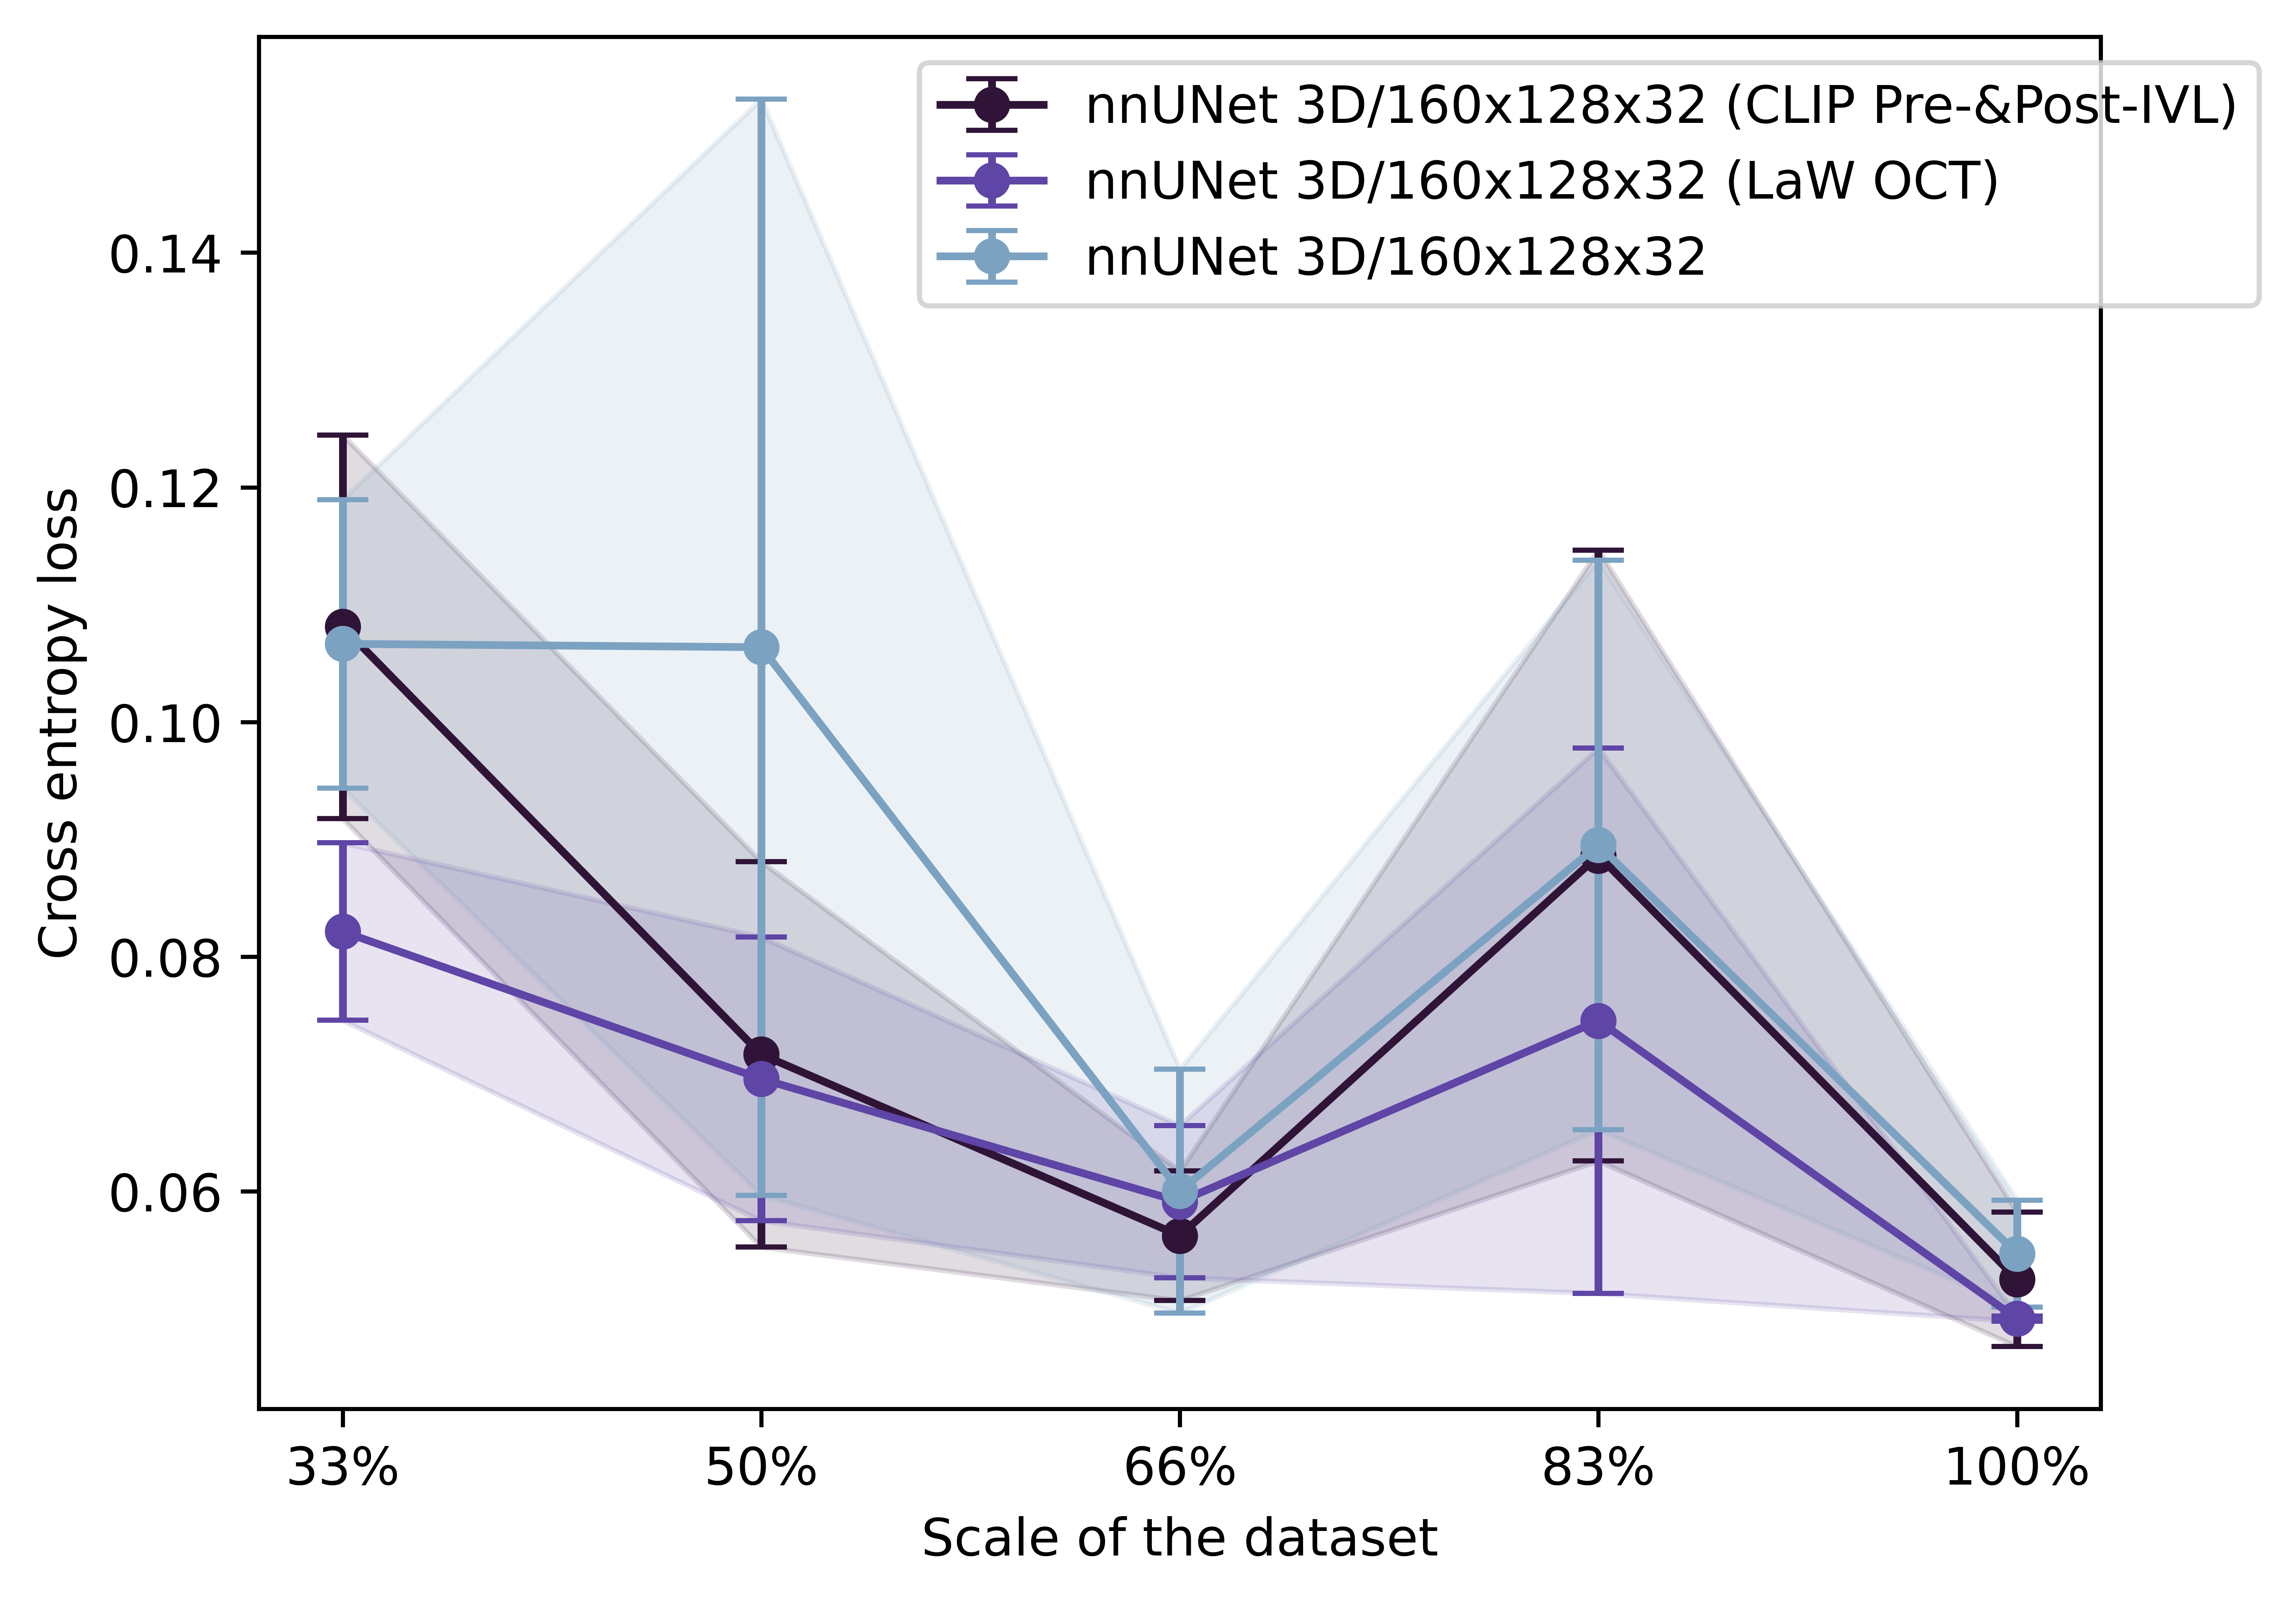
\includegraphics[width=1\linewidth]{figures/discussion_cross_entropy_scale_analysis.png}
        \caption{Cross entropy loss scale analysis.}
        \label{fig:cross-entropy-scale-analysis}
    \end{subfigure}
    \caption{Scale analysis of 3D nnUNets trained on the Calcium OCT dataset, subsampled at different scales. The values are shown in a moving average with a window size of 3.}
\end{figure}

Supervised pre-training on the LaW OCT dataset is more reliable than the other models, resulting in a higher averaged Dice score, as demonstrated in Figure~\ref{fig:scale-analysis}. Additionally, both self-supervised pre-training methods are more beneficial than training the model from scratch. These findings underscore the importance of leveraging pre-training, particularly on smaller datasets, to exchange model performance and stability.

Cross entropy loss provides a quantitative measure for the confidence and accuracy of a model's predictions. When the model is confident in a correct prediction, the loss is low, reflecting accurate performance. Conversely, if the model is confident in an incorrect prediction, the loss is high, reflecting poor performance. Model confidence and accuracy are important as they help users trust the automated segmentation process, ensuring that the results are reliable and can be confidently used in decision-making. The mathematical definition of binary cross-entropy loss is as follows.

\begin{equation}
-\frac{1}{N}\sum_{i=1}^{N}\left[y_{i}\cdot\log\left(p(y_{i})\right)+ \left( 1-y_{i} \right)\cdot \log\left(1 - p(y_{i})\right) \right]
\end{equation}

There was a negative correlation between cross entropy loss and dataset scale, consistent with conventional wisdom that more data results in higher model confidence and accuracy (Figure~\ref{fig:cross-entropy-scale-analysis}). Supervised pre-training on LaW OCT, CLIP, and Genesis all improved the cross entropy loss over 3D nnUNet, indicating that pre-training boosted model confidence and accuracy. 

CLIP and Genesis induced greater entropy losses than Law OCT-supervised pre-training. One possible explanation for this is that CLIP and Genesis "implicitly" learn the features related to the lumen and wall whereas Law OCT-supervised pre-training "explicitly" learns these features. Consequently, CLIP and Genesis may require a larger dataset to effectively translate implicit features into explicit ones during fine-tuning. In support of this hypothesis, Figure~\ref{fig:cross-entropy-scale-analysis} shows that CLIP and Genesis at 83\% data achieved a similar cross entropy loss as Law OCT at 50\%, suggesting that self-supervised methods may benefit from larger datasets to maximize performance. 

Even though self-supervised learning models (CLIP and Genesis) exhibited slightly poorer cross entropy losses than supervised pre-training, they also required fewer resources and could serve as viable alternatives for improving prediction in resource-constrained environments. Overall, the choice between supervised pre-training and self-supervised methods depends on the specific resource constraints and performance requirements of the application.

\subsection{Evaluating Features using PCA}
Visually appealing features do not always translate to better performance. Clarity of feature distinction often outweighs aesthetics. We compared features from V-JEPA (VideoMix2M) with those from the initial weights of the ViT model. As shown in Figure~\ref{fig:visually-good-features}, both sets of features preserved the structure of the artery walls. The V-JEPA (VideoMix2M) features enhanced the contrast of the artery walls by using a uniform color for the background, thereby improving distinguishability. In contrast, the features derived from the ViT model's initial weights exhibited less contrast, with the artery walls blending into the background through a color gradient, making them less distinguishable. This suggests that features that appear visually appealing to humans may not necessarily be the most effective for the model to learn from, and the increased contrast may explain why the V-JEPA (VideoMix2M) model performed better than ViT. 


\begin{figure}[hbt]
    \centering
    \begin{subfigure}[t]{0.8\textwidth}
        \centering
        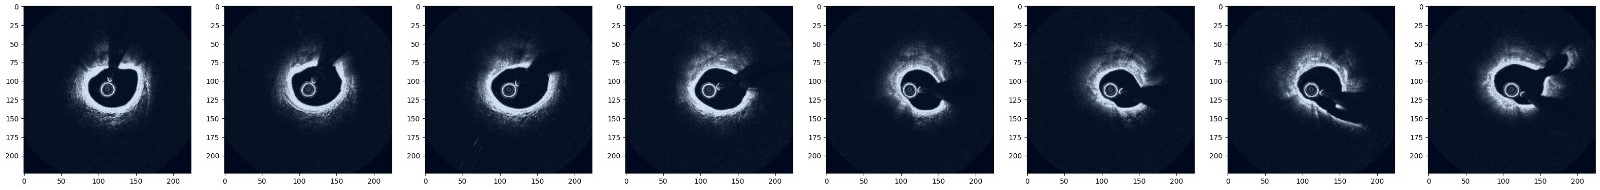
\includegraphics[width=0.9\linewidth]{figures/discussion_visual_vjepa_input.jpg}
        \caption{Input image}
    \end{subfigure}\\
    \begin{subfigure}[t]{0.8\textwidth}
        \centering
        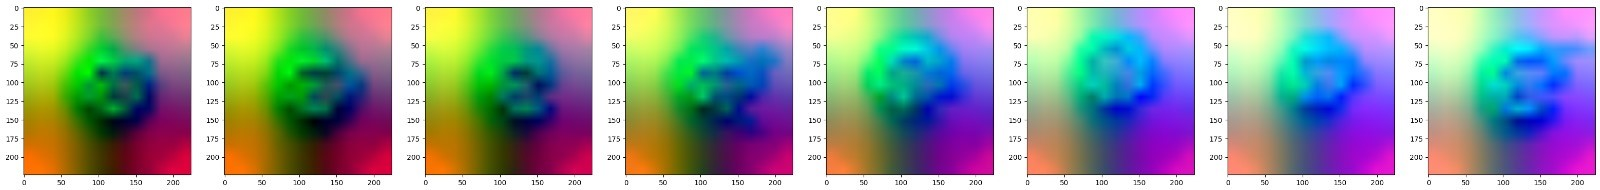
\includegraphics[width=0.9\linewidth]{figures/discussion_visual_vjepa_initial.jpg}
        \caption{PCA feature from ViT with initial weight}
    \end{subfigure}\\
    \begin{subfigure}[t]{0.8\textwidth}
        \centering
        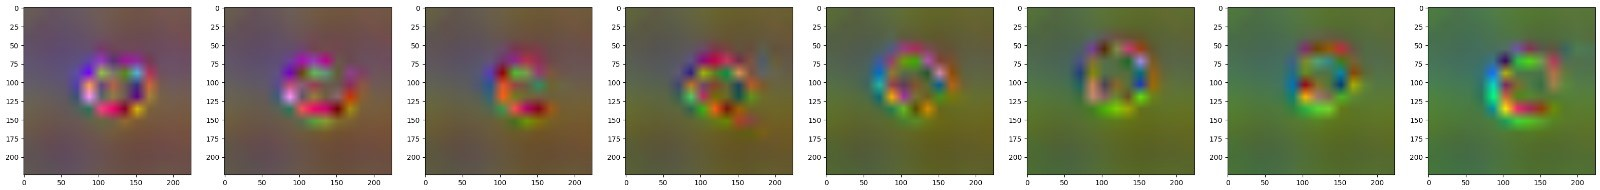
\includegraphics[width=0.9\linewidth]{figures/discussion_visual_vjepa_pretrained.jpg}
        \caption{PCA feature from ViT with V-JEPA pre-trained weight}
    \end{subfigure}
    \caption{PCA of the output features from the initial weight of the model and the features learned by V-JEPA. The volume is unrolled along the depth dimension.}
    \label{fig:visually-good-features}
\end{figure}

This hypothesis was further supported by visualization of features from ViT (RADIO). As shown in Figure~\ref{fig:radio-features}, these features are interpretable by humans and can effectively delineate OCT image semantics. The border between the background and the areas where the waves propagate is clearly visible, forming a distinct circle. However, the features representing the artery walls lack distinctiveness, which may account for the low Dice score of the ViT (RADIO) model.

\begin{figure}[hbt]
    \centering
    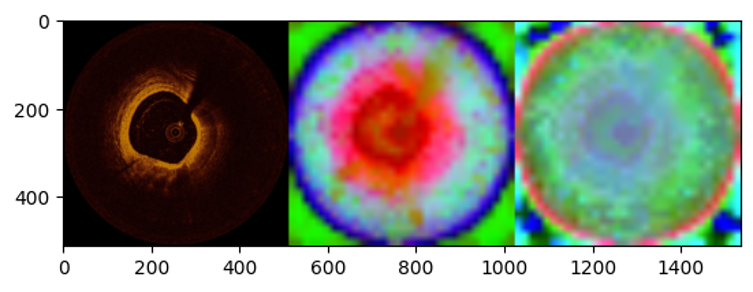
\includegraphics[width=0.35\textwidth]{figures/discussion_radio_feature.png}
    \caption{PCA of output features from ViT (RADIO). The middle column shows PCA with the first principal component retained, while the right column shows PCA with the first principal component removed.}
    \label{fig:radio-features}
\end{figure}

\subsection{V-JEPA Pre-training}
Unlike Genesis, where loss and semantic checks of the model's learning on the pre-text task can be easily determined, V-JEPA does not provide such clarity. We experimented with different configurations of V-JEPA pre-training on our unannotated OCT images and faced difficulties in converging the loss. As shown in Figure~\ref{fig:v-jepa-training}, the loss curve of ViT-L (V-JEPA Unannotated OCT) is converging, but it is sensitive to the configurations used.

\begin{figure}[hbt]
    \centering
    \begin{subfigure}[t]{0.3\textwidth}
        \centering
        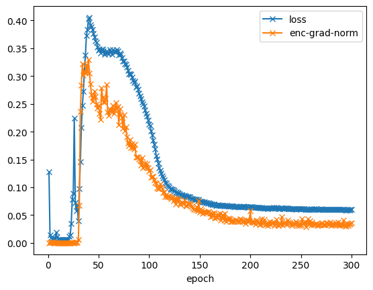
\includegraphics[width=0.9\linewidth]{figures/discussion_vjepa_training_1.png}
        \caption{ViT-L (V-JEPA Unannotated OCT)}
    \end{subfigure}\hfill%
    \begin{subfigure}[t]{0.3\textwidth}
        \centering
        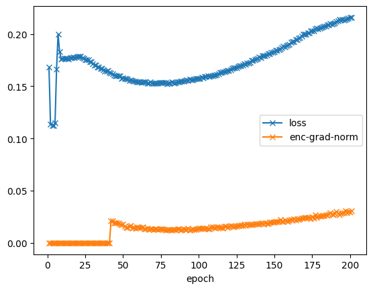
\includegraphics[width=0.9\linewidth]{figures/discussion_vjepa_training_2.png}
        \caption{ViT-S (V-JEPA Unannotated OCT)}
    \end{subfigure}\hfill%
    \begin{subfigure}[t]{0.3\textwidth}
        \centering
        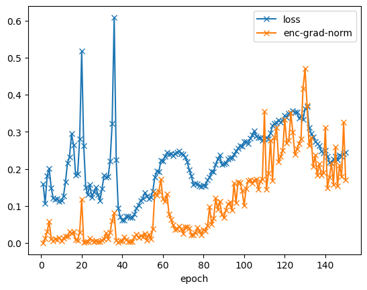
\includegraphics[width=0.9\linewidth]{figures/discussion_vjepa_training_3.png}
        \caption{ViT-L (V-JEPA Unannotated OCT) with more weight decay}
    \end{subfigure}
    \caption{Loss curves of V-JEPA pre-training on unannotated OCT images with various configurations.}
    \label{fig:v-jepa-training}
\end{figure}

One way to assess V-JEPA's convergence is by plotting and comparing the hidden features from the target encoder and the context encoder. The target encoder processes video patches without masking, while the context encoder does so with masking. As illustrated in Figure~\ref{fig:v-jepa-prediction}, successful pre-training in the V-JEPA framework enables accurate prediction of the hidden features for the masked-out parts of the video. Unlike Genesis or other pixel-level prediction tasks, it's challenging to determine whether the prediction is correct because the output is an embedding vector rather than a pixel-based prediction. This trade-off makes V-JEPA more computationally efficient than pixel-level tasks but also makes it harder to verify if the model is learning effectively.

\begin{figure}[hbt]
    \centering
    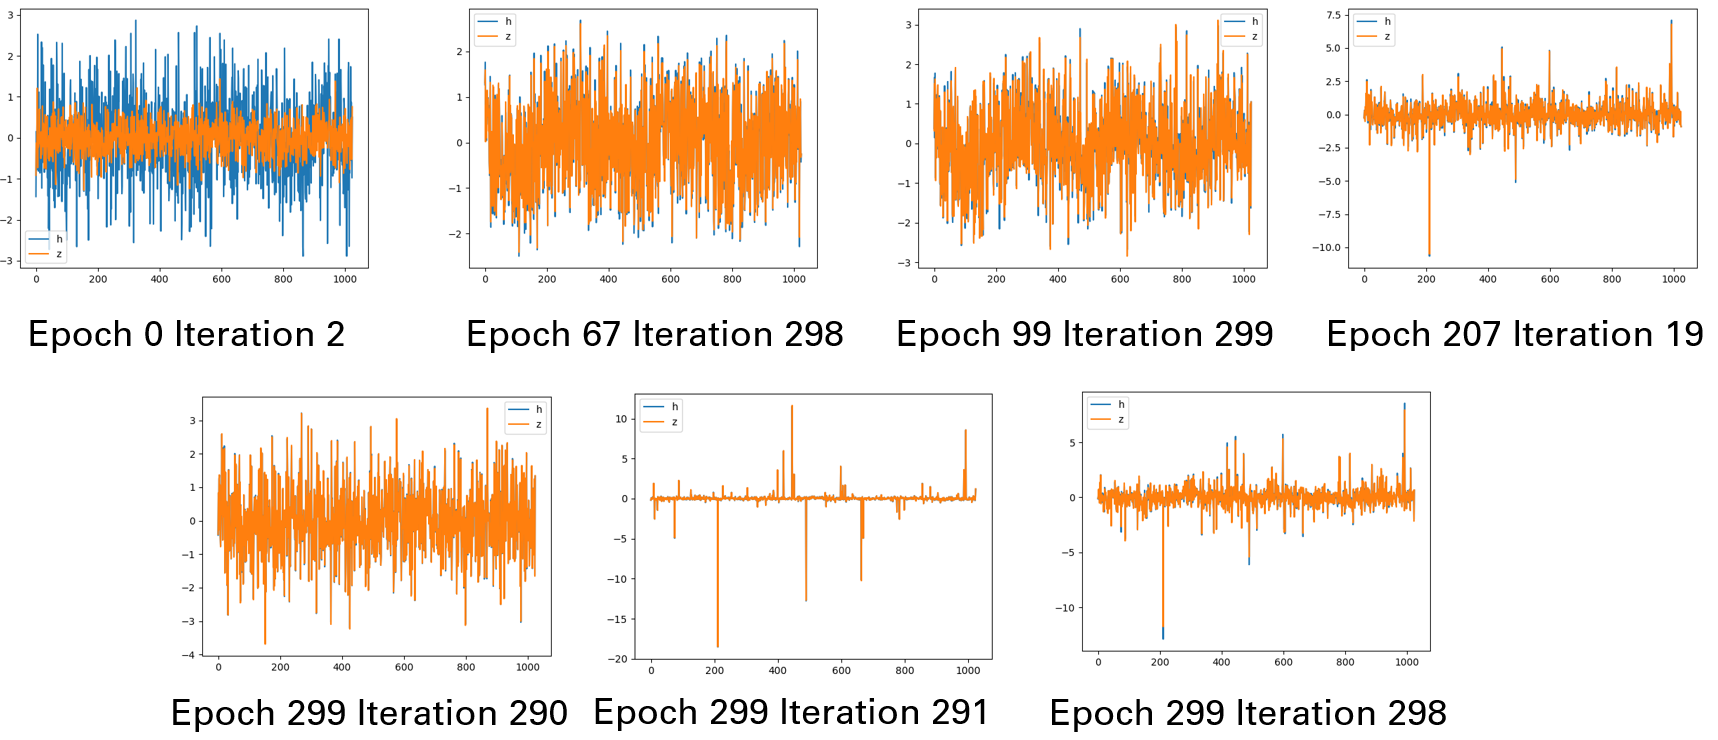
\includegraphics[width=0.8\textwidth]{figures/discussion_vjepa_prediction.png}
    \caption{Hidden features from the target encoder (denoted as \(h\) and colored in blue) and the context encoder of ViT (V-JEPA on unannotated OCT data) (denoted as \(z\) and colored in orange) over training epochs. The bottom row highlights the differences in hidden features between the target encoder and context encoder in the final epoch.}
    \label{fig:v-jepa-prediction}
\end{figure}

\subsection{CLIP Pre-training}\label{sec:results:discussion:clip}
As mentioned in Section~\ref{sec:implementation:clip}, CLIP requires a shared encoder and projector for successful pre-training convergence. In this section, we present the sanity checks performed and their results, offering insights for future efforts to adapt CLIP to multi-modal imaging.

We began by performing a sanity check of CLIP by training the model to match the identical images, as illustrated in Figure~\ref{fig:clip-sanity-check-same-image}. This is a much simpler task, and configurations that fail to match identical images would be unlikely to succeed in matching co-registered multi-modal OCT images. By identifying and eliminating unsuccessful configurations early, we avoided prolonged training. Next, we trained the model to match Pre-IVL and Post-IVL images, as shown in Figure~\ref{fig:clip-sanity-check-different-image}. This is the primary task of CLIP. Our findings indicate that only a shared encoder and projector can effectively converge the losses in this context.

\begin{figure}[hbt]
    \centering
    \begin{subfigure}[t]{0.3\textwidth}
        \centering
        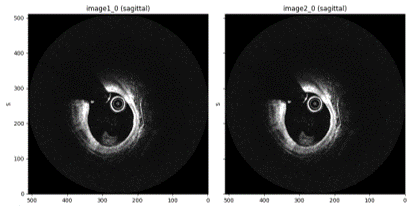
\includegraphics[width=0.9\linewidth]{figures/discussion_clip_same_image.png}
        \caption{Same images}
        \label{fig:clip-sanity-check-same-image}
    \end{subfigure}%
    \begin{subfigure}[t]{0.3\textwidth}
        \centering
        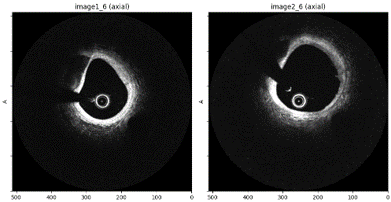
\includegraphics[width=0.9\linewidth]{figures/discussion_clip_pre-ivl_post-ivl_image.png}
        \caption{Pre-IVL and Post-IVL}
        \label{fig:clip-sanity-check-different-image}
    \end{subfigure}\\
    \begin{subfigure}[t]{0.3\textwidth}
        \centering
        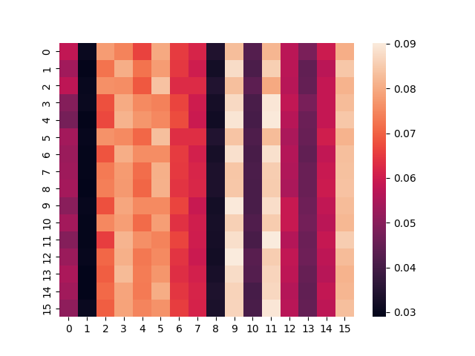
\includegraphics[width=0.9\linewidth]{figures/discussion_clip_same_image_diff_enc_diff_proj_logits.png}
        \caption{Co-similarity matrix of different encoders and projectors on the same images.}
        \label{fig:clip-cosimilarity-diff-enc-proj}
    \end{subfigure}%
    \hfill
    \begin{subfigure}[t]{0.3\textwidth}
        \centering
        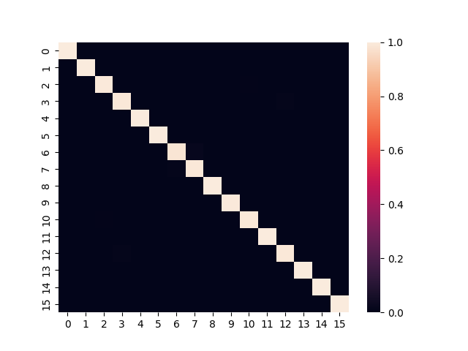
\includegraphics[width=0.9\linewidth]{figures/discussion_clip_same_image_diff_enc_shared_proj_logits.png}
        \caption{Co-similarity matrix of different encoders and shared projectors on the same images.}
        \label{fig:clip-cosimilarity-same-enc-proj}
    \end{subfigure}%
    \hfill
    \begin{subfigure}[t]{0.3\textwidth}
        \centering
        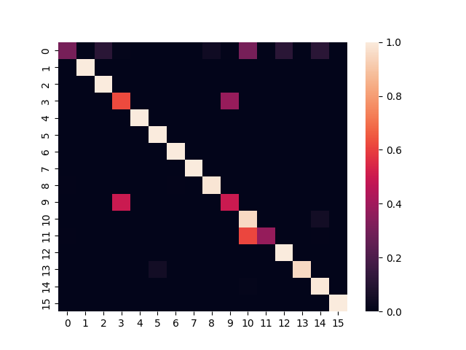
\includegraphics[width=0.9\linewidth]{figures/discussion_clip_same_image_shared_enc_shared_proj_logits.png}
        \caption{Co-similarity matrix of shared encoders and projectors on different modalities.}
        \label{fig:clip-cosimilarity-shared-enc-proj}
    \end{subfigure}
    \caption{Sanity check of CLIP. The model is trained to match the same images.}
    \label{fig:clip-sanity-check}
\end{figure}

To assess whether the model is learning effectively, we can plot a co-similarity matrix of the features output by the model. As shown in Figure~\ref{fig:clip-cosimilarity-diff-enc-proj}, when using different encoders and projectors, the loss did not converge, and the co-similarity matrix did not resemble an identity matrix. In contrast, with a shared projector, the loss converged using the same images, resulting in a co-similarity matrix closely resembling an identity matrix, as shown in Figure~\ref{fig:clip-cosimilarity-same-enc-proj}. However, the model did not converge when trained on different image modalities unless both the encoders and projectors were shared. Under these conditions, the co-similarity matrix appeared close to an identity matrix, as shown in Figure~\ref{fig:clip-cosimilarity-shared-enc-proj}.

Unlike language and image, different OCT image modalities are not as distinct from one another. Therefore, using different encoders and projectors to align hidden features may introduce noise during the initial training phase, preventing the model from converging.
%%%%%%%%%%%%%%%%%%%%%%
\chapter{Related Work}
%%%%%%%%%%%%%%%%%%%%%%

% The related work section covers closely related work. Here you can highlight
% the related work, how it solved the problem, and why it solved a different
% problem. Do not play down the importance of related work, all of these
% systems have been published and evaluated! Say what is different and how
% you overcome some of the weaknesses of related work by discussing the 
% trade-offs. Stay positive!

% This section is usually 3-5 pages.

% Self-supervised learning
\section{Self-supervised learning}
Self-supervised learning (SSL) has emerged as a promising approach for natural language processing (NLP). SSL is typically divided into two stages: pre-text tasks and downstream tasks. Pre-text tasks involve learning representations from the data itself without the need for human annotations. Once these representations are learned, downstream tasks use them to solve the primary objectives, which usually require human annotations. This approach enables models to learn robust representations while reducing the costs of human annotations~\cite{Jaiswal2020}. Although self-supervised pre-text tasks are widely used in the computer vision (CV) domain, identifying suitable pre-text tasks for visual SSL remains an active area of research. Examples of pre-text tasks in CV include autoencoder~\cite{Hinton2006}, denoising autoencoder~\cite{Vincent2008}, and colorization~\cite{Larsson2017}.

% Self-supervised learning in CVs
In recent years, both discriminative and generative tasks have been proposed as pre-text tasks in visual SSL. SimCLR, a discriminative method, learns representations by maximizing the similarity between differently augmented views of the same image while minimizing the similarity between views of different images~\cite{Chen2020Simple}. This approach, known as contrastive learning (CL), has shown to be effective for classification tasks, even outperforming supervised learning on ImageNet~\cite{Russakovsky2015} using the same ResNet50 architecture~\cite{He2016}. SimCLRv2 further improves SimCLR by incorporating a larger encoder, a projection head, and momentum contrast (MoCo)~\cite{He2020}, which uses a queue and a moving average encoder to stabilize training~\cite{Chen2020}. However, contrastive learning methods require a large batch size and a substantial number of negative samples to be effective~\cite{Chen2020Simple}. These requirements make it challenging to scale datasets and models.

On the contrary, generative learning generally predicts the data distribution to learn robust representations. Masked autoencoding (MAE) learns representations by generating pixel values of the masked-out parts of images, similar to the masked language modeling (MLM)~\cite{Devlin2019} in NLP~\cite{He2022}. MAE was initially explored using the vision transformer (ViT) model when the architecture was first proposed~\cite{Dosovitskiy2020vit}. However, its performance in the original study did not surpass that of supervised learning. To make this work, He et al. proposed masking out 75\% of an image rather than the previously experimented 50\%, and introduced asymmetric encoder-decoder architecture in MAE~\cite{He2022}. The encoder processes only the visible pixels, while the lightweight decoder operates on the encoded tokens. Compared to CL, MAE is less dependent on batch size, data augmentation, and the number of negative samples, rendering it more scalable. MAE outperforms supervised learning and supervised pre-training on ImageNet using the same ViT architecture and has been successfully evaluated on semantic segmentation such as ADE20k~\cite{Zhou2018}. Nonetheless, because MAE operates at a pixel level, it is computationally more expensive than CL.

While MAE focuses on reconstructing pixel values of masked patches, the bidirectional encoder for image transformer (BEiT) takes a different approach by first learning an image patch tokenizer and then predicting the tokenized values of the masked tokens, rather than the pixel values~\cite{Bao2022beit}. BEiT outperforms supervised learning and supervised pre-training on ImageNet~\cite{Russakovsky2015} and achieves state-of-the-art performance in semantic segmentation on ADE20k. However, the requirement for a tokenizer in BEiT adds complexity to the pre-text task compared to MAE. 

DINOv2 combines both restorative and discriminative pre-text tasks by learning representations by predicting the tokenized values of masked tokens and matching the class tokens of teacher and student networks, which encode different crops of the same image~\cite{Oquab2024dinov}. This approach has been shown to outperform other visual SSL methods of its time. Similar to BEiT~\cite{Bao2022beit}, DINOv2 is more efficient than pixel-level SSLs by performing representation learning at the token level. Building on this concept, I-JEPA takes it a step further, by directly predicting the encoded vectors of masked tokens instead of the tokenized values, removing the tokenizer from the approach. When evaluated on image classification, I-JEPA demonstrated comparable performance to other SSLs while being simpler and more efficient~\cite{Assran2023}. These advancements underscore the ongoing evolution and optimization of self-supervised learning techniques in visual representation learning.

Recent SSL methods have been extended to handle dynamic visual data, incorporating temporal dimensions to enhance visual SSL. VideoMAE, for instance, introduces tube masking to MAE~\cite{He2022} and employs an exceptionally high masking ratio of 90\%~\cite{Tong2022VideoMAE}. Without relying on external data, VideoMAE achieves state-of-the-art results on Kinetics-400~\cite{Kay2017Kinetics} and Something-Something V2~\cite{Goyal2017Something-SomethingV2} datasets. However, generating pixel values for video data imposes significant computational limitations, as video clips with numerous frames are challenging to process efficiently. V-JEPA, an extension of I-JEPA~\cite{Assran2023}, predicts the encoded vectors of masked patches in videos~\cite{Bardes2024Vjepa}. Given that I-JEPA is more efficient than MAE, V-JEPA offers a more efficient approach to learning representations in video data, outperforming VideoMAE in the process. These concepts can be applied to 3D medical images by substituting the temporal dimension with the depth axis.

% Self-supervised learning in medical imaging
\section{Self-supervised learning in medical imaging}
Self-supervised learning (SSL) offers significant benefits in medical imaging, where obtaining human annotations is both costly and time-consuming. Despite its potential, SSL methods have not been fully explored in the medical field, primarily due to the unique challenges it presents. One key challenge is the 3D nature of many medical images, unlike the 2D images typically used in SSL for natural images. Another challenge lies in the variety of medical imaging modalities, such as X-ray, CT, MRI, and ultrasound. In our study, we focus on optical coherence tomography (OCT) images of arteries, which are 3D and lack public datasets suitable for SSL. This presents a particular challenge, as no prior research has applied SSL to OCT images of arteries.

% Basic rotation, jigsaw, Rubik
Various classical visual SSL techniques have been explored to enhance segmentation tasks in medical imaging. For example, solving Rubik's cube has been used as a 3D pre-text task where the model learns to classify the orientation and order of a shuffled volumetric cube, leading to improved 3D brain tumor segmentation~\cite{Zhuang2019}. Similarly, the jigsaw-solving technique involves learning feature representations by predicting the correct order of shuffled image patches, leading to improved performance in tumor segmentation~\cite{Taleb2020}. Deep clustering groups feature vectors of the image in an unsupervised manner and use these clusters as pseudo-labels for classification~\cite{Caron2018}, leading to an improved abdominal organs classification~\cite{Dadoun2023}.

Applying one or multiple classical pre-text tasks has become a common theme in several SSL research within medical imaging~\cite{Zhou2021, Zhang2021, Dufumier2021}. For instance, Taleb et al. explored five distinct 3D self-supervised learning tasks, including predicting latent vectors of adjacent patches, predicting the location of a given patch, solving a jigsaw puzzle, predicting rotation angles, and contrastive learning ~\cite{Taleb2020}. Among these tasks, predicting latent vectors of adjacent patches resulted in the best performance in downstream tasks. Additionally, Song et al. combined rotation prediction, instance discrimination, and variation auto-encoder (VAE~\cite{Kingma2013}) as pre-text tasks~\cite{Song2022}. Using a VAE with an encoder-decoder equips the segmentation capability for COVID-19 infection segmentation on lung CT images. This approach outperformed supervised learning models with similar architectures, such as U-Net~\cite{Ronneberger2015} and U-Net++~\cite{Zhou2020}.

% Contrastive learning
Medical SSL research has increasingly focused on applying contrastive learning techniques to medical data.  TS-SSL is applied on 2D spectral domain optical coherence tomography (SD-OCT) images of the retina to improve retinal anomaly classification~\cite{Zhang2021}. TS-SSL simultaneously learns from classification, discriminative, and generative tasks. For the discriminative task, it employs contrastive loss to align different views of the same image. Concurrently, it predicts the rotation angle of rotated views and the order of the shuffled patches as generative tasks. Along with these pre-text tasks, TS-SSL classifies retinal anomalies of the SD-OCT images. However, this method only outperforms supervised learning when 10\% of the labeled data have been used for training. 

He et al.~\cite{He2022Intra} extended the application of contrastive learning to segmentation tasks by introducing intra- and inter-slice contrastive losses for point-supervised OCT fluid segmentation of the retina. Given that retinal OCT is three-dimensional, the authors utilized the correlation between adjacent slices within the same volume during the training of a U-Net~\cite{Ronneberger2015} segmentation model, using inter-slice contrastive loss. Segmented masks were subsequently used to identify small patches for intra-slice contrastive loss, which aimed to compare these patches with the background fluid patches. Simultaneously, the segmentation mask is also optimized by comparing the prediction with the ground truth using cross-entropy loss. This method outperformed other point-based segmentation techniques, although it did not achieve the same performance as fully supervised learning. Additionally, temporal consistency, akin to spatial consistency, can be leveraged to improve the segmentation of brain MRI images, especially when images are acquired from the same patient at different time points~\cite{Ren2022}.

Contrastive learning also facilitates the integration of different data modalities. Dufumier et al.~\cite{Dufumier2021} used patient age as a measure of similarity between different images, which improved the classification of bipolar disorder, Alzheimer's, and schizophrenia on 3D brain MRI images. Furthermore, the incorporation of tabular medical records into medical imaging can be done through Contrastive Language-Image Pre-training (CLIP)~\cite{Radford2021CLIP}, which aligns text with corresponding images. This approach has been shown to enhance classification tasks on brain MRI images~\cite{Hager2023}.

% Restorative tasks
Restorative tasks have emerged as effective pre-text tasks in medical imaging, particularly in settings where data is scarce. One such task is patch shuffling, which has been applied to 2D medical images from MRI, CT, and ultrasound. This task involves distorting an image by randomly cutting and pasting patches within it, and then challenging the model to restore the original image. This method has been shown to enhance downstream segmentation tasks in data-limited environments~\cite{Chen2019}.Similarly, in-painting, where a model predicts and fills in a missing part of an image~\cite{Pathak2016}, has demonstrated improvements in tissue segmentation for MRI and CT scans under data-scarce conditions~\cite{Dominic2023}.

Building on these ideas, the Genesis method combines several image distortion techniques to create 3D restorative pre-text tasks for CT images~\cite{Zhou2021}. Comprehensive experiments have shown that Genesis outperforms specialized 3D state-of-the-art segmentation models and other pre-text tasks, including denoising~\cite{Vincent2010}, in-painting~\cite{Pathak2016}, jigsaw~\cite{Noroozi2016}, deep clustering~\cite{Caron2018}, Rubik's cube solving~\cite{Zhuang2019}, and patch shuffling~\cite{Chen2019}. By integrating multiple restorative tasks, Genesis has set a new benchmark for 3D self-supervised learning (SSL) in medical imaging.  Following a similar approach, SwinUNTER~\cite{Tang2022} proposes training a transformer-based model using a combination of in-painting, contrastive learning, and rotation prediction to improve brain tumor segmentation in MRI images.

The success of Genesis has inspired follow-up research. TransVW extends Genesis by incorporating deep clustering~\cite{Caron2018} and adding a classification task to the restorative task framework of Genesis~\cite{Zhou2021}. In TransVW, visual words are automatically extracted and grouped into clusters using deep latent features. These visual words are then classified through deep clustering and restored using the Genesis method, resulting in improved segmentation and classification performance on some datasets compared to Genesis~\cite{Haghighi2021}. DiRA further enhances TransVW by introducing adversarial learning to distinguish between restored images and the original images~\cite{Haghighi2024}. Additionally, contrastive learning is employed as an additional pre-text task. By combining discriminative, restorative, and adversarial training, DiRA outperforms TransVW and models trained from scratch. However, despite these advancements, the evaluations of TransVW and DiRA are not as comprehensive as those for Genesis. TransVW only outperforms Genesis on certain datasets, while DiRA's performance is primarily evaluated against TransVW.

A gap exists between the pre-text tasks explored in medical imaging and those introduced in recent visual SSL research. While visual SSL research has shifted towards more efficient and simpler pre-text tasks such as DINOv2~\cite{Oquab2024dinov}, MAE~\cite{He2022}, and I-JEPA~\cite{Assran2023}, medical imaging SSL research has predominantly focused on blending multiple pre-text tasks. Genesis~\cite{Zhou2021} attempts to bridge this gap by establishing a modern restorative task as a new baseline for medical SSL. However, more studies are needed to evaluate the suitability of these modern visual SSL techniques in medical imaging. 

Recent studies have begun to explore this potential. Baharoon et al. applied DINOv2~\cite{Oquab2024dinov} directly to classification and segmentation tasks on X-ray, CT, and MRI images, demonstrating that self-supervised foundational models can effectively address medical imaging challenges~\cite{Baharoon2023general}. Similarly, Zhou et al. used MAE~\cite{He2022} pre-training on X-ray, CT, and MRI images and reported improvements in abdominal segmentation compared to UNETR baseline~\cite{Hatamizadeh2022}~\cite{Zhou2022}. These findings highlight the promising potential of modern visual SSL techniques in advancing medical imaging. Nevertheless, rigorous evaluation in medical imaging research must be done as many reported results may not be reproducible~\cite{Isensee2024}.

% Alternatives
\section{Self-supervised learning alternatives}
Self-supervised learning holds significant potential in medical imaging by enabling the extraction of useful representations from medical images without relying on human annotations. However, the development of effective pre-text tasks for SSL is still in its early stages, requiring extensive evaluation. Given the limited availability of large annotated medical datasets, it is crucial to explore alternative methods that can efficiently train models using small datasets.

One such alternative is supervised pre-training. The SuPreM approach, for example, advocates for pre-training models with supervised learning on large, annotated medical datasets. SuPreM compiles a dataset of 9,262 CT volumes annotated with abdominal organ segmentations. The models were initially pre-trained to segment a specific subset of these organs, and then fine-tuned to segment a different, non-overlapping set. The experiment demonstrated that supervised pre-training required less data to learn meaningful representations than self-supervised learning. Additionally, the representations learned through SuPreM exhibited strong transferability to different tasks and datasets.

Instead of pre-training, the nnUNet framework offers a self-configuring approach to medical image segmentation. This framework automatically builds a U-Net model for 2D and 3D medical images tailored to a given dataset. It has outperformed several state-of-the-art models, including popular transformer-based and Mamba-based architectures, on various medical image segmentation tasks. Notably, nnUNet is particularly effective on small datasets due to its robust data sampling and augmentation~\cite{Isensee2020}. Subsequent study on nnUNet underscores that it consistently demonstrates superior performance on the evaluated tasks without the need for additional data~\cite{Isensee2024}.

Another prevalent approach involves fine-tuning models that were pre-trained on different datasets. For instance, SegFormer, a state-of-the-art model for semantic segmentation, was initially trained on the ADE20k dataset. This model leverages a transformer-based architecture that hierarchically processes input features through multiple transformer blocks, capturing both local and global context effectively. SegFormer uses simple multilayer perceptron (MLP) decoder heads that aggregate features from different depths, combining information across scales to produce accurate segmentation masks~\cite{Xie2021SegFormer}. It has achieved state-of-the-art on semantic segmentation at the time, and has shown promising results when applied to other segmentation tasks~\cite{Ghosh2024, Khaled2023}.

Taking a different approach, RADIO proposes to learn representations from multiple teacher models. RADIO is a distillation framework with a student model tasked to predict the same feature as its teacher models, including DINOv2~\cite{Oquab2024dinov}, SAM~\cite{Kirillov2023SAM} and CLIP~\cite{Radford2021CLIP}. Furthermore, RADIO is resolution-agnostic, allowing it to interpret images at different resolutions. RADIO model has demonstrated the ability to generate high-resolution feature maps that can be utilized for several downstream tasks~\cite{Ranzinger2024RADIO}.

While self-supervised learning holds great potential in medical imaging, it is essential to compare SSL methods with existing alternatives to ensure a comprehensive understanding to their relative strengths and weaknesses.

%%%%%%%%%%%%%%%%%%%%
\chapter{Conclusion}
%%%%%%%%%%%%%%%%%%%%

% In the conclusion, you repeat the main result and finalize the discussion of
% your project. Mention the core results and why as well as how your system
% advances the status quo.
Self-supervised learning is a promising approach for medical imaging, as demonstrated through our work on calcium segmentation. Supervised learning has traditionally been the dominant method in this field due to its strong performance, but it has the significant drawback of requiring annotated data, which is both time-consuming and costly to obtain. Self-supervised learning, on the other hand, offers a cost-effective alternative by utilizing unannotated data while still achieving comparable performance, as we have shown in this study.

The choice of algorithm should depend on the availability of data. When relevant annotations are available, supervised learning remains the preferred method for calcium segmentation. However, when only co-registered data is accessible, the CLIP algorithm provides a viable alternative, offering better confidence and accuracy (as indicated by lower cross-entropy loss) compared to the Genesis model. In cases where annotations are unavailable, Genesis still presents a valuable option for enhancing calcium segmentation without the need for costly human annotations.

Looking ahead, future advancements in visual self-supervised learning could potentially eliminate the need for human annotation in medical imaging altogether, which would be a significant boon for both the medical community and patients.

% We ... evaluation of calcium segmentation based on its use cases. 
% For better segmentation accuracy, we identified that supervised pre-training on lumen and wall OCT images is the best approach i
% have 4 best algo , supervised 2d
% (1) Based on scaled analysis, supervised > self-supervised across scales of training data
% (2) SSL is comparable to supervised while being inexpensive
% (3) lumen and wall are keys features for improving calcium segmentation
% (4) 3D segmentation provides better continuous segmentation mask which is useful for training diffusion model for synthetic data


% \begin{enumerate}
%     \item Compared supervised and self-supervised learning techniques for calcium segmentation. 
%     \item Assessed the efficacy of pre-trained models from both self-supervised and supervised pre-training for calcium segmentation. 
%     \item Analyzed 2D and 3D segmentation approaches in the context of 3D digital twin reconstruction, focusing on the continuity of the masks produced by each method.
%     \item Evaluated self-supervised learning methods for medical imaging, including contrastive, restorative, and mask-image-modeling approaches, to bridge the gap between natural and medical visual self-supervised learning.
%     \item Proposed and evaluated segmentation heads for V-JEPA, a transformer-based self-supervised learning method for natural videos, and developed an approach to track its convergence during pre-training.
%     \item Suggested modifications to CLIP pre-training for multi-modal co-registered OCT images.
%     \item Proposed modifications to Genesis pre-training for unannotated OCT images. 
%     \item Analyzed the best methods across different scales of training data to provide insights into the suitability of each technique.
% \end{enumerate}


\cleardoublepage
\phantomsection
\addcontentsline{toc}{chapter}{Bibliography}
\printbibliography

% Appendices are optional
% \appendix
% %%%%%%%%%%%%%%%%%%%%%%%%%%%%%%%%%%%%%%
% \chapter{How to make a transmogrifier}
% %%%%%%%%%%%%%%%%%%%%%%%%%%%%%%%%%%%%%%
%
% In case you ever need an (optional) appendix.
%
% You need the following items:
% \begin{itemize}
% \item A box
% \item Crayons
% \item A self-aware 5-year old
% \end{itemize}

\end{document}